\documentclass[11pt,a4paper,oldfontcommands]{memoir}
\usepackage[utf8]{inputenc}
\usepackage[T1]{fontenc}
\usepackage{microtype}
\usepackage[dvips]{graphicx}
\usepackage{xcolor}
\usepackage{todonotes}
\usepackage{times}
\usepackage{amsmath}
\usepackage{natbib}
\usepackage{array}
\usepackage{listings}
\usepackage{pgf-umlsd}
\usepackage{parskip}

\setlength{\parskip}{10pt} %add space between paragraphs

%%% Fix the issue with \mess redefinition when importing msc
\let\msg\mess
\let\mess\undefined

\newcommand\draft{1}

\if1\draft
    \overfullrule=2cm
\fi

\lstset{
  language = C,
  basicstyle=\small,    % the size of the fonts that are used for the code
  stepnumber=1,                           % the step between two line-numbers. If it is 1 each line will be numbered
  numbersep=10pt,                         % how far the line-numbers are from the code
  tabsize=2,                              % tab size in blank spaces
  extendedchars=true,                     %
  breaklines=true,                        % sets automatic line breaking
  captionpos=b,                           % sets the caption-position to top
  mathescape=true,
  stringstyle=\color{white}\ttfamily,
  showspaces=false,           
  showtabs=false,             
  xleftmargin=17pt,
  framexleftmargin=17pt,
  framexrightmargin=17pt,
  framexbottommargin=5pt,
  framextopmargin=5pt,
  showstringspaces=false     
 }

\renewcommand\lstlistlistingname{List of Listings}
\newlistof{lstlistoflistings}{lol}{\lstlistlistingname}
\newcommand\typestyle{\rmfamily\mdseries\upshape}
\newcommand\addtypes[1]{%
  \lstset{morekeywords=[3]{#1}}}

\usepackage[
breaklinks=true,colorlinks=true,
%linkcolor=blue,urlcolor=blue,citecolor=blue,% PDF VIEW
linkcolor=black,urlcolor=black,citecolor=black,% PRINT
bookmarks=true,bookmarksopenlevel=2]{hyperref}

\usepackage{breakurl}

\usepackage{geometry}
% PDF VIEW
% \geometry{total={210mm,297mm},
% left=25mm,right=25mm,%
% bindingoffset=0mm, top=25mm,bottom=25mm}
% PRINT
\geometry{total={210mm,297mm},
left=20mm,right=20mm,
bindingoffset=10mm, top=25mm,bottom=25mm}

\usepackage{bytefield}
\usepackage{msc}

\OnehalfSpacing
%\linespread{1.3}

%%% CHAPTER'S STYLE
\chapterstyle{bianchi}
%\chapterstyle{ger}
%\chapterstyle{madsen}
%\chapterstyle{ell}
%%% STYLE OF SECTIONS, SUBSECTIONS, AND SUBSUBSECTIONS
\setsecheadstyle{\Large\bfseries\sffamily\raggedright}
\setsubsecheadstyle{\large\bfseries\sffamily\raggedright}
\setsubsubsecheadstyle{\bfseries\sffamily\raggedright}


%%% STYLE OF PAGES NUMBERING
%\pagestyle{companion}\nouppercaseheads 
%\pagestyle{headings}
%\pagestyle{Ruled}
\pagestyle{plain}\nouppercaseheads
\makepagestyle{plain}
\if0\draft
\makeevenfoot{plain}{\thepage}{Multipath DTLS: Design and Implementation}{}
\makeoddfoot{plain}{}{Q. Devos \& L. Fortemps de Loneux}{\thepage}
\makeevenhead{plain}{\leftmark}{}{}
\makeoddhead{plain}{}{}{\rightmark}
\else
\makeevenfoot{plain}{\thepage}{}{}
\makeoddfoot{plain}{}{}{\thepage}
\makeevenhead{plain}{}{}{}
\makeoddhead{plain}{}{}{}
\fi

\maxsecnumdepth{subsection} % chapters, sections, and subsections are numbered
\maxtocdepth{subsection} % chapters, sections, and subsections are in the Table of Contents


%%%---%%%---%%%---%%%---%%%---%%%---%%%---%%%---%%%---%%%---%%%---%%%---%%%

\begin{document}
%%%---%%%---%%%---%%%---%%%---%%%---%%%---%%%---%%%---%%%---%%%---%%%---%%%
%   TITLEPAGE
%
%   due to variety of titlepage schemes it is probably better to make titlepage manually
%
%%%---%%%---%%%---%%%---%%%---%%%---%%%---%%%---%%%---%%%---%%%---%%%---%%%
\if0\draft
\thispagestyle{empty}

{%%%
\sffamily
\centering
\Large

~\vspace{\fill}

EPL-2014 384\\
{\huge 
Multipath DTLS: Design and Implementation
}

\vspace{2.5cm}

{\LARGE
Quentin Devos \\
Loïc Fortemps de Loneux
}

\vspace{3.5cm}

A thesis submitted in partial fulfillment for the\\
Master in Computer Science Engineering\\[1em]
in the\\[1em]
Louvain School of Engineering\\
Université Catholique de Louvain

\vspace{3.5cm}

Supervisors: \\
Prof. Olivier Bonaventure\\
Prof. Olivier Pereira

\vspace{\fill}

June 2015

%%%
}%%%

\cleardoublepage
%%%---%%%---%%%---%%%---%%%---%%%---%%%---%%%---%%%---%%%---%%%---%%%---%%%
%%%---%%%---%%%---%%%---%%%---%%%---%%%---%%%---%%%---%%%---%%%---%%%---%%%

\tableofcontents*
\clearpage

\listoffigures*
\clearpage

\lstlistoflistings*
\clearpage

%%%---%%%---%%%---%%%---%%%---%%%---%%%---%%%---%%%---%%%---%%%---%%%---%%%
%%%---%%%---%%%---%%%---%%%---%%%---%%%---%%%---%%%---%%%---%%%---%%%---%%%

\chapter*{Introduction}
\markboth{Introduction}{}
\addcontentsline{toc}{chapter}{Introduction}

The Datagram Transport Layer Security (DTLS) provides security on top of datagrams protocols such as UDP. It was originally presented as an adaptation of TLS \cite{rfc5246} for unreliable communications by Modadugu \& Rescorla in 2004 \cite{modadugu2004design}. This new standard arised whereas some software developers already had built their own way of dealing with secure communications over UDP. However, the interest for this protocol is increasing and its integration in existing systems when security is needed is more and more considered \cite{dtls-as-subtransport}.

The main advantage of this protocol is its tolerance to frequent losses, which could be a requirement in some environment. This may also be helpful for real-time communication such as live streaming, where retransmission is not required. We will present later on all the potential applications that could benefit from using DTLS. Moreover, some existing commercial applications are already actively using it, like Cisco AnyConnect VPN\cite{anyconnect}.


Our objective in this master thesis is to assess the possibility to bring multipath ability to this protocol. Namely, we want to make it use multiple interfaces concurrently for the same DTLS session. This aspect have already been studied for other protocols such as MPTCP \cite{RFC6824} or MPRTP \cite{singh-avtcore-mprtp}. Nevertheless,we must keep in mind the additional security requirement and guarantee at least the same level of security as standard DTLS.

In the first chapter of this master thesis, we present additional details about DTLS with a short summary of the foundations inherited from TLS. We give an example of how a typical handshake will take place and how security is guaranteed. Then, we present an overview of application data exchange and how losses are handled. Finally, we review the security considerations of DTLS.

Chapter \ref{chap:mprtp} is giving an insight into an existing multipath protocol, MPRTP. This is probably the closest protocol we have to be inspired of. Indeed, it is most of time used with UDP and has also to deal with losses and reordering. This chapter concludes the first part dedicated to the state of the art.

The following chapters constitute the second part of this thesis and focus on our proposition : MPDTLS. Chapter \ref{chap:design} details the different design aspects we have investigated, the various mechanisms built to make the multipath possible such as addresses advertisements and flow establishment. In addition, we review all the new packets introduced to support those mechanisms.

Chapter \ref{chap:implementation} describes our work on the implementation of the design in an existing DTLS library. We show how the library works and the typical data flow. Then, we expose our data structures and processes to support multipath.

Finally, Chapter \ref{chap:perfs} presents concrete results we have obtained with our implementation and a simple VPN application. In this part, we show that our design and the subsequent implementation are giving good results and really take advantage of multiple interfaces.


\chapter{MPRTP : Multipath over UDP}

MPRTP (Multipath Real-time Transport Protocol) is an extension to RTP not yet standardized. But the internet draft \cite{singh-avtcore-mprtp} is constantly evolving (more than 10 versions already). This protocol, described in \cite{singh2013mprtp}, tries to bring multipath feature to the traditional RTP. 

Although other multipath protocols exist, such as MPTCP \cite{RFC6824}, we chose to study more in details the case of MPRTP. Indeed, it is probably the closer existing protocol that operates over UDP and do multipath with addresses advertisement, link quality assessment, etc. The biggest difference is that MPRTP does not need cryptography the protocol does not give any guarantee about authenticity and integrity of the messages.

In this chapter, we will provide an overview of RTP, before going through the different challenges brought by the multipath aspect to see how MPRTP solves it. Most of these solutions have inspired us when we elaborated the design of MPDTLS.

\section{RTP}

The Real-time Transport Protocol (RTP) \cite{RFC3550} is a protocol to deliver real-time information such as audio or video across the IP network.  It is used in various applications : VoIP, video conferences, television services\dots All connections are unidirectional with a source and a destination. This is why RTP is used most of the time in conjunction with RTCP (RTP Control Protocol). The latter offers a way to monitor a link by regularly providing feedback from the receiver to the sender. The feedback includes various parameters such as the loss rate, the RTT, etc.

\subsection{Connection Establishment}

RTP does not give any support to open a particular connection. Since it is used most of the time over UDP, no handshake is ever established. Instead, RTP relies on out-of-band protocols to manage the session establishment. Although any protocol can potentially be used, SIP (Session Initiation Protocol) has become the most common way to open sessions for VoIP applications. Figure \ref{fig:rtp-sip} presents a conceptual schema of how it takes place. An external server is generally used to negotiate the ports for the connection. Additionally, it can provide NAT traversal feature.
\newpage
\begin{figure}[!ht]
\centering
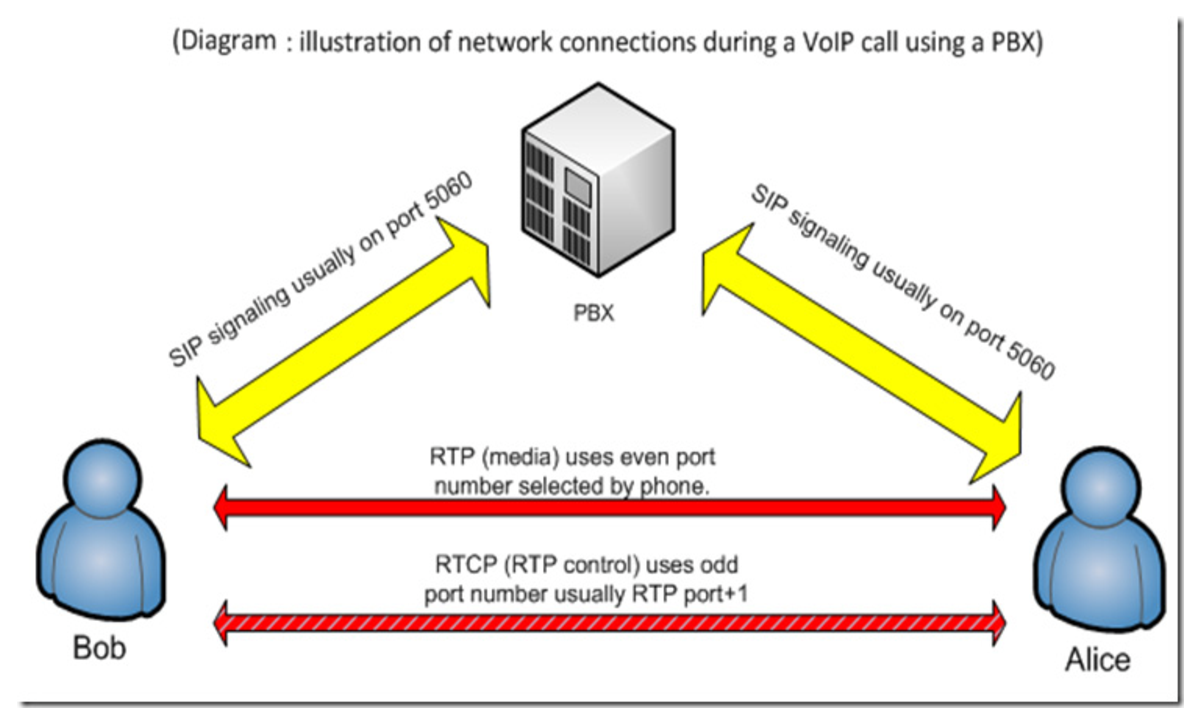
\includegraphics[width=0.9\linewidth]{images/rtp_sip}
\caption{How an RTP connection takes place for VoIP (image from \cite{rtp-sip})}
\label{fig:rtp-sip}
\end{figure}


Two flows are initialized : one for RTP and the other for RTCP. They usually use consecutive ports while RTP must use an even port number (\cite{RFC3550} Section 11). So only one pair of ports must be advertised for each host. This is only true for a unicast session. IP multicast can also be used with RTP and offer better performances if a large number of clients must access the same media resource. However, we won't give any details about how RTP multicast sessions are established since is it out of the scope of this thesis.

\subsection{RTCP}

RTP is just responsible for sending data to the receiver, with a little more information inside the packet than simple UDP. It includes sequence numbers, timestamps, information about the sources and control bits. But this mechanism alone does not give any hint about packet losses or the congestion of a link. This is why RTCP is essential in most of the applications.

According to \cite{javvin2005network}, RTCP performs four tasks : 

\begin{enumerate}
\item It provides feedback on the quality of the data distribution. It plays the role of a congestion control mechanism.
\item It carries an identifier for the RTP source called the canonical name. It allows each host to identify the participants in a particular flow. It can be useful when dealing with multicast.
\item It allows the source to compute the rate at which it has to send the packet. This takes into account the number of participants to the session.
\item It conveys minimal session control information, such as participant information to be displayed on user interface, for instance. This functionality is left optional.
\end{enumerate}

To do so, it carries Sender and Receiver reports. These reports are transmitted to the other party to estimate the quality of the link. They include information such :

\begin{itemize}
\item Packet count, octet count (received/sent)
\item Cumulative number of packets lost and fraction lost
\item Highest sequence number received
\item Different timestamps to estimate RTT and jitter.
\end{itemize}


\section{MPRTP}

Currently, RTP cannot support multipath because it operates at the session level and not at the transport level. Therefore RTP deals only with a particular media flow and not with the 5-tuple. The idea of MPRTP is to use multiple RTP flows concurrently on multiple interfaces. Figure \ref{fig:mprtp-concept} presents the system overview. As for RTP, the communication of the media is unidirectional : from a sender to at least one receiver. 


\begin{figure}
\centering
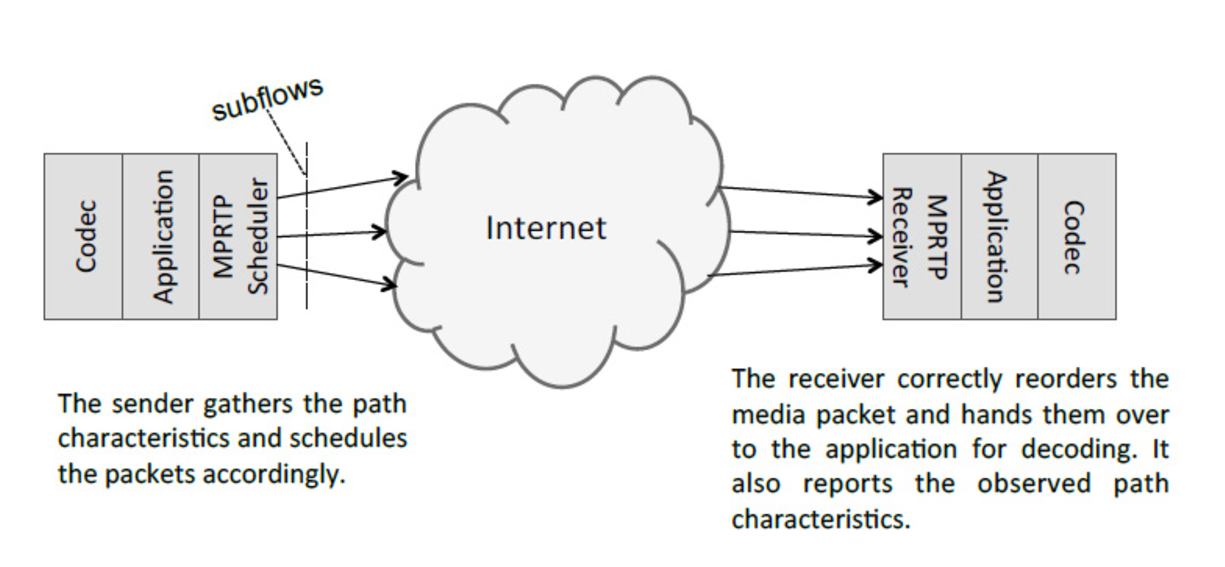
\includegraphics[width=0.9\linewidth]{images/mprtp}
\caption{MPRTP overview (taken from \cite{singh2013mprtp})}
\label{fig:mprtp-concept}
\end{figure}

\subsection{Design goals}

\subsubsection{Adapting to bandwidth changes}

If a link is congested, the scheduler must reduce the number of packets on this link and re-distribute the load among less congested links. But a small quantity of traffic must still be sent through this link just to monitor the link's characteristics (RTT, jitter). A similar approach is used in Multipath TCP \cite{wischik2011design}. Of course, the changes of repartition among the flows must be smooth and absorb small perturbations. Especially when used with mobile phones, the change of antenna may introduce a loss of connection on a very short period of time.

\subsubsection{Overcoming packet skew}

When you use disjoint paths over the Internet, you will likely encounter different delays. As a consequence, the packets will arrive out of order. To solve this problem, you need a large enough buffer at the receiver side. For multimedia communications, this is critical, as you want your song or video to be read in-order. While the problem can exist with DTLS, the constraint is less critical since the application must cope with out-of-order packets and implement by itself a buffer if needed. However, the scheduler could take care of carefully selecting the flow in order to minimize the skew.

\subsubsection{Choosing transmission paths}

Among the available paths, the MPRTP implementation must choose a subset of them to send the packets. This choice is actually an optimization problem based on multiple parameters. An endpoint may chose to optimize some of them. Following the scenario and the application needs, the scheduler may minimize losses, minimize latency or maximize end-to-end capacity.

\subsection{Getting subflow information}

To meet these goals, a scheduler will need to have information about the different sub-flows. Thanks to the sender and receiver reports from RTCP, MPRTP already have information about the complete session. However to get per-subflow information, it introduces RTCP per-subflow reporting. In order to decouple the subflow from the session, a subflow ID is assigned to each subflow. A flow is considered unique if the source and destination IP addresses and ports are different, which, together with the protocol, gives a 5-tuple.

To get an estimation of the packet jitter, packet loss and packet discard for a specific subflow, a subflow-specific sequence number is introduced. This new sequence number and the subflow ID are both carried in a header extension. This additional header is standardized in \cite{RFC3550} and will therefore allow backward compatibility.

Note that we don't have such tools in DTLS to evaluate a link's characteristics. We have build our own mechanism of feedback which is a simplified version of the sender and receiver reports of RTCP. More details are given on Section \ref{sec:mpdtls-feedback}. This extension has been designed without the multipath aspect in mind and thus could be implemented separately from MPDTLS.

\subsection{Addresses advertisement}
\label{sec:mprtp-advertise}

To establish new paths, a mechanism must advertise the addresses to the other host. In MPRTP, the choice is currently \cite{singh-avtcore-mprtp} left to the application to use in-band or out-of-band communication to take care of it.

\addtypes{byte, uint16}
\begin{lstlisting}[caption=MPRTCP Interface Advertisement, label=lst:mprtcp-advertisement]
struct {
   byte MPRTCP_Type;
   byte block_length;
   uint16 RTP_port;
   byte InterfaceAddress[(block_length-1)*4];
 } MPRTCPInterfaceAddress;
\end{lstlisting}

We focused on in-band communication since that is the way we choose to do it in our proposed design (see Section \ref{sec:advertise}). The MPRTCP extension for interface advertisement is defined in \cite{singh-avtcore-mprtp} sec. 9.3. The structure used to carry one particular IP address and port is shown on Listing \ref{lst:mprtcp-advertisement}.

The \texttt{MPRTCP\_Type} indicates the type of interface address. For now, 3 types are defined: 
\begin{enumerate}
\item IPv4 address
\item IPv6 address
\item DNS name
\end{enumerate}

The \texttt{block\_length} is the size of the block (i.e. the whole structure) in words of 32-bit. For an IPv4 address it should be 2 (1 for the interface itself and 1 for the information before), for an IPv6 it should be 5 and for a DNS name it will be variable.

The \texttt{RTP\_port} must be a valid RTP port number different from 0. The \texttt{InterfaceAddress} contains the actual IP address and its size is determined by the \texttt{block\_length}.

Note that Listing \ref{lst:mprtcp-advertisement} only presents the block to advertise one interface but such blocks will be combined in a unique packet to take into account multiple interfaces.

As stated in the working draft, all the interfaces in use must be transmitted. Moreover an endpoint must advertise its interfaces whenever an interface appears or disappears and when it receives an Interface Advertisement. We will use a similar strategy for MPDTLS. The fact you have to reply to an Interface Advertisement provides somehow an acknowledgment mechanism that could be useful in an unreliable protocol.

\subsection{Scheduling Algorithm}

The scheduler is one of the most important aspect and a critical point if you want the multipath approach to overcome the single path one. In the case of MPRTP, the sender must choose on which path to send the packets in order to guarantee a constant bit rate. A simple example with two paths is shown on Figure \ref{fig:mprtp-scheduler}.

\begin{figure}[!h]
\centering
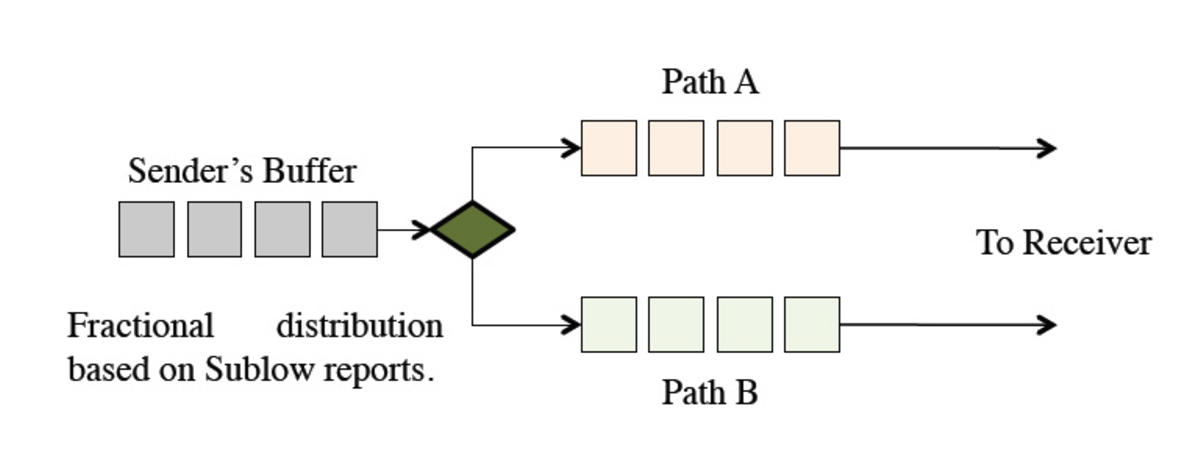
\includegraphics[width=0.9\textwidth]{images/mprtp-scheduler}
\caption{MPRTP Sender's Scheduler}
\label{fig:mprtp-scheduler}
\end{figure}

The goal of the scheduler is to compute the fractional distribution to distribute packets accordingly to paths characteristics. This means that a link with a smaller RTT will be probably given more load than another one.

However, the packets may arrive out-of-order if a significant difference in terms of RTT is noticed between paths. To compensate this reordering, a dejitter buffer must be set up at the receiver's side (Figure \ref{fig:mprtp-dejitter}). The buffer must be large enough to compensate variation in per path RTT.

\begin{figure}[!h]
\centering
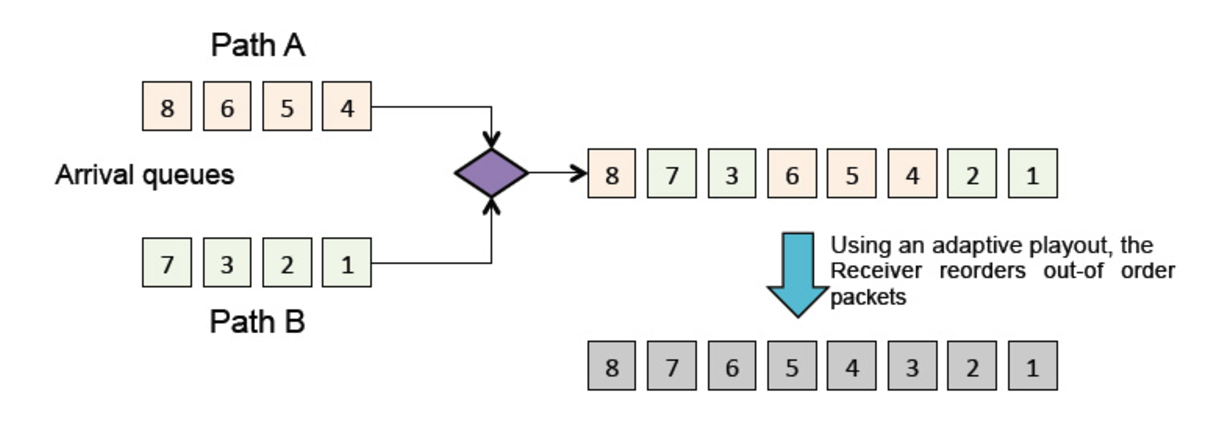
\includegraphics[width=0.9\textwidth]{images/mprtp-dejitter}
\caption{MPRTP buffer at receiver's side}
\label{fig:mprtp-dejitter}
\end{figure}

This buffer will rearrange the packets to put them in order and deliver the information to the application as a single stream.

\subsubsection{Receiver rate}

The receiver rate (RR) is computed for every flow as the total number of bytes that have been transiting through the flow between two consecutive receiver reports. This rate takes into account only the packets well received by considering the loss rate. When the receiver builds its $i^{th}$ report, the RR is computed as follow :

\begin{equation*}
RR = \frac{(\sum_{k = HSN_{i-1}}^{HSN_i} sizeof(X_k)) \times (1 - L_i)}{(t_i - t_{i-1})}
\end{equation*}

Where $HSN_i$ stands for the "Highest Sequence Number" received in the report $i$. So the sum actually represents the total number of bytes sent between two consecutive receiver reports. $L_i$ is the loss rate reported for this period of time.

\subsubsection{Calculating the fractional distribution}

The computation of the fractional distribution is not done each time the sender receives a receiver report. An interval timer is instead defined to do it more or less frequently following the network information. This interval expressed in seconds is computed as follow : 

\begin{equation*}
\begin{split}
SchInt & = \lambda \times S_{interval},\quad 0.5 \le \lambda \le 1.5 \\
 \lambda & = 0.5 + Rand(0.0,1.0)
\end{split}
\end{equation*}

The randomisation factor $\lambda$ is used to prevent multiple senders using the same paths to launch the computation as the exact same time. This would lead to a delta in server load. $S_{interval}$ is a value between the minimum and maximum RTCP interval [32,39]. It will be kept small at the beginning of the communication to recompute the distribution more frequently but progressively increases to the maximum. If congestion is detected, the $S_{interval}$ is reduced to recover quickly if the link becomes non-congested later on.

After the end of the interval, the distribution needs to take into account the state of each link in terms of congestion. For this purpose, three categories are defined : congested, mildly-congested and non-congested. To determine the category of one particular flow, the rules defined in \cite{ietf-avtcore-rtp-circuit-breakers} are used. This Internet draft aims at providing concrete rules to determine if a RTP application must stop sending packets to avoid congestion.

The proposed algorithm to split the traffic among all available paths will take into account the degree of congestion and will reduce the load of congested links.

\begin{align*}
SB[i] & = min\left( \frac{RR[i]}{\sum_{m} RR[m]} \times MR,\quad \alpha \times RR[i] \right) &\quad \text{if congested} \\
SB[i] & = min\left( \frac{RR[i]}{\sum_{r} RR[r]} \times MR,\quad \beta \times RR[i] \right) &\quad \text{if mildly-congested} \\
SB[i] & = \left( \frac{RR[i]}{\sum_{w} RR[w]} \times (MR - AP) \right) & \quad \text{if non-congested}
\end{align*}

Where $SB[i]$ is the sending bit rate for a particular path $i$, MR is the media rate (i.e. total bit rate) and $AP$ is the allocated bit rate. The indexes $m,r,w$ are used to represent the set of paths congested, mildly-congested and non-congested respectively. The minimum function is here to limit the maximum usage of a congested link but will not change anything if the link is already underused. Of course, this should be repeated for every path $i$.

The parameters $\alpha$ and $\beta$ must be tuned by experiments. In section 5.1 of \cite{singh2013mprtp}, $\beta$ is set to $0.8$ and $\alpha$ to $0.5$ after a series of tests in various configurations. These values make the scheduler reach the optimum fractional distribution quicker than other values.
\fi

\chapter{DTLS}\label{chap:dtls}


\section{Overview}

DTLS (Datagram Transport Layer Security) is a protocol designed to communicate securely over UDP. It was first presented in \cite{modadugu2004design} by Modadugu and Rescorla as an adaptation of TLS for delay sensitive applications. The objective was to be as close as possible from TLS while working as secure over an unreliable transport protocol. Like TLS, this protocol operates at level 5 in the OSI model (session layer). Therefore, the operating system does not provide any support for the protocol and every application has to manage it by itself. Typically, it implies either reinventing the wheel or using an existing library such as OpenSSL\footnote{\url{https://www.openssl.org/}}.

The current version of this protocol is DTLS 1.2 described in RFC6347 \cite{rfc6347}. Our work is based on this version because no effort concerning a possible version 1.3 has been recently noticed. We may expect such a version will come after the discussions on TLS 1.3 that are taking place as we are writing these lines. For now, the suggested modifications have no impact on our current design as we explain in Section \ref{sec:tls13impact}.

Even if this protocol is standardized for some years, only few important applications are using it. In the open source world, OpenVPN has planned to use it when UDP is used. Unfortunately, it seems not to be a top priority and they are still using a homemade protocol to do TLS over UDP. For commercial applications, we have only heard about Cisco AnyConnect \cite{anyconnect}. It is a VPN client to be used with Cisco servers. Although the sources of AnyConnect are not available, a open source project is born from this application: OpenConnect\footnote{\url{http://www.infradead.org/ocserv/index.html}}.

Nevertheless, some people are working actively to make DTLS a default transport protocol when dealing with application level communications. More details about potential use cases are given in Section \ref{sec:dtls-usage}.

\subsection{Objectives}

Like TLS, DTLS has 3 strong requirements: authenticity, integrity and confidentiality.

\subsubsection{Authenticity}

We speak about authenticity when one host is able to verify that the messages are coming from another known host. Therefore, someone cannot pretend he is the sender of packets as the receiving host will detect it.

\subsubsection{Integrity}

The integrity is guaranteed if the information carried cannot be altered without being detected. As a consequence, someone between the communicating hosts cannot add, remove or modify a single bit without the hosts finding it out.


\subsubsection{Confidentiality}

Confidentiality assures that a non-authorized entity will not be able to extract an understandable content from a message. Thus, it is not sufficient to capture a conversation to get the information.

\section{Foundations}

In this section we present the way of working of DTLS and its roots. We will start with a reminder of TLS goals and principles since it is strongly related. Then, we will go through the major differences between these two protocols. Finally, we will list the steps of a typical connection and present the different messages involved.

\subsection{TLS}
\label{sec:tls}

TLS is a protocol designed to provide a secure connection over reliable transport. It takes place between a server and a client.

Once the channel is established :
\begin{itemize}
\item The client has authenticated the server (i.e. the server is really the one he pretends to be\footnote{Under the assumption that the certificates can be verified by a reliable certification authority. It is the role of the Public Key Infrastructure (PKI) to provide and verify the certificates.}) and optionally vice-versa.
\item All messages can only be read by the other host (an eavesdropping is possible but the clear text cannot be obtained)
\item The packets cannot be replayed or modified on the line without the host finding it out.
\end{itemize}

To achieve these points, cryptography is used between both hosts and the packets are authenticated. TLS authentication typically uses cryptographic signature based on public key together with a certification authority. During the handshake, the two hosts are negotiating which version of protocol will be used together with algorithms to encrypt and authenticate the future messages. Many algorithms can be used to exchange the keys over an insecure channel. The two most common algorithms for key exchange are RSA and Diffie-Hellman.

The first one suffers from a lack of the perfect forward secrecy property. As stated in \cite{diffie1992authentication}, the perfect forward secrecy is guaranteed if the disclosure of long-term secret keying material does not compromise the secrecy of the exchanged keys from earlier runs. In the case of RSA, if an attacker has recorded entirely some sessions and then discovers the server's private key, she is able to determine the symmetric keys used for every session. Moreover, in the discussions about the incoming TLS 1.3 standard, an agreement was reached to remove RSA key transport in this version\footnote{\url{https://www.ietf.org/mail-archive/web/tls/current/msg12266.html}}. Note that RSA can still be used to provide the digital signatures since they are only needed during a short moment and will not reveal information about the content itself if the keys are compromised.

An alternative to RSA is the Diffie-Hellman (DH) algorithm for key exchange described in \cite{diffie1976new}. The original approach used large prime numbers and the modular arithmetic to generate the master key. Nowadays, it is more common to use the elliptic curve approach since it allows to generate keys of smaller size than standard approach without decreasing the security level. In addition, to achieve perfect forward secrecy, the algorithms deal with ephemeral keys meaning that the DH parameters are different for every session. This leads to two well known algorithms : DHE (Diffie-Hellman ephemeral) and ECDHE (Elliptic Curve Diffie-Hellman ephemeral).

From this point, we will consider ECDHE for key exchange and RSA for signatures. Figure \ref{fig:tls_handshake} illustrates TLS handshake with this configuration. The figure is taken from Cloudfare, a CDN\footnote{Content Delivery Network} provider. The visitor is the client and Cloudfare could be any TLS ECDHE compatible server. 

\begin{figure}[!ht]
\centering
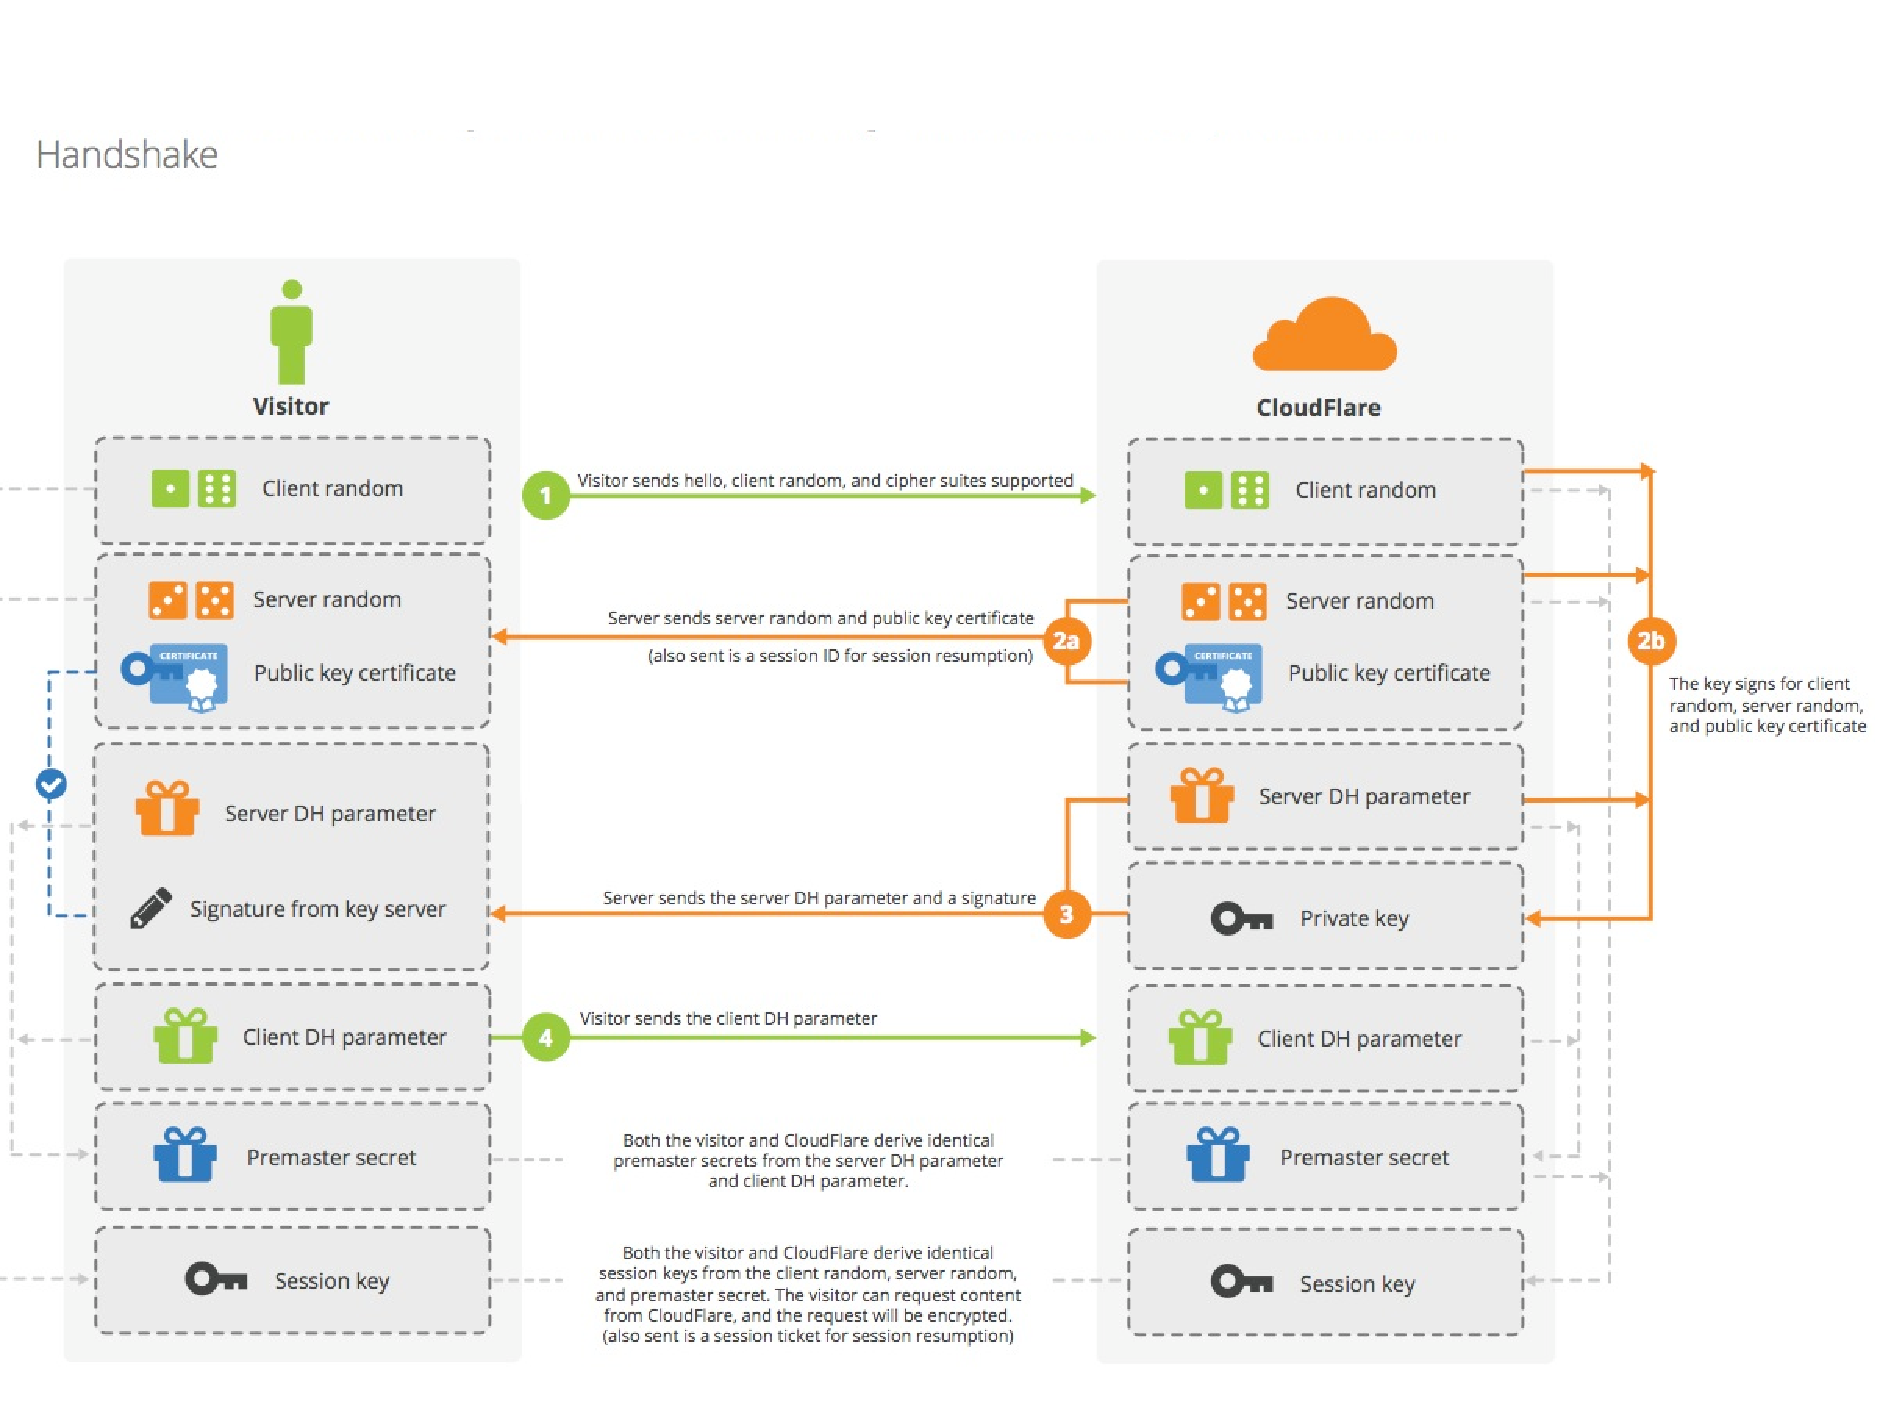
\includegraphics[width=\linewidth]{images/ECDHEhandshake}
\caption[TLS handshake with ECDHE]{TLS handshake with ECDHE for key exchange (image from \cite{tlsdhhandshake})}
\label{fig:tls_handshake}
\end{figure}

In the first phase, the client gives its version together with a list of algorithms for encryption and authentication called cipher suites. The client also gives to the server a random token to be used later. The server will then choose among the ones proposed: the version and the cipher suite to be used for the rest of the communication. A random server token is also included in the reply. In addition, the server may provide a session ID which can be used later for session resumption.

In a separated message, the server also provides its certificate to the client. It contains enough information for the latter to be able to verify server's identity. The certificate is generally emitted by a certification authority which is known by the client.

The next step comes with the server providing its DH parameters. In the case of ephemeral keys, the DH parameters must be different for every session. A digital signature using RSA with the server's private key is also included. The signature is computed not only on the information carried in this packet but also on all the previous exchanged messages. This is needed to prevent a man-in-the-middle attack. The genuine server is supposed to be the only one to hold the private key.

Then, the client provides its own DH parameters. Note that no signature is provided in this case as it is only optional to authenticate the client. Indeed, in some applications such as websites, this is not a requirement. After this step, both client and server can deduce the \textit{PreMasterSecret} and thus the master key with the random tokens exchanged before.

All messages following the handshake (containing application data) will be encrypted with symmetric cryptography using the keys deduced from the master key for this particular session. This will ensure the confidentiality. The two other objectives, authenticity and integrity of the messages, are ensured by a keyed-hash message authentication code (HMAC). It is generated as a hash on the content of the packet but the hash algorithm also integrates the secret key. Any cryptographic hash function can be used for this purpose but it is recommended to use at least \texttt{SHA256}. The choice of this function is also negotiated during the client hello, server hello phase. Even if it is better to first encrypt and then MAC the output as stated in \cite{bellare2000authenticated}, TLS works in reverse order for historical reasons. Currently people think it was a very bad idea from a security point of view and a RFC \cite{rfc7366} was published last year to push for the adoption of the encrypt-then-MAC technique on existing systems. It will probably be part of the TLS 1.3 RFC \cite{draft-tls13} to switch definitely to this better practice.

To prevent malicious replays disturbing the normal communication, TLS authenticates each packet with the associated sequence number. The sequence number is incremented for every packet sent but separately for each direction. Therefore each host has two counters: one for the packets sent and a second one for the packets received.

Thanks to a reliable transport protocol, these counters must never be transmitted explicitly because each host can compute them. As a consequence, if an attacker tries to replay packets, they will simply be rejected because the HMAC will not match with the most recent sequence number.

\subsection{Differences between TLS and DTLS}

\subsubsection{Unreliability}

The unreliability brought by UDP causes problems if we apply TLS over datagrams without any modification.

As we explain in the previous section, TLS uses implicit sequence numbers to authenticate packets. If a loss or a reordering occurs, then the sequence number considered by the receiving host will be wrong and the integrity check will fail. To solve this problem, DTLS modifies the record layer and adds a new field to carry the sequence number in every packet. The DTLS 1.2 record layer is presented on Listing \ref{lst:dtls-record}.

\addtypes{ContentType, ProtocolVersion, uint16, uint48, opaque}
\begin{lstlisting}[caption=DTLS record layer, label=lst:dtls-record]
struct {
   ContentType type;
   ProtocolVersion version;
   uint16 epoch;                                    // New field
   uint48 sequence_number;                          // New field
   uint16 length;
   opaque fragment[DTLSPlaintext.length];
 } DTLSPlaintext;
\end{lstlisting}


Epoch is used by endpoints to identify the keys used to protect the payload. The epoch is incremented by one once a \texttt{changeCipherSpec} is sent. Initially, the epoch is set to 0 for the handshake and the following \texttt{changeCipherSpec} will be the first message being part of the next epoch. The sequence number is set back to 0 once a new epoch has started. Due to the risks of retransmission or reordering, the endpoint need a way to know which set of keys were used to crypt the payload, because it cannot simply assume it is the latest negotiated keys. This need is fulfilled thanks to the epoch field.

Another problem raised by unreliability is the fact that in TLS the handshake has to follow a particular order and if not the connection is simply aborted. This is clearly incompatible with losses and retransmissions. To handle potential losses in the handshake phase, implementation must retransmit the last packet after a given time if no answer has been received from the other host (see \cite{rfc6347} Section 4.2.4).

To deal with possible reordering, all handshake messages have a given sequence number. So if a message is received before another one, the first message must be queued for further processing.

\subsubsection{Messages size}

The message size is a potential issue because TLS (and thus DTLS) messages can be as large as $2^{24}-1$ bytes while UDP datagrams are often limited to $1500$ bytes. Therefore, each DTLS handshake message may be fragmented over several DTLS records and then rebuilt. One fragment must fit in a single IP datagram to avoid IP fragmentation.

The benefits to this requirement are stated in the original DTLS paper \cite{modadugu2004design} :
\begin{itemize}
\item The DTLS layer does not need to buffer partial records, host memory can be used more efficiently.
\item It is quite possible that datagrams carrying the remaining record fragments are lost, in which case the received fragments are useless and cannot be processed.
\item Buffering record fragments would unnecessarily complicate a DTLS implementation without providing any obvious benefit.
\end{itemize}

Note that even if IP fragmentation occurs, DTLS will still operate correctly on top of re-assembly since it is transparently handled by the kernel.

The TLS handshake message is modified as shown on Listing \ref{lst:dtls-handshake}. The handshake message following this structure is also encapsulated into the record layer presented on Listing \ref{lst:dtls-record}.

\addtypes{HandshakeType, uint16, uint24, case, select}
\begin{lstlisting}[caption=DTLS handshake message, label=lst:dtls-handshake]
   struct {
     HandshakeType msg_type;
     uint24 length;
     uint16 message_seq;                               // New field
     uint24 fragment_offset;                           // New field
     uint24 fragment_length;                           // New field
     select (HandshakeType) {
       case hello_request: HelloRequest;
       case client_hello:  ClientHello;
       case hello_verify_request: HelloVerifyRequest;  // New type
       case server_hello:  ServerHello;
       case certificate:Certificate;
       case server_key_exchange: ServerKeyExchange;
       case certificate_request: CertificateRequest;
       case server_hello_done:ServerHelloDone;
       case certificate_verify:  CertificateVerify;
       case client_key_exchange: ClientKeyExchange;
       case finished: Finished;
     } body;
   } Handshake;
\end{lstlisting}

\subsubsection{Anti-Replay strategy}

In TLS, sequence numbers follow sequentially and a packet cannot be replayed because the HMAC verification will fail immediately. Such a drastic solution cannot be applied in DTLS because reordering or losses may occur. The DTLS 1.2 RFC \cite{rfc6347} sec. 4.1.2.6 describes the procedure to avoid replay using a sliding window. This strategy considers packets as valid even if they have been delayed or reordered while they are relatively close from the latest packets received. At the same time, the implementation must remember the packets received inside the sliding window and silently discard the replayed packets. Therefore, the MAC verification will only be done if the packets have not been received before, otherwise an undesirable packet is discarded at the record layer stage.

\subsubsection{Anti-DoS for the handshake}

In order to prevent DoS (Denial of Service) attacks, DTLS adds an additional step in comparison with the TLS handshake. Indeed, an attacker could send a lot of \texttt{ClientHello} messages and the server will have to keep a state for each of them, rapidly increasing the memory needed. Instead, the first \texttt{ClientHello} will not directly trigger a \texttt{ServerHello} but a \texttt{HelloVerifyRequest}. This message only carries the protocol version and a cookie as presented in Listing \ref{lst:dtls-helloverify}. This cookie must be retransmitted in the next Client Hello message. As we can seen on Listing \ref{lst:dtls-clienthello}, a new field has effectively been added to the \texttt{ClientHello} message.

\addtypes{ProtocolVersion, opaque}
\begin{lstlisting}[caption=DTLS HelloVerifyRequest message, label=lst:dtls-helloverify]
struct {
 ProtocolVersion server_version;
 opaque cookie<0..2^8-1>;
} HelloVerifyRequest;
\end{lstlisting}


\addtypes{ProtocolVersion, opaque, Random, SessionID, CipherSuite, CompressionMethod}
\begin{lstlisting}[caption=DTLS ClientHello adapted message, label=lst:dtls-clienthello]
struct {
 ProtocolVersion client_version;
 Random random;
 SessionID session_id;
 opaque cookie<0..2^8-1>;                             // New field
 CipherSuite cipher_suites<2..2^16-1>;
 CompressionMethod compression_methods<1..2^8-1>;
} ClientHello;
\end{lstlisting}

The additional \texttt{HelloVerifyRequest} message is also a counter measure against amplification attacks. Such attacks are trying to redirect traffic to overload a particular target by using an other server to generate bigger messages. These attacks are possible if the generated message is larger than the one triggering it. It is the case with DNS since the reply is larger than the request if a particular domain has multiple DNS records. It becomes then a vector for DoS attacks (see Figure \ref{fig:amp_attack} taken from \cite{dns-amp}).


\begin{figure}[!ht]
\centering
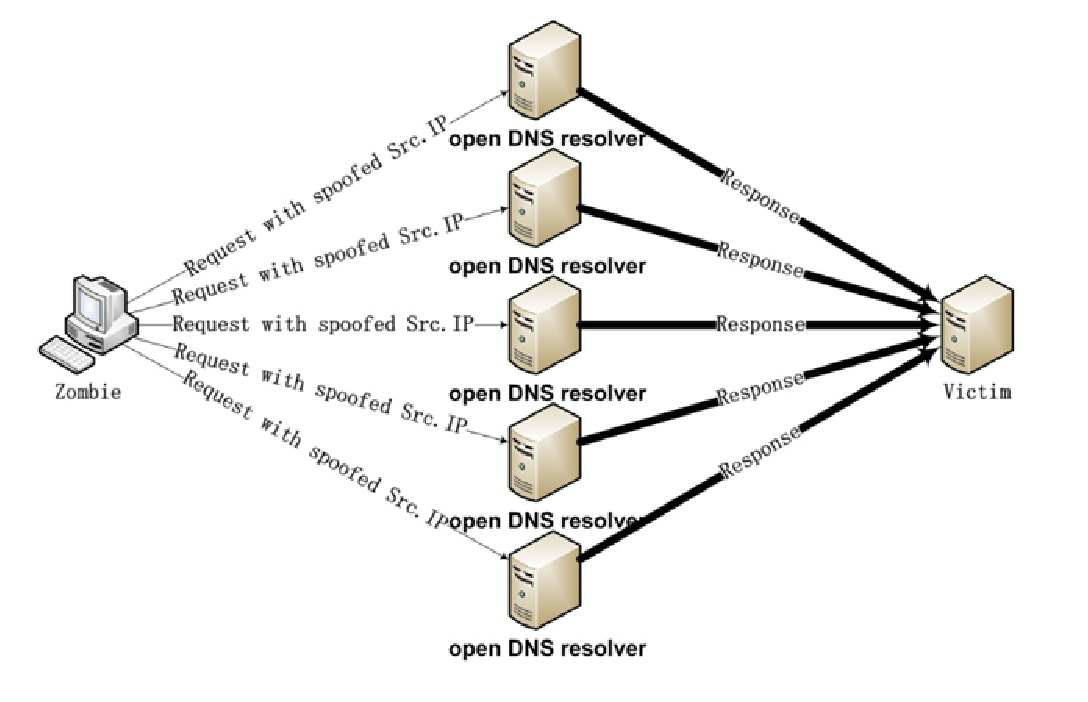
\includegraphics[width=\textwidth]{images/amplificationattacks}
\caption{Example of amplification attack with DNS}
\label{fig:amp_attack}
\end{figure}

For DTLS, the \texttt{ServerHello} is not larger than the \texttt{ClientHello} but amplification attack could still be possible (without the \texttt{HelloVerifyRequest}). Indeed, other messages are sent together with the \texttt{ServerHello}, including the one carrying the certificate (that could be quite large). Therefore, the additional step introduced with the \texttt{HelloVerifyRequest} (which is relatively small) prevents this kind of attack because the client has to prove it can answer at this address.

When the client sends its first \texttt{ClientHello}, the cookie field is initially empty. The server will then generate a new cookie which allows for a stateless exchange. It sends the \texttt{HelloVerifyRequest} with the cookie and doesn't remember anything about the client\footnote{This is indeed an exception to the retransmission measures. A \texttt{HelloVerifyRequest} will never be retransmitted, the client must first send another \texttt{ClientHello}.}. The DTLS server must generate cookies in such a way that they can be verified without retaining any per-client state on the server. A way to compute it is given in the RFC6347 section 4.2 \cite{rfc6347}:

\begin{lstlisting}
Cookie = HMAC(Secret, Client-IP, Client-Parameters)
\end{lstlisting}

The \texttt{Secret} is random and generated by the server. It could be periodically refreshed to invalidate previous cookies. Once a \texttt{ClientHello} has been received with a cookie, the server recomputes it and if both match, the connection can continue as in TLS with a \texttt{ServerHello} message.

\section{Typical DTLS communication}

\subsection{Handshake}

\begin{figure}[!h]
\centering
\begin{msc}[r]{DTLS Handshake}

\setlength{\instfootheight}{0em}
\setlength{\instheadheight}{0em}
\setlength{\instdist}{0.7\linewidth}
\setlength{\levelheight}{3em}

\declinst{client}{Client}{}
\declinst{server}{Server}{}

\mess{Client Hello}[t]{client}[0.3]{server}[1]
\nextlevel
\mess{Hello Verify Request}[t]{server}[0.3]{client}[1]
\nextlevel
\mess{Client Hello (w/ cookie)}[t]{client}[0.3]{server}[1]
\nextlevel
\mess{Server Hello}[t]{server}[0.5]{client}[1]
\nextlevel
\mess{Certificate}[t]{server}[0.5]{client}[1]
\nextlevel
\mess{Server Key Exchange}[t]{server}[0.5]{client}[1]
\nextlevel
\mess{Server Hello Done}[t]{server}[0.3]{client}[1]
\nextlevel
\mess{Client Key Exchange}[t]{client}[0.3]{server}[1]
\nextlevel
\mess{Change Cipher Spec}[t]{client}[0.3]{server}[1]
\nextlevel
\mess{Change Cipher Spec}[t]{server}[0.3]{client}[1]
\nextlevel
\nextlevel
\end{msc}
\caption{DTLS handshake with ECDHE-RSA cipher suite}
\label{fig:dtls-handshake}
\end{figure}


Figure \ref{fig:dtls-handshake} depicts a typical handshake with authentication of the server only and the ECDHE-RSA cipher suite\footnote{It means that Elliptic Curve Diffie-Hellman ephemeral is used for the key exchange and RSA for the signature.}. All messages before the \texttt{ChangeCipherSpec} are part of epoch 0. Their role is to negotiate the algorithms that will be used to compute the master key. The \texttt{Client Hello} has also the role to carry potential extensions supported by the client. If the server supports them as well, it will include them in the following \texttt{Server Hello} message. This is also where we chose to advertise our MPDTLS extension as explained in Chapter \ref{chap:design}.

The only difference with TLS (Section \ref{sec:tls}) is the presence of a second \texttt{ClientHello}. The first one is sent with no cookie and the second one must repeat the cookie received with the \texttt{HelloVerifyRequest}. Then the server confirms the cipher suite to be used through the \texttt{ServerHello} and directly sends its certificate and its ephemeral public key\footnote{In the case of ECDHE, it consists of the public DH parameters. Namely the domain parameters to define a particular curve.} including a signature of all previous exchanged messages. Finally the server sends the \texttt{ServerHelloDone} to explicitly say that the handshake is finished on its side.

Thereafter the client must also send its DH ephemeral public key. At this point, both parties have all the elements in their hands to compute the premaster secret. Note that unlike RSA, the secret is never communicated through the channel. With the random information exchanged through the \texttt{ClientHello} and \texttt{ServerHello}, each host can also compute the master key on its side. Consequently each peer will use this key to derive the set of keys used to communicate in the next epoch. The first messages of epoch 1 are the \texttt{ChangeCipherSpec} messages. They explicitly mark the separation between the handshake and the rest of the communication. Even if they are technically separated from the handshake, they are still considered as being part of it from a conceptual point of view.


\subsection{Application data}

Once the handshake has been completed, the peers can exchange Application Data packets. They are first encrypted and authenticated using the parameters negotiated earlier, then encapsulated into a Record Layer (Listing \ref{lst:dtls-record}).

DTLS doesn't bring any additional guarantee concerning the reliability of the link. As shown in Figure \ref{fig:dtls-data}, packets may be lost on the way and the application must deal with it. The sequence number for each message is indicated between chevrons. Sequence numbers are carried in clear inside the record layer, so each host knows how to verify the MAC and authenticate the packet.

\begin{figure}[!h]
\centering
\begin{msc}[r]{DTLS communication}

\setlength{\instfootheight}{0em}
\setlength{\instheadheight}{0em}
\setlength{\instdist}{0.7\linewidth}
\setlength{\levelheight}{3em}

\declinst{client}{Client}{}
\declinst{server}{Server}{}

\mess{Application Data <1>}[t]{client}[0.3]{server}[1]
\nextlevel
\mess{Application Data <1>}[t]{server}[0.3]{client}[1]
\nextlevel
\nextlevel
\lost[r]{Application Data<2>}[t]{}{client}[3]
\nextlevel
\mess{Application Data<3>}[t]{client}[0.3]{server}[1]
\nextlevel
\mess{Application Data<2>}[t]{server}[0.5]{client}[1]
\nextlevel
\nextlevel
\end{msc}
\caption{DTLS application data exchange}
\label{fig:dtls-data}
\end{figure}

\section{Use cases}

\label{sec:dtls-usage}

DTLS can be used almost everywhere UDP is used. We can think about applications such as VoIP (Voice over IP), multimedia, online gaming. Every application that wants to secure its communication but still benefit from faster transmission time of UDP may take advantage of using DTLS.

Of course the application has to cope with losses or reordering, but this is already the case for real time communication. As regards telephony, blank sounds replace the missing packets. For online gaming, high speed communication between the server and the client is needed to determine the character's position for instance. But if one packet is lost, the position can be determined by the next packet and the application will not be disturbed.

For video streaming applications, techniques are used to introduce a slight redundancy at the codec level in such a way that if some packets are lost, one frame may be missing but at least the video is still watchable\footnote{Of course, the application must a use a proper codec and compression method.}. It is also possible to introduce a small buffer to handle reordering.

In a recent Internet draft \cite{dtls-as-subtransport}, companies are trying to make DTLS the default sub-transport protocol for all application-level protocols when security is needed. This will raise DTLS to the rank of "good practice" for secured communications.

Another important use case for DTLS comes with its integration in WebRTC\footnote{\url{http://www.webrtc.org/}}. This is an open project which has an objective to bring real time communications to browsers and mobile applications via simple APIs. In this context, DTLS has been chosen to ensure the communication between two peers (i.e. browsers or mobile apps). The internet draft describing the security architecture of WebRTC \cite{ietf-rtcweb-security-arch} proposes to use SRTP over DTLS for multimedia communications and DTLS alone for any other kind of data. Figure \ref{fig:webrtc} is taken from a presentation \cite{rescorla2011proposed} made by E.Rescorla and shows how the connection is set up in this proposed design.  

\begin{figure}[!ht]
\centering
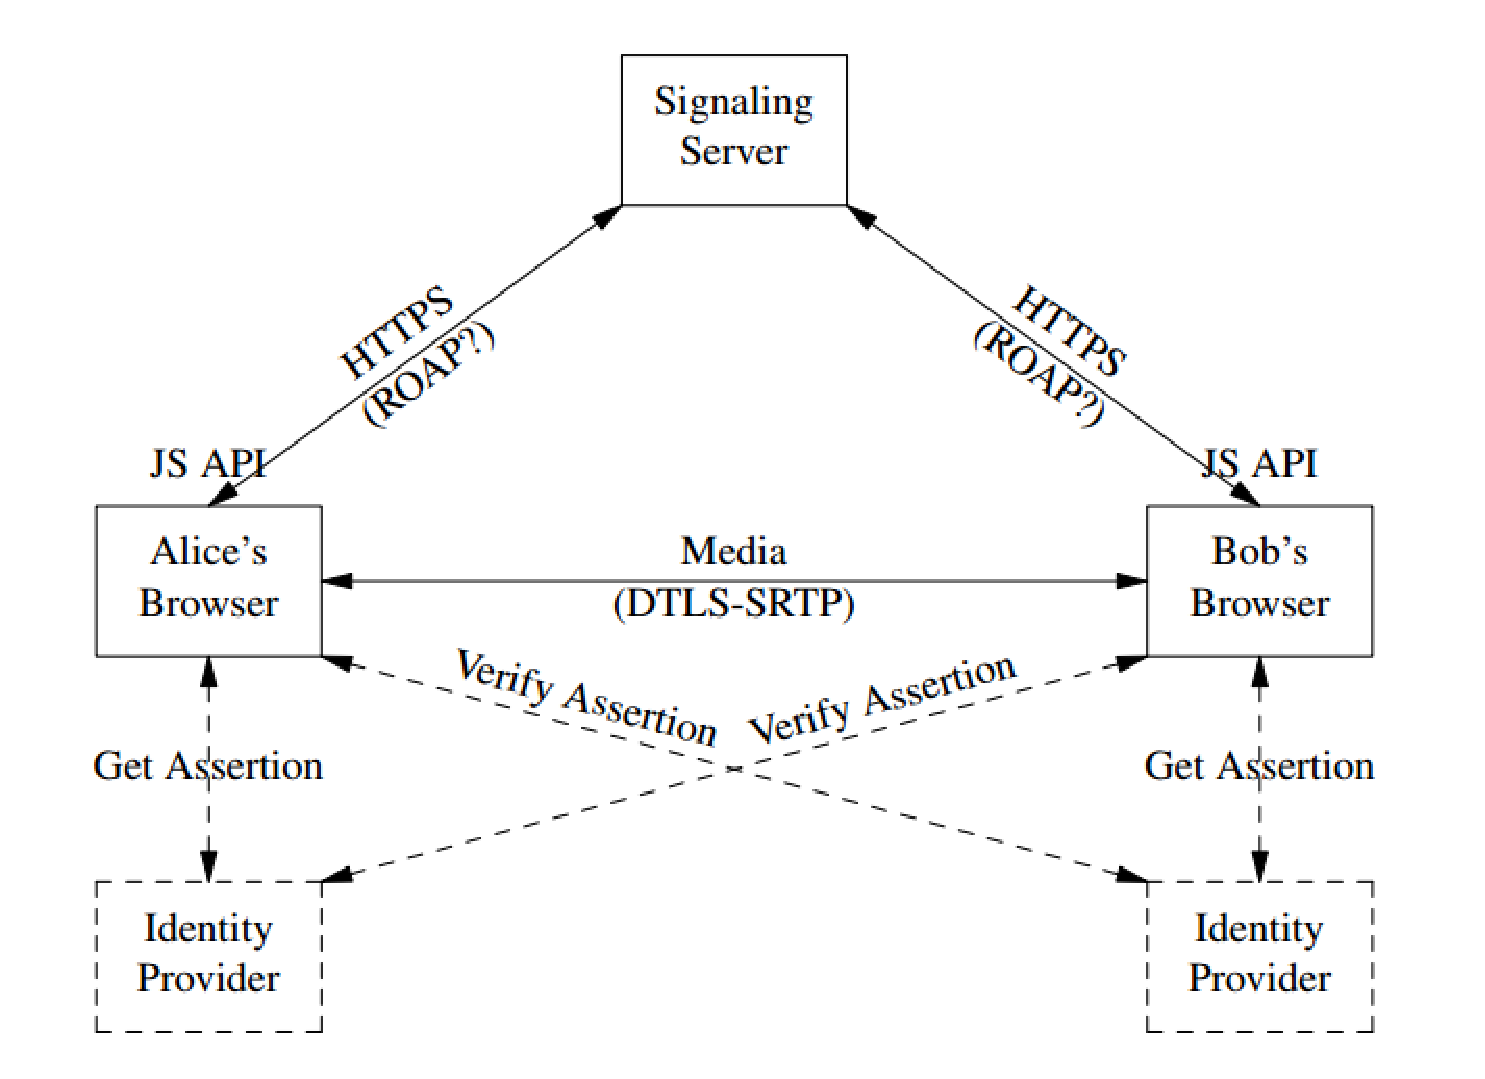
\includegraphics[width=0.9\textwidth]{images/webrtc.eps}
\caption{Proposed design for WebRTC security architecture}
\label{fig:webrtc}
\end{figure}

By the peer to peer nature of this application, a signalling server is needed to act as a "rendez-vous" point and to perform NAT traversal. Then the handshake can take place and identity providers issue and verify certificates. Finally all data are transmitted through the DTLS transmission and multiple SRTP sessions can use the same DTLS session. 

To sum up, all these applications may benefit from using DTLS but also MPDTLS as it will allow more resilience and better performances. We will demonstrate this point in the following chapters.

\section{Security considerations}
\label{sec:tls-sec}

Most of the security considerations are the same as those of TLS 1.2 \cite{RFC5246} since DTLS is only an adaptation of TLS for unreliable transport protocols.

The attacks known for TLS could theoretically be used for DTLS as well. This is the case for the "secure renegotiation". As a reminder, this vulnerability allows an attacker who can hijack a HTTPS connection to add custom request to a communication between the client and the web server. Even if the attacker cannot retrieve the content of the communication, it can still have dramatic consequences. As depicted on Figure \ref{fig:tls-reneg} taken from \cite{tls-reneg}, an attacker can inject bank orders and then trigger the renegotiation with a real client. The bank order is only delayed and when the renegotiation is completed, it is executed before anything else. The best solution up to know is to disable by default this feature or to implement the extension described in \cite{rfc5746}.

\begin{figure}[!ht]
\centering
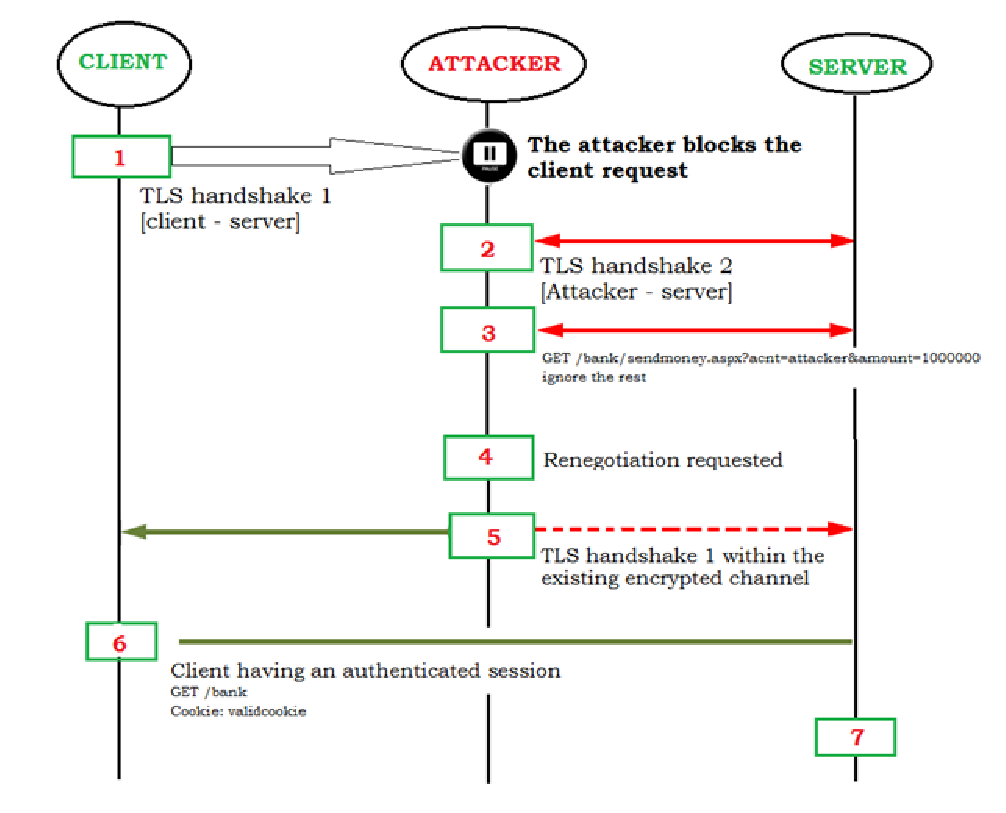
\includegraphics[width=0.8\textwidth]{images/TLSrenegotiation}
\caption{TLS renegotiation vulnerability}
\label{fig:tls-reneg}
\end{figure}

Other attacks could also be applied to DTLS and be more efficient on DTLS than on TLS, namely the DoS attacks. Two main categories can be identified :

\begin{itemize}
\item The blind DoS : packets are being transmitted with a spoofed IP address to redirect the traffic to another target (amplification attack) or to simply not diclose the IP address of the attacker. They are called blind because the attacker will never receive any answer from the server. They are made easier with UDP because no handshake is needed with the server.
\item Computational DoS : the attacker can reply to certain messages but will try to optimize the ratio between the work he has to do and the work he is asking to the server.
\end{itemize}

Blind DoS are made impossible in TLS because the attacker must first complete the TCP handshake and thus prove he can answer at this address. As presented earlier, the introduction of the \texttt{Hello Verify Request} will prevent this kind of attack for DTLS too.  Although it is not a strict requirement to implement this feature in DTLS (\cite{rfc6347} Section 5), it is strongly recommended for DTLS servers  unless there is a good reason to think that no amplification is possible in their environment.

Nevertheless the second type can still be used to disturb a server running DTLS or even TLS. As explained by E. Rescorla in \cite{tls-dos}, nothing is done at the design level to prevent these kind of attacks because it would imply putting a lot of work on the client side. It is generally a bad idea for performances. Moreover, the attackers are often using infected computers of casual people to launch DoS attacks. Therefore they have a lot of CPU power available anyway.

\section{Heartbeat extension}

The heartbeat extension is unfortunately known for the famous heartbleed bug\footnote{\url{http://heartbleed.com/}} detected in April 2014. Every server using OpenSSL at this time was vulnerable and part of the memory could be retrieved (including private keys, passwords\dots). It is important to note that the error came from the implementation of the extension inside OpenSSL and not from the standard itself.

Anyway, this extension can be really useful to assess the availability of a link and also provides a keep-alive feature. It is quite simple but it also allows for extensibility and new messages as stated in RFC6520 \cite{rfc6520}. The structure of a heartbeat message is presented on Listing \ref{lst:hb-msg}. This will take place on top of the Record Layer (Listing \ref{lst:dtls-record}). The advertisement of this extension is made through a Hello extension. It also defines the behavior of the hosts upon the reception of Heartbeat messages.

\addtypes{HeartbeatMessageType}
\begin{lstlisting}[caption=Heartbeat message, label=lst:hb-msg]
struct {
  HeartbeatMessageType type;
  uint16 payload_length;
  opaque payload[HeartbeatMessage.payload_length];
  opaque padding[padding_length];
} HeartbeatMessage;
\end{lstlisting}

For now, only two types of Heartbeat messages are in use : \texttt{Heartbeat Request} and \texttt{Heartbeat Response}. The response must contain the same payload as the one in the request triggering it. A simple exchange is presented on Figure \ref{fig:heartbeat}.

\begin{figure}[!h]
\centering
\begin{msc}[r]{Heartbeat request/response}

\setlength{\instfootheight}{0em}
\setlength{\instheadheight}{0em}
\setlength{\instdist}{0.7\linewidth}
\setlength{\levelheight}{3em}

\declinst{host1}{Host 1}{}
\declinst{host2}{Host 2}{}

\lost[r]{Heartbeat Request}[t]{}{host1}[3]
\nextlevel
\mess{Heartbeat Request}[t]{host1}[0.3]{host2}[1]
\nextlevel
\mess{Heartbeat Response}[t]{host2}[0.5]{host1}[1]
\nextlevel
\nextlevel
\end{msc}
\caption{Heartbeat requests and responses}
\label{fig:heartbeat}
\end{figure}

Other messages may be implemented since a new IANA section has been opened to register the different \texttt{HeartbeatMessageType}. Indeed, as you will see in the Chapter \ref{chap:implementation}, we have designed a new type of message used to transmit a timestamp.


\if0\draft
\chapter{Protocol Design}\label{chap:design}

In this chapter, we will explore the different additions and modifications made to DTLS to support the Multipath capability. These changes are categorized in three groups:
\begin{itemize}
\item Advertising the extension and the interfaces
\item Establishing secure sub-flows without introducing attacks vectors
\item Gathering and exchanging statistics data about the health of each flow, regardless of the others. 
\end{itemize}


\section{Multipath advertisement}

Our main purpose is to set up this protocol as an extension of DTLS. In this way, we can reuse as much as possible the principles established by Rescorla and Modadugu in \cite{modadugu2004design}. This also explains why we tried not to change the existing DTLS frames and to add instead new frames for new usages.

\subsection{Extension discovery}\label{sec:helloext}

The first step, and the first requirement, was to remain compatible with the standard DTLS client and server. To do that, the MPDTLS extension discovery is made through a new entry in the extensions list of the \texttt{ClientHello} and \texttt{ServerHello} messages. If a MPDTLS-unable server receives a \texttt{ClientHello}, it will ignore the option as it is specified in the TLS 1.3 specifications (\texttt{draft-ietf- tls-tls13}\cite{draft-tls13}). This option is carried as any other TLS Hello Extension (Section 7.3.2.5 from the same draft) with the following format:

\addtypes{ExtensionType, byte, Extension}
\begin{lstlisting}[caption=MultiPath DTLS Extension structure, label=lst:extension]
struct {
  ExtensionType extension_type;
  byte          extension_length[2];
  byte          extension_data[1];
} Extension;

enum {
    mpdtls_extension(TBD, 42 in dev), (65535)
} ExtensionType;
\end{lstlisting}

This extension is simply carrying a byte indicating if the host supports MPDTLS or not (so it carries \texttt{0x01} or \texttt{0x00} respectively).

After the exchange of the \texttt{HelloVerifyRequest} and \texttt{ClientHello} with Cookie, the server will send back a \texttt{ServerHello} containing the same extension if it wants to support MPDTLS features. Besides this MPDTLS extension discovery, the handshake is exactly the one from DTLS, keeping the handshake as light as possible.

\subsection{Advertising interfaces}
\label{sec:advertise}

Like in MPRTP (see Section \ref{sec:mprtp-advertise}), we can explore 2 options for the addresses advertisement : in-band or out-of-band signalling. "In-band" means we use the same protocol (in this case DTLS) to exchange our addresses while "out-of-band" will imply another protocol that could be reliable for instance. For MPDTLS, we made the choice to consider only the in-band communication for the following reasons : 

\begin{itemize}
\item Lower overhead: we don't need any additional protocol or to set up another channel of communication.
\item The addresses must be communicated securely. We already have a secure channel with DTLS, it is thus unnecessary to do another handshake with TCP/TLS.
\item The reliability is not a strong requirement. The message carrying all the addresses may be lost, this is not vital for the communication. Moreover, with a small retransmission strategy, it will eventually reach the destination.
\end{itemize}


Once the handshake is finished and the initial flow is established, the two hosts can advertise new interfaces available for other sub-flows. This is done within the \texttt{ChangeInterfaceMessage} (CIM), a packet carrying multiple addresses. This packet is carried as a DTLS fragment and thus is protected in the same way the Application Data are. The structure of the \texttt{CIM} packet is shown in the Listing \ref{lst:cimformat}. We use 16 bytes for the address to be IPv6 compliant. IPv4 addresses can be mapped to/from IPv6 format following \texttt{RFC4291}\cite{rfc4291}. This mapping allows us to keep the size of the packet relatively small when you compare it with the one from MPRTP (Listing \ref{lst:mprtcp-advertisement}). Of course we don't support DNS name. It could be interesting to let the other host do the DNS resolution but for now we think it is not needed. We can always extend the design if a need for other kind of interface advertisement is observed.

\addtypes{ContentType,ProtocolVersion,uint16,uint48,uint64,byte,ChangeInterfaceMessageFragment,DTLSPlainText, NewAddress,select,case}
\begin{lstlisting}[caption=Change Interface Message, label=lst:cimformat]
struct {
    ContentType type;
    ProtocolVersion version;
    uint16 epoch;
    uint48 sequence_number;
    uint16 length;
    select (ContentType) {
        case change_interface: ChangeInterfaceMessageFragment; // New field
    } fragment;
} DTLSPlaintext;

enum {
    change_interface(TBD, 42 in dev), (255)
} ContentType;

struct {
    byte reply;
    if (reply) {
        uint48 ack;
    }
    byte number_addresses[2];
    NewAddress addresses<1..2^16-1>;
} ChangeInterfaceMessageFragment;

struct {
    byte address[16];
    uint16 port;
} NewAddress;
\end{lstlisting}

The \texttt{CIM} contains all the addresses a host wants to share. We decided to always transmit all the addresses to provide redundancy. Also, to be sure we do not lose potential bandwidth, the \texttt{CIM}s are retransmitted in case of loss and so are acknowledged. To avoid wasting resources, we use the acknowledgement to transmit the list of addresses of the receiving host. This way, we are sure that each host knows the exact configuration of the other at any time (once the first host received the acknowledgement). This strategy has also been chosen for the retransmission in MPRTP \cite{singh-avtcore-mprtp}.

An example of the \texttt{CIM} exchange is shown in the Figure \ref{fig:CIMexchange}. The message is structured as follows: the fact that it is an acknowledgement or not (reply bit), the total number of interfaces we are advertising and the list of interfaces (following format presented in Listing \ref{lst:cimformat}). For the sake of clarity, the DTLS informations (such as the epoch, version,\dots) are not represented on Figure \ref{fig:CIMexchange} and the sequence numbers are shown between chevrons.

\begin{figure}[!ht]
\centering
\begin{msc}[r]{MultiPath-DTLS Addresses announcement}

\setlength{\instfootheight}{0em}
\setlength{\instheadheight}{0em}
\setlength{\instdist}{0.7\linewidth}
\setlength{\levelheight}{3em}

\declinst{client}{Client}{}
\declinst{server}{Server}{}

\lost[r]{ChangeInterfaceMessage[[reply=1], 2, client1, client2 ] - <1>}[t]{}{client}[8]
\settimeout{}{client}[1]
\nextlevel
\mess{ChangeInterfaceMessage[[reply=1], 2, client1, client2] - <2>}[t]{client}[0]{server}[1]
\nextlevel
\mess{ChangeInterfaceMessage[[reply=0,ack=2], 1, server1] - <1>}[b]{server}[1]{client}[1]
\nextlevel
\nextlevel

\end{msc}
\caption{Example of Change Interface Message use}
\label{fig:CIMexchange}
\end{figure}

To avoid an infinite exchange of \texttt{CIM}s, a reply bit is needed and placed into the header of \texttt{CIM} to differentiate a new message from an acknowledgement to a previous one. Also, to know which CIM request is acknowledged, its DTLS sequence number is added in the response. The client must store the sequence number of the last CIM emitted. When an \texttt{CIM} is received but the host realizes the stored sequence number doesn't match the received ack, it must retransmit the \texttt{CIM}.

\subsection{Retransmission strategy}

A CIM message must be retransmitted if the reply is not received because the packet may be lost. How do we monitor the reception ? We could use a timeout to retransmit after a certain period of time. But if the other host is definitely dead, we will send packets for nothing before we figure out.

We could point out the fact that the knowledge of the interfaces is only needed when the host is really using them (i.e. sending packets). Therefore, we could think of a mechanism which retransmits only when there is evidence that the other is still alive : when we receive application data packets. When the first CIM is sent, we set a flag to 1. This flag is put back to 0 as soon as we receive a CIM with \verb$reply = 0$. But if we receive an application data with the flag still on, we process the data and retransmit the last CIM. An example is presented on Figure \ref{fig:CIMexchange2}.

\begin{figure}[!ht]
\centering
\begin{msc}[r]{MultiPath-DTLS Addresses announcement RTX}

\setlength{\instfootheight}{0em}
\setlength{\instheadheight}{0em}
\setlength{\instdist}{0.7\linewidth}
\setlength{\levelheight}{3em}

\declinst{client}{Client}{}
\declinst{server}{Server}{}

\lost[r]{ChangeInterfaceMessage[reply=1, 2, client1, client2]}[t]{}{client}[7]
\nextlevel
\mess{ApplicationData}[t]{server}[0.3]{client}[1]
\nextlevel
\mess{ChangeInterfaceMessage[reply=1, 2, client1, client2]}[t]{client}[0.25]{server}[1]
\nextlevel
\mess{ChangeInterfaceMessage[[reply=0], 1, server1]}[b]{server}[1]{client}[1]
\nextlevel
\nextlevel

\end{msc}
\caption{Example of Change Interface Message Retransmission}
\label{fig:CIMexchange2}
\end{figure}

Of course if some packets were already on the line before the server has received the CIM, we will retransmit many times the CIM and therefore waste bandwidth.

Our solution is somehow a mix between the pure timeout and the direct retransmission after every packet. When we first send the \texttt{CIM}, we store a timestamp in a variable. For every packets received, we check if the elapsed time is enough and we retransmit the packet and reset the timestamp to the current time. The "enough" is customizable, we could set a default value of 2 RTT for \texttt{CIM} retransmission. The main benefit of checking only when we receive packets is that we don't waste bandwidth for dead links and we don't need parallelization mechanism (e.g. interruptions).

This strategy will be used for all retransmission of control packets with possibly different thresholds for the timers.

\section{Secure sub-flows setup}\label{sec:setupflow}

In the first design of our protocol, we didn't use any handshake to attach new sub-flows to the global connection. Instead, we were creating all the possible sub-flows by combining the host and remote addresses, directly initializing the sockets in connected mode. However, this solution is not suitable in various situations, like NAT-traversals or short-living interfaces. 

Other multipath protocols don't need to explicitly start a new flow. That's the case for MPRTP, the interfaces are just advertised and all possible combinations of 2 interfaces are then acceptable. But MPRTP doesn't have any security concerns as we do.

Using not connected sockets could present a potential weak point for a DoS (Denial of Service) attack. If an attacker could guess IP addresses of the server, she can send garbage under the form of traditional DTLS packets. This could get computation costly since it forces the server to establish the packet authenticity and involves cryptographic operations. This is cheaper if we use connected sockets because packets coming from other addresses or ports than the connected ones are immediately dropped by the UDP stack. Also, this problem does not appear when the involved packets are not cryptographically signed, like the handshake packets. The solution presented in the Section \ref{sec:breakbeforemake} allows to overlook this issue as it is based on the shortened DTLS handshake.

To address this issue, we define three scenarios of sub-flow creation and the solutions to cope with.

\subsection{Make-before-break sub-flows}
\label{sec:mbf}

We want to set up a new sub-flow when we have at least one other sub-flow alive. In this situation, we will use the secure communication already established to negotiate the opening of a new connection. Only when the negotiation is completed, a new socket will be created and connected on both side, avoiding any possible DoS attack on the new interface.

To carry this request, we need a new type of packet : \texttt{wantConnect}, whose structure is shown on Listing \ref{lst:WantConnect}.

\addtypes{WantConnectFragment}
\begin{lstlisting}[caption= WantConnect message, label=lst:WantConnect]
enum {
    want_connect(TBD), (255)
} ContentType;

struct {
    NewAddress addr_src;
    NewAddress addr_dst;
    byte opts;
} WantConnectFragment;

struct {
    byte address[16];
    uint16 port;
} NewAddress;
\end{lstlisting}

The field \texttt{opts} can be used to specify options for the incoming connection. The first bit of opts is telling if the host accepts or refuses the connection and will only be used in the reply. A second bit is used as the backup flag. When this flag is set to 1, it means we want to use this interface only if it is the only possible choice to keep the connection running. Typically, this would be the case for a 4G/LTE interface on a phone because it costs much more than the Wi-Fi. The 6 remaining bits are unused for now but may be useful in the future.

The host who received a \texttt{wantConnect} must acknowledge the reception thanks to a \texttt{wantConnect Ack} packet (see Listing \ref{lst:WantConnectAck}). Messages can be lost and we need to know to which Packet the acknowledgement is referring to, so we include the sequence number of the corresponding packet (i.e. DTLS sequence number). The options are also included to give the opportunity to the other host to accept or deny some of them. In particular, the first bit is set to 1 if the host refuses the connection and zero otherwise.

\addtypes{WantConnectAckFragment}
\begin{lstlisting}[caption= wantConnectAck message, label=lst:WantConnectAck]
enum {
    want_connect_ack(TBD), (255)
} ContentType;

struct {
    uint48 ack_seq;
    byte opts;
} WantConnectAckFragment;
\end{lstlisting}

Figure \ref{fig:Handshake1} presents how it will take place when a server has 2 interfaces and the client only one. First the traditional DTLS handshake is established between the client and the public interface of the server (S1). By a \texttt{CIM} exchange, the client is aware of the existence of a second interface (S2). He then sends a \texttt{wantConnect} request and if this message is correctly received, the server will set up his second interface to receive packets from the client. After this exchange, heartbeat messages will take place to assess the availability of the link. The frequency must be defined according to experimentation, at this point we recommend to send a heartbeat message at least every 5s. The implementation must use a back-off strategy to prevent waisting resources on a dead link. If for some reasons, the interface is not reachable from the client, then the server will find out it never receives any heartbeat response and will close the socket. Otherwise, a new sub-flow has been set up and both hosts can use it to communicate securely. 


\begin{figure}[!ht]
\centering
\begin{msc}[r]{MultiPath-DTLS handshake make-before-break}

\setlength{\instfootheight}{0em}
\setlength{\instheadheight}{0em}
\setlength{\instdist}{0.33\linewidth}
\setlength{\levelheight}{3em}

\declinst{client}{Client (C)}{}
\declinst{server1}{Server1 (S1)}{}
\declinst{server2}{Server2 (S2)}{}

\mess{DTLS Hanshake}[t]{client}[0.5]{server1}[0]
\nextlevel
\mess{DTLS Hanshake}[t]{server1}[0.5]{client}[0]
\nextlevel
\mess{CIM[2, S1, S2, reply=1]}[t]{server1}[0.1]{client}[1]
\nextlevel
\mess{CIM[1, C, reply=0]}[b]{client}[0.8]{server1}[1]
\nextlevel[2]
\mess{WantConnect[C,S2,op]}[t]{client}[0.1]{server1}[1]
\nextlevel
\mscmark{connected socket}{server2}
\mess*{}{server1}{server2}[0]
\mess{WantConnectAck[op]}[t]{server1}[0.3]{client}[1]
\nextlevel
\mscmark[br]{connected socket}{client}
\nextlevel
\mess{HeartbeatRequest}[t]{client}[0.6]{server2}[1]
\nextlevel
\mess{HeartbeatResponse}[b]{server2}[0.4]{client}[1]
\nextlevel[2]

\end{msc}
\caption{Example of new sub-flow establishment when another connection is alive}
\label{fig:Handshake1}
\end{figure}

When another connection is available, this is the best method to establish a new sub-flow since it is way faster than a complete handshake. Note that the two new messages introduced are secured as any other DTLS message and therefore cannot be forged or replayed.


\subsection{Break-before-make sub-flows\label{sec:breakbeforemake}}
Unfortunately, the solution presented in the previous section is not applicable in every situation; for instance, when a smartphone is connected with its Wi-Fi interface and the access point becomes out of range for any reason. The smartphone will then toggle the 4G interface. It cannot use the procedure explained in the previous section as it does not have an active sub-flow anymore. To solve this problem, the smartphone can simply use the Session Resumption mechanism available in (D)TLS, resuming on both sides the state of the session as before the link failure. It is also important that the smartphone warns the server that the Wi-Fi interface is no more available by sending a \texttt{CIM} as soon as it re-establishes the connection. This use case is presented on Figure \ref{fig:dtls-sessionresumption}.

\begin{figure}[!ht]
\centering
\begin{msc}[r]{MultiPath-DTLS session resumption}

\setlength{\instfootheight}{0em}
\setlength{\instheadheight}{0em}
\setlength{\instdist}{0.33\linewidth}
\setlength{\levelheight}{3em}

\declinst{client1}{Client2 (4G)}{}
\declinst{client2}{Client1 (WiFi)}{}
\declinst{server}{Server}{}

\mess{DTLS Hanshake}[t]{client2}[0.5]{server}[0]
\nextlevel
\mess{DTLS Hanshake}[t]{server}[0.5]{client2}[0]
\nextlevel
\mess*{Share session ID}{client2}{client1}[0]
\nextlevel
\condition{WiFi Off}{client2}
\nextlevel
\stop{client2}
\condition{4G On}{client1}
\nextlevel
\mess{ClientHello (with session id)}[t]{client1}[0.5]{server}[0]
\nextlevel
\mess{HelloVerifyRequest}[t]{server}[0.5]{client1}[0]
\nextlevel
\mess{ClientHello (with session id, cookie)}[t]{client1}[0.5]{server}[0]
\nextlevel
\mess{ServerHello (with same session id)}[t]{server}[0.5]{client1}[0]
\nextlevel
\mess{ChangeCipherSpec}[t]{server}[0.5]{client1}[0]
\nextlevel
\mess{ChangeCipherSpec}[t]{client1}[0.5]{server}[0]
\nextlevel
\mess{ChangeInterface(Client2)}[t]{client1}[0.5]{server}[0]
\nextlevel
\mess{ChangeInterface(Server)}[t]{server}[0.5]{client1}[0]
\nextlevel[2]

\end{msc}
\caption{Example of how session resumption takes place}
\label{fig:dtls-sessionresumption}
\end{figure}

Note this is only possible because Client1 and Client2 are the same machine and therefore share the session ID given by the server. The handshake is faster if the session is still on the server's cache because no certificate exchange is needed and the master key is the same as before.

This solution presents the same security properties than the standard Session Resumption proposed in the \texttt{RFC5246}\cite{rfc5246}, Section 7.4.1.2. The RFC doesn't explicitly limit the session resumption to come from the same IP/port as before but it appears that some implementation do it. It was the case for Firefox and was criticized as a bug by N. Modadugu who is the co-author of DTLS\footnote{\url{https://bugzilla.mozilla.org/show_bug.cgi?id=415196}}. It can't be considered as a weakness since even if an attacker can steal the session ID, he doesn't know the master key and therefore won't be able to generate a correct \texttt{ChangeCipherSpec}.

If the server clears the session cache in the meantime, the full DTLS handshake will take place and the server and the session will start without any other known remote interface. This is another reason to impose a \texttt{CIM} emission as soon as the sub-flow is up.

Moreover, to make this solution working, a thread or a process must be constantly listening the interface even if a connection is already initiated. This was not a requirement for the \textit{WantConnect} solution.

Finally, we can say that this last solution is more generic than the previous one, as it can be used in every situation, when the \texttt{WantConnect} can only be used if a sub-flow is already established. Nevertheless, this method could potentially complicate the implementation if a flow is up and you try to do session resuming with another flow. You will have two separated DTLS sessions and the expected behavior is to merge these two into only one session. It would imply to use some communication channel between processes (shared memory for instance) and to merge objects together. But our experience working with an SSL/TLS library shows it won't be easy. So the best solution to establish new flows when at least one other flow is alive stays the \texttt{WantConnect} method.

\subsection{NAT-traversal sub-flows}

However, an overview of the possible scenarios would not be complete without taking into account the NAT that are widely deployed in home networks. To do so, we can reevaluate the solutions proposed in the previous sections to see if they can fit in presence of NAT. For the sake of simplicity and brevity, we only will consider the situations where only one host is behind a NAT.



\subsubsection{Make-before-break}

Unfortunately, the initialization of new subflows as described in \ref{sec:mbf} is not possible as it is if one host is behind a NAT. Indeed to create a connected socket, one host must know both the IP address and the port number of the other host. While the IP address may be obtained by some external online tool, the port is attributed by the NAT when the flow is created. So, the NATed host has no clue to guess that port number.

To perform efficiently NAT traversal, we must rely on an external protocol for session establishment. Such a tool is available under the name of Session Traversal Utilities for NAT(STUN) and is described in RFC 5389\cite{RFC5389}. It uses an external server with a public IP to play the role of intermediary and get public IP and port number for a particular session.

Other protocol actually delegate this task even if no NAT is present. This is the case for RTP and thus MPRTP, the IP addresses and ports are obtained typically via Session Initiation Protocol (SIP) \cite{RFC3261}.

Therefore, we let the application obtain the public IP address and the port of every interface via another protocol. In the prototype we have developed to test our implementation this feature has not been implemented since the objective was not to produce a commercial tool to use at home.


\subsubsection{Break-before-make}
The session resumption method is not altered by the NAT. The only constraint is that the handshake must be initated by the NATed host, to allow the NAT-holing and the correct address discovery.


\section{Feedback on sub-flow}
\label{sec:mpdtls-feedback}

Last but not least, each packet must be sent on a single flow. Thus, one needs to dispatch the packets over the sub-flows, and this is the role of the scheduler. But, to be able to do its work efficiently, the scheduler must be aware of the sub-flows health. To implement this new feature, we propose to add to DTLS a feedback mechanism, gathering various information such as the Forward delay, the drop rate of the link or the global reorder rate. Crossing the information we receive from different sub-flows will allow the scheduler to dispatch packets efficiently.

\subsection{Forward delay estimation}
\label{sec:forward-delay}
The transmission delay is an important measure when we want to balance a load over multiple flows. But, in our first design attempt, we used the RTT to measure this delay, estimating the one-way delay to the half of the RTT. However, as a majority of the links over the Internet are asymmetric, it sometimes leads to major differences between the real one-way delay and our estimation. We thus needed to reconsider the way to compute the delay.

The most intuitive way to compute the time taken to realize a task is to compare the time before its beginning and after its completion, which makes no sense when it comes over the network. As the task starts on one host and finishes on the other, we are subject to the clock synchronisation.

However, Fei Song et Al. propose in \cite{song2009estimator} a practical solution that suits our needs. The idea is simple: we don't need to know the exact One-way delay of a subflow, we just need to be able to compare the delays between the different sub-flows. So, we can compute the transmission delay of a flow as the difference between the sending time and the receiving time, with a $\Delta T$ term being the clock desynchronization between the two hosts. This $\Delta T$ is only the clock difference that could exist between the two actors of the connection and it does not hide any delay or jitter caused by the transmission itself. As the two end-points of all the sub-flows are the same, this $\Delta T$ is assumed to be constant over all the sub-flows.

Once we know how to estimate the forward delay of each subflow, or at least how to rank them on this criteria, we can easily create a mechanism to compute this estimation, it is illustrated in the Figure \ref{fig:forwardDelayComputation}. To avoid overhead on each DTLS AppData packets, we took the decision to use new dedicated packets to compute the forward delay. Each host will periodically send probe packet containing the current timestamp. When the other host receives it, it can compute the transmission delay modulo $\Delta T$. For the sake of simplicity, only the average of the delay computed will be transmitted in the \texttt{feedback} report, as presented in Section \ref{sec:feedbackReport}. The $\Delta T$ is considered constant over time because the clocks are increasing in the same way on all the hosts. As $\Delta T$ is constant, it does not introduce deviation in the calculation of the transmission delay average. 

\begin{figure}[!ht]
\begin{minipage}[c]{.54\linewidth}
\begin{msc}[r]{Forward Delay estimation}

\setlength{\instfootheight}{0em}
\setlength{\instheadheight}{0em}
\setlength{\instdist}{0.25\linewidth}
\setlength{\levelheight}{3em}

\declinst{c1}{Client$_1$}{}
\declinst{s}{Server}{}
\declinst{c2}{Client$_2$}{}

\mess{Probe($T_1$)}[t]{s}[0]{c1}[1]
\nextlevel
\mess{Probe($T_2$)}[t]{s}[0]{c2}[2]
\mscmark{$T_2'$}{c1}
\nextlevel
\mess{Probe($T_3$)}[t]{s}[0]{c1}[1]
\mess{Probe($T_3$)}[b]{s}[1]{c2}[2]
\nextlevel
\mscmark{$T_4'$}{c1}
\mscmark[tr]{$T_4'$}{c2}
\nextlevel
\mscmark[tr]{$T_5'$}{c2}
\nextlevel
\end{msc}
\caption{Forward Delay estimation mechanism}
\label{fig:forwardDelayComputation}
\end{minipage}
\begin{minipage}[c]{.44\linewidth}
To compute the forward delay, we propose to proceed as follow:

The host (\textit{Server} in the Figure \ref{fig:forwardDelayComputation}) sends periodically \texttt{Probe} packets containing its current timestamp ($T_x$).

Once received by the other host (Client$_{\{1,2\}}$), the latter can compute the transmission delay of this particular packet,
\begin{align*}
FD_1 = T_1 - T_2' + \Delta{}T\\
FD_2 = T_3 - T_4' + \Delta{}T
\end{align*}

and update its estimation using EWMA\footnote{\textbf{E}xponentially \textbf{W}eighted \textbf{M}oving \textbf{A}verage}:
$$EFD_{i} = EFD_{i-1}*\alpha + FD_i*(1-\alpha) [+ \Delta T]$$
with $\alpha = 0,875$ (Jacobson's algorithm).
\end{minipage}
\end{figure}

A careful reader would notice that $EFD$ is not a simple average. We preferred to use the EWMA mechanism that is already use for the RTT estimation into TCP. In this way, the new value can influence enough in case of sudden change, but cannot completely mess up the average in case of isolated measurement error.

Finally, this is this $EFD_{i}$ value that is transmitted to the emitter through the feedback message, as we can see in the Listing \ref{lst:feedbackM}. The sender thus knows the forward delay estimation of each sub-flows and its scheduler can take better balancing decisions.

\subsection{Loss rate}
\label{sec:design-loss-rate}

Unlike TCP, we don't receive ack for every packet correctly transmitted. Moreover because DTLS is based on UDP, a loss is actually a normal event. To compute the loss rate, we must then add a new mechanism to support feedback. This is done by regularly sending \texttt{feedback} packets from the receiver to the sender. More details about this mechanism including packet structure are presented in section \ref{sec:feedbackReport}. When we talk about sender and receiver, we divide the DTLS connection in two one-way half-connections. So if we put things back together, each host will play the role of a sender and a receiver.

In this feedback, we do not want to acknowledge every packet received. Instead we give some information about what we received in the time frame. It includes : 

\begin{itemize}
\item the number of packet received
\item the minimum and maximum sequence number received
\end{itemize}

As receiver, by transmitting these information back to the sender, we give the sender the ability to estimate the loss rate for this particular subflow. The minimum and maximum sequence numbers received alone are not enough to assess very accurately the loss rate but this is a way to keep the packet size constant. Moreover, if we consider the reordering on a single path as a rare event, we can obtain the loss rate by 

\begin{equation*}
LR = \frac{packets_{sent} - packets_{received}}{packets_{sent}}
\end{equation*}

where $packets_{sent}$ is maintained by the sender and $packets_{received}$ is extracted from the feedback. This loss rate will be added to the global loss rate of the flow using the same EWMA mechanism as for the forward delay. This will reduce the impact of losses on a very short period of time.

Note that the sender must only keep track of packets with a sequence number greater than the last max sequence number received from the last feedback. In this way, the space used to store these sequence numbers will be kept reasonably small. In the case we don't receive feedback anymore, we will progressively send less and less packets to this address until we stop sending. Therefore, it is not possible we exceed sender's memory simply because the receiver is dead. To do so, a back-off timer will be set up for the heartbeat messages. Such a timer will increase exponentially and above a certain threshold, we will consider the link as broken. Nevertheless, a good scheduler will stop sending packets before the threshold is reached by looking at the number of packets not yet acknowledged. 

If one interface goes offline and at least one other link is still available, a CIM must be send to warn the other host. The latest draft of MPRTP \cite{singh-avtcore-mprtp} Section 7.4 relies also on the communication between the host and the endpoint to explicitly discard one subflow.


\subsection{Feedback reporting}
\label{sec:feedbackReport}


Figure \ref{fig:feedback} presents an example where feedback takes place once the communication is well established. After a reasonable number of packets is received (2 in the example), we trigger the emission of a \texttt{Feedback} . Sequence numbers are put beside each message.


\begin{figure}[!ht]
\centering
\begin{msc}[r]{MultiPath-DTLS Feedback}

\setlength{\instfootheight}{0em}
\setlength{\instheadheight}{0em}
\setlength{\instdist}{0.5\linewidth}
\setlength{\levelheight}{3em}

\declinst{client}{Client}{}
\declinst{server}{Server}{}

\mess{AppData 1}{client}{server}[1]
\nextlevel
\lost[r]{AppData 2}[b]{}{client}[1]
\nextlevel
\mess{AppData 3}{client}{server}[1]
\nextlevel
\mess{Feedback(2,1,3) 1}{server}[.3]{client}[1]
\nextlevel
\mess{FeedbackAck(1)}{client}{server}[1]
\nextlevel

\end{msc}
\caption{Feedback flow}
\label{fig:feedback}
\end{figure}

The structure of \texttt{feedbackMessage} is presented in Listing \ref{lst:feedbackM}. In the example, \texttt{Feedback(2,1,3)} means that we have received 2 packets since the last acknowledged feedback. The minimum and maximum sequence numbers received are 1 and 3 respectively. The client replies with a \texttt{feedbackAck Message} carrying the sequence number of the corresponding \texttt{feedbackMessage}.

The size of the sequence number is directly taken from the \texttt{RFC6347}\cite{rfc6347} while we consider 8 bytes enough to count the packets. The threshold which triggers the transmission of a feedback must be fixed way before this limit to provide useful information even at Gigabit speed. But in case some feedback or feedbackAck is lost, we must handle more than usual values. Indeed, as long as no acknowledgement has been received, the receiver will continue to send incremental feedback (i.e. the new feedback contains information about packets already reported in old feedback but not acknowledged).


\addtypes{FeedbackFragment, FeedbackAckFragment}

\begin{lstlisting}[caption= Feedback and Feedback Ack messages, label=lst:feedbackM]
enum {
    feedback(TBD), feedback_ack(TBD), (255)
} ContentType;

struct {
  uint64 received_packets_count;
  uint48 min_sequence_number;
  uint48 max_sequence_number;
  uint64 average_forward_delay;
} FeedbackFragment;

struct {
  uint32 feedback_sequence_number;
} FeedbackAckFragment;
\end{lstlisting}

A \texttt{feedbackMessage} is actually a modified DTLS \texttt{ApplicationData} packet. In particular, it owns a signed sequence number. The latter can be used in the \texttt{feedbackAckMessage} to identify uniquely this packet. In case of retransmission/loss when we receive a feedbackAck, we always know to which feedback it refers to.

Feedback reporting is done on a regular basis. The threshold to send a feedback is to be defined accordingly to the link bandwidth. On a gigabit speed link for example, we will not send feedback every 10 packets but this could be the case in a low bandwidth, high latency environment.

\section{Impact of TLS 1.3 modifications}\label{sec:tls13impact}

If we look at the latest version of the draft on TLS 1.3 \cite{draft-tls13}\footnote{Version 5 as we write these lines.}, the section 1.2 reports all the major differences from TLS 1.2 which is the base for DTLS 1.2.

Many modifications have an impact on the handshake phase. This is the case for the choice to remove the support for static RSA and DH key exchange. It will certainly improve the overall security of the communications but it does not interfere with our design. Indeed, we only use the handshake to advertise the presence of our extension. This will remain valid with the current draft since a spot is still available in the \texttt{ClientHello} to carry extensions (see Section 7.3.1.1 of \cite{draft-tls13}). All other TLS extensions are using the same mechanism so we have good reasons to think that the next version of TLS will keep supporting it.

One of the biggest change is probably the end of the renegotiation. This feature has brought some important weaknesses (see Section \ref{sec:tls-sec}) and therefore will not be part of TLS 1.3. Fortunately, we do not use this feature but only the session resumption for the break-before-make scenario (see Section \ref{sec:breakbeforemake}). There is a big difference between these two concepts. While session renegotiation redefines all the parameters for the session, session resumption reuses the same cipher suites. The keys used to encrypt and authenticate the packets must be the same as before the resumption. As a consequence, session resumption is considered as secure and will be supported by TLS 1.3.

As conclusion, all the changes made in TLS 1.3 up to now have no effect on our current design. This is mainly due to the fact that we don't modify existing packets but create new ones. Moreover our presence in the handshake is limited in pratice. We may expect a version 1.3 of DTLS will follow the TLS one and we have no reason to think that our design for MPDTLS will not be compatible with this future version.

\chapter{Implementation}\label{chap:implementation}

This chapter focus on the implementation of our extension: Multipath DTLS\cite{wolfssl-mpdtls}, whose design was presented in Chapter \ref{chap:design}. We describe first the library we chose to modify, detailing the internal work-flows such as the handshake or the packet emission and reception by following a use case (from the tunneling application we developed for our tests, presented in Section \ref{sec:vpnapp}). Then we explain how we handled some programming aspects such as the thread-safety and the retransmission timeouts. Finally we detail the modifications made to add the multipath ability and the statistics gathering, as well as presenting the internal structures supporting these features. We also show the various issues we faced during the implementation and how we solved them.

\section{Choice of library}

Since we designed MPDTLS as an extension for DTLS, it was logical not to implement it from scratch but to start from an existing implementation of DTLS. Several libraries implement the latest version \cite{wiki:dtls-implem}, but we chose wolfSSL \cite{wolfssl.git} (previously CyaSSL) as our starting point.

The choice was driven by the following criteria :
\begin{itemize}
\item Code readability
\item Documentation
\item Existing examples
\item Library size
\end{itemize}

Unlike OpenSSL, wolfSSL contains a small number of files to handle SSL/TLS and DTLS. The objective of this library is to be as light as possible to allow integration in embedded systems. As stated in their official website \cite{wolfssl}, the library is up to 20 times smaller than OpenSSL. Documentation and working examples are provided to help its use.

\section{Library calls}

In this section, we show how to use wolfSSL, how to set up the library and create a DTLS session and how to transform an existing DTLS code to use MPDTLS instead. Then we dive deep into the library code to see how the handshake is done internally and how the packets are sent and received.

It is important to recall wolfSSL is a library and thus does not have any existence outside the calls made and the structure stored in variables in the client code.

\subsection{wolfSSL Context initialization}

The code to initialize the library context is similar for the client and server side.

First, the context structure must be initialized. WolfSSL provides a function to do so, \texttt{wolfSSL\_CTX\_new}, that takes a \texttt{WOLFSSL\_METHOD} as argument. This method represents the protocol that will be used in the underlaying sessions. In our application, we obviously use DTLS as protocol.

\begin{lstlisting}
    wolfSSL_Init();

    WOLFSSL_CTX *ctx;
    WOLFSSL_METHOD* method = wolfDTLSv1_2_client_method();
    if ( (ctx = wolfSSL_CTX_new(method)) == NULL){
        fprintf(stderr, "wolfSSL_CTX_new error.\n");
        exit(EXIT_FAILURE);
    }
\end{lstlisting}

Once the \texttt{ctx} \textit{object} is created, we can call various functions to set up some parameters, like:
\begin{itemize}
\item the addresses advertised by the host
\item the ciphers that the host can use to exchange the security parameters during the handshake and to protect the conversation later
\item the certificate and corresponding private key to authenticate the host (this is optional for the client)
\item the Certification Authority certificate that allows the host to check the validity and integrity of the received certificates
\end{itemize}

Other parameters can be set and they are all well explained in the wolfSSL documentation\cite{wolfssl.doc}.

\subsection{wolfSSL Session creation}

\subsubsection{Client side}

Once again, wolfSSL provides a simple function to create sessions, \texttt{wolfSSL\_new}, which takes a context in argument. We can provide it the context we just created to initiate a session with the parameters set up in the context. If we want to enable Multipath DTLS, we have added a simple function, \texttt{wolfSSL\_UseMultiPathDTLS}, to enable or disable it.

The next step is first to provide the library a freshly created socket. It does not have to be connected at this point. Second, we need to set the server address through the \texttt{wolfSSL\_dtls\_set\_peer} call.

\begin{lstlisting}
    wolfSSL_set_fd(ssl, *sockfd);
    
    if(wolfSSL_dtls_set_peer(ssl, serv_addr, sz)!=SSL_SUCCESS){
        perror("Error while trying to define the peer for the connection");
    }
\end{lstlisting}

In case of session resumption, the session can be restored with the \texttt{wolfSSL\_set\_session}. The session will be automatically resumed if it was still present in the server session cache. If the session has been wiped out from the cache, the library will ignore this call. The \texttt{WOLFSSL\_SESSION} object can be retrieved from an established DTLS session by using the \texttt{wolfSSL\_get\_session} call.

\begin{lstlisting}
    if(sess != NULL) {
        if(wolfSSL_set_session(ssl, sess)!=SSL_SUCCESS) {
            perror("SSL_set_session failed");
        }
    }
\end{lstlisting}

Finally, we can connect the DTLS client to the server. If the \texttt{wolfSSL\_connect} call is successful, we can check the correct set up of the MPDTLS extension with the \texttt{wolfSSL\_mpdtls} function.

\begin{lstlisting}
    if (wolfSSL_connect(ssl) != SSL_SUCCESS) {
        int  err = wolfSSL_get_error(ssl, 0);
        char buffer[1000];
        printf("err = %d, %s\n", err, wolfSSL_ERR_error_string(err, buffer));
        perror("SSL_connect failed");
    }
\end{lstlisting}


\subsubsection{Server side}

From the server point of view, the session creation is almost the same as the one client-side. The first difference is that the server must listen on an unconnected socket (like every server) and create the session only once a message have been received on this socket.

The other difference is that the server does not have to call \texttt{wolfSSL\_dtls\_set\_peer}, but it has to use \texttt{wolfSSL\_set\_fd} with a connected socket (from its own address and port towards the sender of the triggering packet). Finally, the server calls \texttt{wolfSSL\_accept} instead of \texttt{wolfSSL\_connect} to start the handshake.

\subsection{Handshake}

The handshake that is executed on \texttt{wolfSSL\_accept} and \texttt{wolfSSL\_connect} is the standard handshake defined in the RFC6347\cite{rfc6347} and depicted on Figure \ref{fig:dtls-handshake}. As the handshake consists of several messages sent back and forth between the client and the server, the work-flow behind this handshake relies heavily on the packet reception and emission processes. These processes are detailed in the Sections \ref{sec:packet-reception} and \ref{sec:packet-emission} respectively.

Internally, the \texttt{wolfSSL\_accept} and \texttt{wolfSSL\_connect} functions are built in the same way, the sole difference being the waited and sent messages. A variable is initialized at the beginning of each function, and changed upon reception of each message. This variable contains the state of the handshake, and so the messages that should be read or sent. If an unexpected message is received at some point, two behaviors can occur, depending of the received message nature. Either the message is kept in a buffer for later use, if it presents evidence of reordering, or the handshake is aborted and the function returns with the corresponding error code. This error code informs the application about what gone wrong. Otherwise, the function returns only once the handshake is successfully completed.

\subsection{Packet reception}\label{sec:packet-reception}

Once the \texttt{WOLFSSL} structure is correctly instantiated and the handshake has been successfully completed, we can start listening to the connection. This can be done by calling the \texttt{wolfSSL\_read( WOLFSSL*, void*, int)} function, whose internal flow inside the library is detailed in the Figure \ref{fig:readdiag}. Note that the mutex calls are not part of the original wolfSSL code, and are explained in Section \ref{sec:threadsafe}.

When the function \texttt{wolfSSL\_read} is called, the process enters the library, dives into the \texttt{ReceiveData} and \texttt{ProcessReply} functions and will eventually make a blocking call into the \texttt{CBIORecv} macro\footnote{The low-level mechanisms to read and write on sockets are indeed encapsulated into macros selected following the compilation or configuration flags. This provides to the library some cross-platform aspects.} to listen on the socket. When a new packet arrives, the process is woke up and it copies the packet into an internal buffer. Once the copy is made and the pointers are correctly set, the process can treat the packet.

\begin{figure}[!hp]
\centering
\begin{sequencediagram}
\centering
\newthread[blue]{r}{wolfSSL\_read}
\newinst{rd}{ReceiveData}
\newinst{pr}{ProcessReply}
\newinst{gid}{GetInputData}
\newinst{rc}{Receive}
\newinst{grh}{GetRecordHeader}
%\newinst{do}{Do\textit{Type}}

\begin{call}{r}{MutexLock}{r}{}
\end{call}
\begin{call}{r}{}{rd}{}
    \begin{sdblock}{while}{no content in \texttt{clearOutputBuffer}}
        \begin{call}{rd}{}{pr}{}
            \begin{call}{pr}{}{gid}{}
                \begin{call}{gid}{}{rc}{}
                    \begin{call}{rc}{MutexUnlock}{rc}{}
                    \end{call}
                    \begin{call}{rc}{\texttt{CBIORecv}}{rc}{}
                        \postlevel
                    \end{call}
                    \begin{call}{rc}{MutexLock}{rc}{}
                    \end{call}
                \end{call}
            \end{call}
            \begin{call}{pr}{}{grh}{\shortstack{\textit{ContentType}\\Length}}
                \postlevel
            \end{call}
            \begin{sdblock}{switch}{on \textit{ContentType}}
                \begin{call}{pr}{Do\textit{ContentType}}{pr}{}
                    \postlevel
                \end{call}
            \end{sdblock}
        \end{call}
    \end{sdblock}
\end{call}
\postlevel
\begin{call}{r}{MutexUnlock}{r}{}
\end{call}
\end{sequencediagram}
\caption{Major functions called on \texttt{wolfSSL\_read()}\label{fig:readdiag}}
\end{figure}


First, it reads the \texttt{RecordLayer} header, containing the length of the packet and the type of the Record. The latter can be one of the \texttt{ContentType} values defined in the RFC\cite{RFC5246}. During this verification, it also defines, based on the \texttt{ContentType} value, if the packet is encrypted and therefore needs to be deciphered before handling it.

Then, after the decryption of the packet, it is dispatched to the handling function corresponding to the Record type. These functions are called following the pattern "\texttt{Do}\textit{TypeName}" (e.g. \textit{DoApplicationData} to handle AppData packets). For the sake of clarity, these two steps (decryption and all possible \texttt{Do}functions) are not represented in Figure \ref{fig:readdiag}.


In the original implementation of wolfSSL, the only Record type that could be encountered at this point was AppData. The function \textit{DoApplicationData} does some treatments on the packet like verifying the MAC or decompressing the packet if needed and finally copies the clear content of the packet into a buffer called \texttt{clearOutputBuffer}. Then, if the input buffer has been completely consumed, the process comes back to the function \texttt{ReceiveData}. This function copies the content of \texttt{clearOutputBuffer} to the application buffer passed in argument of \texttt{wolfSSL\_read}, giving to the client application the content of the received packet. The library will then exit and gives the control back to the calling code.

\subsubsection{Adding new types}

Adding the recognition of a new type is done in two steps, after the defininion of all the needed declarations in the header file: we start by adding the type in the switch of the \texttt{GetRecordHeader} function. We can also add indication about the packet type, such as whether the content is ciphered or not. Then, we need to add a new case for the type in the switch statement of the \texttt{ProcessReply} function, in which we prepare and make the call to a new, dedicated function \texttt{Do\textit{TypeName}}.

Now that the library recognizes the new type and call the appropriate \texttt{Do}function, we can implement the latter with the intended behavior. In our case, we use the \texttt{DoApplicationData} as a base for the implementation of all the \textit{Do}function of protocol-level packet types (e.g. \texttt{Feedback}, \texttt{WantConnect}\dots). It is the easiest solution to get ciphering and authentication of the packets. But it is important to not let these packets leave the library and be delivered to the application. To achieve this, we move the pointer marking the end of the \texttt{clearOutputBuffer} before the beginning of the current packet, erasing in some way the packet we just treated.

\subsection{Packet emission}\label{sec:packet-emission}

The packets emission is even simpler, as we don't have to wait for some event, we trigger it. So, in wolfSSL, an application can send packets by the use of the \texttt{wolfSSL\_write(WOLFSSL*, void*, int)} function. As shown in the Figure \ref{fig:writediag}, the process then enters in \texttt{SendData}, which is responsible of all the authentication and encryption stuff, in the original code of the library. We moved the code handling the MAC and encryption in a new function \texttt{SendPacket}, allowing us to use the encryption not only for the Application Data packets but also for our protocol-level packets. As for the receiving functions, we created a set of \texttt{Send\textit{TypeName}} functions, in charge of building the corresponding packets before sending them. All these methods end by calling \texttt{SendPacket} which will then call \texttt{SendBuffered}. \texttt{SendBuffered} is the last function in the library before leaving the control to the concrete sending macro \texttt{CBIOSend}, and this is the place we choose to put our scheduling mechanism. The socket to use is thus chosen at the beginning of \texttt{SendBuffered}, just before the call to the sending function.

\begin{figure}[!h]
\centering
\begin{sequencediagram}
\centering
\newthread[blue]{w}{wolfSSL\_write}
\newinst{sd}{SendData}
\newinst{sp}{SendPacket}
\newinst{bm}{BuildMessage}
\newinst{sb}{SendBuffered}
%\newinst{do}{Do\textit{Type}}

\begin{call}{w}{MutexLock}{w}{}
\end{call}
\begin{call}{w}{}{sd}{}
        \begin{call}{sd}{}{sp}{}
            \begin{call}{sp}{}{bm}{}
                \begin{call}{bm}{AddRecordHeader}{bm}{}
                \end{call}
                \begin{call}{bm}{Encrypt}{bm}{}
                \end{call}
                \begin{call}{bm}{HashOutput}{bm}{}
                \end{call}
            \end{call}
            \begin{call}{sp}{}{sb}{}
                \begin{call}{sb}{\texttt{CBIOSend}}{sb}{}
                    \postlevel
                \end{call}
            \end{call}
        \end{call}
\end{call}
\begin{call}{w}{MutexUnlock}{w}{}
\end{call}
\end{sequencediagram}
\caption{Major functions called on \texttt{wolfSSL\_write()}\label{fig:writediag}}
\end{figure}

\section{Thread-safety}\label{sec:threadsafe}

A major drawback of living at the application-level as a library is that you are really dependent of the application that uses you. For instance, all protocol-level packets need responses to ensure the reception since DTLS is not reliable. But, to trigger the internal mechanisms explained in the previous sections, the library must be in a listening state constantly. If an application needs to send some packets, which seems to be a normal use case of the library, it will need to use threads to read and write simultaneously. For this reason, we need to be sure that using the library in such way will not cause troubles, especially since the library uses a lot of internal buffers when it reads or writes. Because our treatments of protocol-level packets involve packets emission during packets reading, we considered the whole library code as a critical section, with a notable exception for the blocking call in the \texttt{Receive} function\footnote{As a call to \texttt{CBIORecv} is blocking, it prevents the application to write packets when the other thread waits for incoming packets, which would add an extra undesirable overhead.}.

Thus, as with every critical section that you want to protect, we added a mutex to lock when entering either \texttt{wolfSSL\_read} or \texttt{wolfSSL\_write} and to unlock just before leaving these functions. This mutex is also unlocked just before the blocking call to select and re-locked right after the select returns.

\subsection{What about processes ?}

Using processes instead of threads is another solution, but either processes have to use different session credentials or have to share memory to use the same session object. One could propose to simply duplicate the session either through the session resuming or via copy-on-write session mechanisms, but just having the same session credentials is not sufficient for the library to correctly work. As we use statistics to choose the best path to send new packets, the session object must be completely synchronized between the processes, with all the risks of memory corruption due to the simultaneous accesses. We finally end up in the same situation as with the threads.

For the sake of simplicity, we recommend thus to simply use threads, as we made our best to get a thread-safe library.

\section{Managing timed (re)transmissions}

As wolfSSL does not use interruption in its original version, we did not want to add this kind of control mechanism. And this is a problem as we have to handle timeouts and retransmissions for the control-level packets. Note that by timeout we mean either that the packet has not been acknowledged by the other host or that the packet must be sent periodically and the last sending occurred too long ago.

We thus had to use other ways to detect that a packet needs retransmission. By checking actively after each packet sent, we can overcome the need of interruption mechanism. This check is implemented with the addition of the call to the \texttt{CheckTimeouts} function, just before the return of \texttt{SendBuffered}. This function verifies that neither \texttt{Heartbeat} message nor \texttt{CIM} needs (re)transmission. To know which packet needs to be retransmitted because it is in timeout state, we use two possible criteria. First, we base the timeout on the time elapsed since the last packet was sent. Second, we use as trigger the number of packets sent since the last packet of the considered type was sent.

\subsection{Timeouts}

With this strategy, we are guaranteed to retransmit the packet within a delimited time window, given that other packets are sent since we check the timeouts only at this moment. The implementation of this part is quite simple as we just need to store the current time when we send the packet. The verification then consists in simply comparing the difference between the stored time value and the current time with a defined timeout offset.

As the protocol does not give any guarantee about the delivery of \texttt{ApplicationData} packet but requires that \texttt{Heartbeat} and \texttt{CIM} are transmitted reliably, we use this strategy to ensure the retransmission. Also, the \texttt{Heartbeat} messages being sent periodically, this mechanism can also answer the need.

Concerning our implementation, the timeval for the \texttt{CIM} is stored in the general structure of wolfSSL, while each sub-flow stores the timeval for its \texttt{Heartbeat}, since each sub-flow manages its own \texttt{Hearbeat} exchange.

\subsection{Packets count}

If the previous strategy guarantees us some time bounds on the trigger, the "packet-count" strategy allows us to have a more adaptive transmission in regards of the actual traffic. As the feedback primary purpose is directly related to the amount of traffic on a flow, we decided to use this strategy for the \texttt{Feedback} packets, both for the transmission and retransmission in case of missing acknowledgement.

While the design does not require that the exchange of \texttt{Feedback} reports is reliable (see Section \ref{sec:feedbackReport}), we chose to reduce the number of packet to aggregate before sending feedback in case of incremental feedback. That is, when the \texttt{Feedback} or \texttt{FeedbackAck} is lost. The purpose of this reduction is to increase the rate of \texttt{Feedback} message and thus speed up the acknowledgement of feedback and free the memory used to store the cache. The details of this will be explained in the Section \ref{sec:impl-stats}.

\section{Multipath integration}

The multipath part of the implementation requires some modifications at some strategic points: selection of a flow to send a packet, reception from all the sub-flows simultaneously,\dots We also need to store a few structures in memory to keep sub-flows state and statistics. This section aims to cover all these modifications, that make multipath possible in wolfSSL.

\subsection{Memory structures}

To be able to use multipath, we needed to store some information in the memory, like the addresses the application wants to advertise, the addresses of the remote host, the created sub-flows and their statistics, the flows waiting for confirmation and the sockets opened to reserve port number but not actively used in a sub-flow. We have implemented helper functions to handle these structures easily, such as inserting new elements, removing element by index or with some criteria and searching for elements. These functions take care of reallocating the memory correctly, to keep the memory footprint as low as possible.

\addtypes{struct,timeval,byte,uint,word16,MessageState,sockaddr_storage,uint}

\begin{lstlisting}[caption=Structure storing addresses]
typedef struct MPDTLS_ADDRS {
    struct sockaddr_storage* addrs;    /* Contains all the available addresses
                                        and ports for MPDTLS (both IPV4 or IPV6) */
    int                      nbrAddrs; /* Number of available addresses */
} MPDTLS_ADDRS;
\end{lstlisting}

In our implementation, we have added two \texttt{MPDTLS\_ADDRS} structures in the general \texttt{WOLFSSL} \textit{session object} and one in the \texttt{WOLFSSL\_CTX} \textit{context object}.

The first structure \texttt{mpdtls\_host} contains the addresses advertised by the host. An application can insert new addresses into this list by two ways. First, it can call the \texttt{wolfSSL\_mpdtls\_new\_addr (WOLFSSL*, const char*)} function, with the session object and an address as a string, under either IPv4, IPv6 or DNS format, as arguments. The other way is \texttt{wolfSSL\_mpdtls\_new\_addr\_CTX (WOLFSSL\_CTX*, const char*)}. This contextual variant adds the address into the context object rather than in the session object. All the sessions created from this context will inherit its host addresses. To ensure that this list of registered addresses is correctly synchronised, a \texttt{CIM} is issued either each time a new address is added or just after the handshake of a session inheriting addresses from its context.

The second structure \texttt{mpdtls\_remote} stores the addresses advertised by the other host. It is updated only upon reception of a \texttt{ChangeInterfaceMessage} and is used to know which sub-flows can be created.

\begin{lstlisting}[caption=Structure containing inactive socket,label=lst:sockpool]
typedef struct MPDTLS_SOCKS {
    int* socks;    /* Contains all the available sockets for MPDTLS */
    int  nbrSocks; /* Number of available sockets */
} MPDTLS_SOCKS;
\end{lstlisting}

However, from the Section \ref{sec:advertise} and more specifically the Listing \ref{lst:cimformat}, we can see that each address advertised must also mention the port reachable for the flow. As the flow does not already exist, the port is not already known at the time of advertisement. To determine this port, we let the OS assign one to the application simply by opening a socket. We then retrieve the port number and register it in the \texttt{MPDTLS\_ADDRS} structure. But, if we delete the socket right after, there no guarantee that the port number that we got will not be reassigned, and thus would become unavailable. To avoid that, we store the created socket in a \texttt{MPDTLS\_SOCKS} structure (Listing \ref{lst:sockpool}). When we finally create a flow with the address corresponding to a socket of this pool, we reuse it instead of creating a new socket. In this way, we keep the amount of open sockets low while keeping the advertised port number safe.

\begin{lstlisting}[caption=Structures handling flows, label=lst:flow]
typedef struct MPDTLS_FLOW_HEARTBEAT {
    struct timeval last_heartbeat;         /* last timestamp */
    byte           response_rcvd;          /* whether or not we have received
                                              a response to our heartbeat */
    uint           rtx_threshold;          /* the retransmission threshold
                                              will be higher if no response */
    byte*          heartbeatPayload;       /* heartbeat payload */
    word16         heartbeatPayloadLength; /* length */
    MessageState   heartbeatState;         /* avoid multiple heartbeat tx */
} MPDTLS_FLOW_HEARTBEAT;

typedef struct MPDTLS_FLOW {
    struct sockaddr_storage host;           /* flow determined by the host */
    struct sockaddr_storage remote;         /* & remote sockaddr (ip+port) */
    int                     sock;           /* connected socket (if any) */
    uint                    wantConnectSeq; /* last wantConnect sent */
    uint                    tokens;         /* tokens count of this flow */
    MPDTLS_FLOW_HEARTBEAT   hb;             /* hb manager */
    MPDTLS_SENDER_STATS     s_stats;        /* stats for sent packets */
    MPDTLS_RECEIVER_STATS   r_stats;        /* stats for received packets */
} MPDTLS_FLOW;

typedef struct MPDTLS_FLOWS {
    int          nbrFlows;      /* Number of available flow */
    int          cur_flow_idx;  /* Flow selected for sending */
    uint         token_counter; /* total number of tokens */
    MPDTLS_FLOW* flows;         /* collection of flow */
} MPDTLS_FLOWS;
\end{lstlisting}

\subsection{Sub-flow creation}

Following the exchange of \texttt{WantConnect} and \texttt{WantConnectAck} (explained in Section \ref{sec:setupflow}), a new sub-flow can be opened. From an implementation viewpoint, this means that a new flow must be added in the \texttt{MPTDLS\_FLOWS} structure (depicted in the Listing \ref{lst:flow}) and a new socket must be opened and connected with the other host address and port.

However, as seen in the Section \ref{sec:setupflow}, the host that receives a connection request has to set up its socket and flow structure before it has the confirmation that the flow must be created. As the \texttt{WantConnectAck} can be lost on the return path, it is not impossible the request issuer asks again the opening of the same flow. Therefore, we needed a way to differentiate well-established sub-flows and sub-flows requiring confirmation (realized by a \texttt{Heartbeat} exchange).

This differentiation is made through the use of a second \texttt{MPDTLS\_FLOWS} structure in memory, containing the waiting flows. This way, we know if a request is legit or if it is a replay due to a loss occurred during the process, simply by checking the existence of the requested flow into this secondary structure. To avoid an unlimited growth of this structure, we check in the \texttt{CheckTimeouts} it is not in waiting state for too long, otherwise we forget the corresponding request.

To detect these waiting flows, we use the existing \texttt{last\_heartbeat} field to store the creation time of the flow. In the current implementation, the timeout for the waiting flows is defined through a preprocessor constant and set to 300 seconds.

Otherwise, if a heartbeat request is received on a waiting flow, this latter is immediately considered as active and transferred in the primary structure.

\subsection{Multipath I/O}

Once we have multiple flows, we need to listen to all of them. In the original implementation of WolfSSL (explained in Section \ref{sec:packet-reception} and illustrated in Figure \ref{fig:readdiag}), the library directly listened to the flow by calling the \texttt{CBIORecv} macro with the socket descriptor, with CBIORecv generally pointing to \texttt{recvfrom} on a Unix system. To listen to all the registered sockets, we cannot directly go into \texttt{CBIORecv}. Instead, we can use the function \texttt{select(2)} to listen for incoming packets on all the sockets, and once a packet arrives, we can call \texttt{CBIORecv} with the socket returned by \texttt{select}. So, we can see the implementation of the receiving part of Multipath DTLS is quite easy.

The sending part (Figure \ref{fig:writediag}) is even easier, as we just need to replace the socket used to send the current packet through \texttt{CBIOSend}. This replacement is made in \texttt{SendBuffered} to disturb as few as possible the library. As DTLS already used the field \texttt{ssl->buffers.dtlsCtx.fd} to indicate the socket descriptor to give to \texttt{sendto}, which is generally the function called by the \texttt{CBIOSend} macro on a Unix system. To determine the socket descriptor to put in the \texttt{dtlsCtx}, we have two ways: the path manager (explained in the subsection \ref{ssec:pathmanager}) or the preference setting.

Sometimes, we need to specify explicitly the flow to use for a message, like for the \texttt{HeartbeatResponse}, which must go back on the same flow as the \texttt{HeartbeatRequest}. For this, we added a special option in the session object allowing us to specify a flow of preference. If this option is set, it has priority on the Path manager and the packets will be sent on this socket, without asking to the path manager which flow should be used.

\subsection{Path manager}\label{ssec:pathmanager}

To compute the fractional distribution, the \texttt{apply\_scheduling\_policy()} function is called every time we receive a feedback containing new information about the links. Different scheduler policies may be implemented but the principle is always the same: it is about to give more or less weight to a flow. To do so, each flow possess tokens and the ratio $\frac{tokens}{total\,tokens}$ gives the fraction of the traffic that will go through this flow. We have added a new API call to easily change the scheduling policy even in the middle of the communication.

In addition, we have implemented 2 schedulers that are independent of the scheduling policy. Their role is to choose for a particular packet which flow will be used given a fractional distribution. The first option we have explored is to build a deterministic scheduler that will iterate sequentially over the different flows. Thanks to the tokens approach, the complexity of this scheduler is of $O(1)$. The second option is to introduce some randomness with a non-deterministic scheduler. Every time we want to send a packet, a new random number is generated between 1 and the total number of tokens. The corresponding flow is chosen to handle the packet. This second approach is probably better because it does not likely produce burst of packets as the first one. Unfortunately to determine the flow which corresponds to the random number generated we need $O(n)$ instructions where $n$ is the number of flows. Although it may be possible to reduce this complexity with advanced data structures such as HashMap, we have not explored these options yet.

More information about the different scheduling policies are given in the Section \ref{sec:perf-sched}. We also compare the two schedulers presented before in various environments.

\section{Compute the statistics}\label{sec:impl-stats}

To compute the statistics on different paths, we have followed the concepts we explain in Section \ref{sec:mpdtls-feedback}. Every connection can be seen like two half-connections each of them implying a sender and a receiver. In the following sections, we present what we have implemented and review some concrete examples. 

\subsection{Sender side}

\subsubsection{Structure in memory}

The structure we use to store the sender statistics is presented on Listing \ref{lst:sender-stats}. One of the design choice made was to store the sequence number in a structure similar to the \texttt{ArrayList} of Java\footnote{\url{https://docs.oracle.com/javase/7/docs/api/java/util/ArrayList.html}}. Indeed, we have an array with a certain capacity and we can add as many elements as we want. To avoid doing too many memory allocations, we always double the size if we need more space. In consequence, the variable \texttt{capacity} remembers the real size of the array in memory while the \texttt{nbr\_packets\_sent} indicates the number of elements stored in the array. An array of variable size was needed because we never know in advance how many elements will be stored. Indeed, it will depend if we loose some feedback packets or not.

\addtypes{uint, uint64_t}
\begin{lstlisting}[caption=Sender structure to store statistics, label=lst:sender-stats]
typedef struct MPDTLS_SENDER_STATS {
  uint*    packets_sent;     /* sequence number of packets sent */
  uint     capacity;         /* capacity of the array (mimic arraylist) */
  uint     nbr_packets_sent; /* number of stored packets inside packets_sent */
  uint     waiting_ack;      /* first packet which has not been transmitted */
  uint64_t forward_delay;    /* average forward delay (ms) */
  float    loss_rate;        /* loss rate computed */
} MPDTLS_SENDER_STATS;
\end{lstlisting}

\subsubsection{Processing feedback}

The sender has to keep in memory an array of the packets sent on each path. Nevertheless this list cannot grow infinitely as the sender is supposed to receive regularly some feedback from the receiver. The way each feedback will impact the list is depicted on Figure \ref{fig:feedback-imp1}. For the sake of simplicity, we have only considered 3 fields of the feedback packet, namely the feedback sequence number, the minimum and the maximum sequence number received. At the beginning, no feedback at all has been received and all packets have the same status. Then a first feedback packet is received and report an acknowledgement for the packets 1 to 4. These particular packets have a special status , they have been reported a first time but they still can't be removed from the list. Indeed, we never know at this stage if the feedback ack has been received successfully by the other side. This separation is assured by the \texttt{waiting\_ack} variable from Listing \ref{lst:sender-stats} which always remembers the position of the first packet not reported yet (5 in this case). 

\begin{figure}[!ht]
\centering
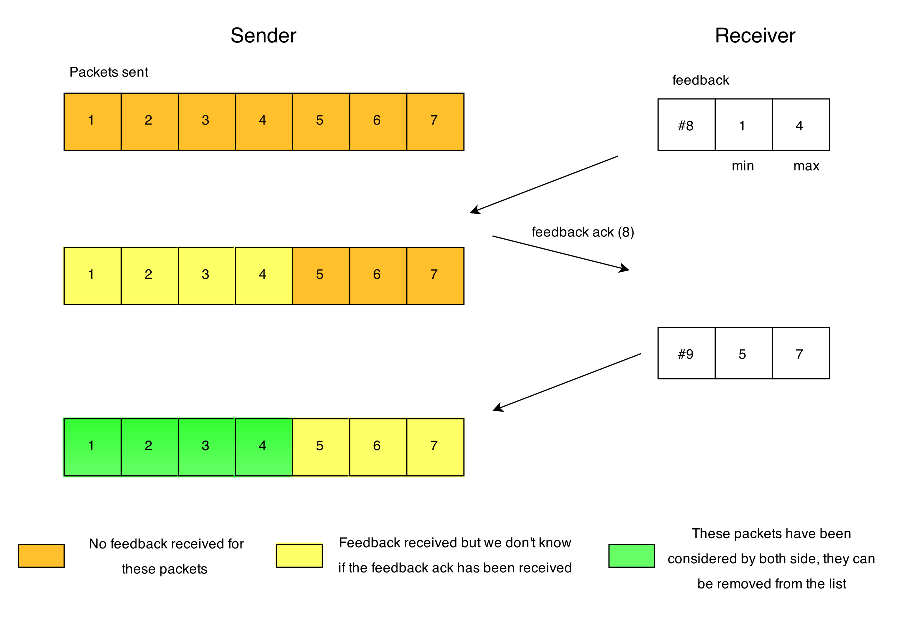
\includegraphics[width=\textwidth]{images/Feedback-implem1.eps}
\caption{How the feedback works in the sender side}
\label{fig:feedback-imp1}
\end{figure}


When a second feedback arrives, everything below the minimum sequence number reported (packets 1 to 4 in this case) can be removed from the list. The reason we can do that is because the feedback packets are cumulative. It would probably become clearer with the second example on Figure \ref{fig:feedback-imp2}. It is exactly the same scenario as before except that the \texttt{FeedbackAck} is lost. Therefore, on the next feedback, the receiver will report all the statistics from the beginning. In consequence, the sender will have to wait one more feedback to shrink the list.

\begin{figure}[!ht]
\centering
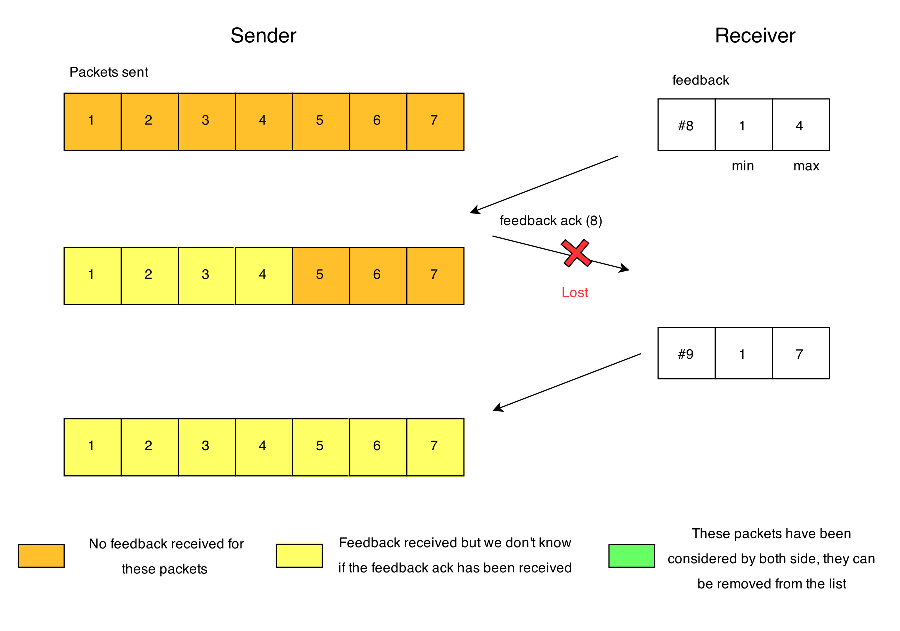
\includegraphics[width=\textwidth]{images/Feedback-implem2.eps}
\caption{How the feedback works in the sender side with losses}
\label{fig:feedback-imp2}
\end{figure}

Note that in our example the sequence numbers are sequential. It is not a requirement since in practice packets will be sent on different paths and therefore some gaps may be present between sequence numbers on a particular path. Nevertheless will still need the sequence number to be strictly increasing over time for the max-min mechanism to work well. This is guaranteed by DTLS and even if we reach the maximum sequence number allowed, the handshake must first be repeated according to \cite{RFC5246}.

The loss rate is computed every time we received a feedback on the range [min,max] carried by this feedback. This will sometimes cause to compute the loss rate on overlapping sets of packets. This is the case with the scenario presented on figure \ref{fig:feedback-imp2}: we first compute the loss rate on the packets 1 to 4 and then a second time on the packets 1 to 7. As stated in the design part, the loss rate is only an estimation of the real loss rate. However in practice, our system estimates quite accurately the real loss rate (see Section \ref{sec:perfs-loss} for more details). In addition, as recommended in Section \ref{sec:design-loss-rate}, we use an exponential average to consider new loss rates. This prevents short term statistics to impact too heavily the global loss rate of the flow.

\subsection{Receiver Side}

\subsubsection{Structure in Memory}

As for the sender statistics, every flow has to keep some information in memory to monitor the quality of the link. The C structure used is presented on Figure \ref{lst:receiver-stats}. The biggest difference with the sender is the size of the structure which is constant here. Indeed, we don't need to remember every packet received but instead only the minimum and maximum sequence number received so far.

\begin{lstlisting}[caption=Receiver structure to store statistics, label=lst:receiver-stats]
typedef struct MPDTLS_RECEIVER_STATS {
  /* information gathered since the last feedback */
  uint64_t nbr_packets_received;   /* number of packets received */
  uint     min_seq;                /* minimum sequence number */
  uint     max_seq;                /* maximum sequence number  */
  
  /* same information as before but transmitted */
  uint64_t nbr_packets_received_cache;
  uint     min_seq_cache;
  uint     max_seq_cache;
  
  uint64_t backward_delay; /* average backward delay (ms) */
  int      threshold;      /* after how many packets must we send a feedback */
  uint     last_feedback;  /* sequence number of the last feedback we sent */
} MPDTLS_RECEIVER_STATS;
\end{lstlisting}

\subsubsection{Returning feedback}

The way feedback is handled on the receiver side is way more simple than on the sender's. Indeed, we just need to support cumulative feedback. Figure \ref{fig:feedback-imp3} presents the same scenario of Figure \ref{fig:feedback-imp2} but this time on the receiver side. The feedback ack being lost, packets 1 to 4 have not been removed. Indeed, the receiver cannot make the distinction between the loss of the original feedback and the one of the feedback ack.

\begin{figure}[!ht]
\centering
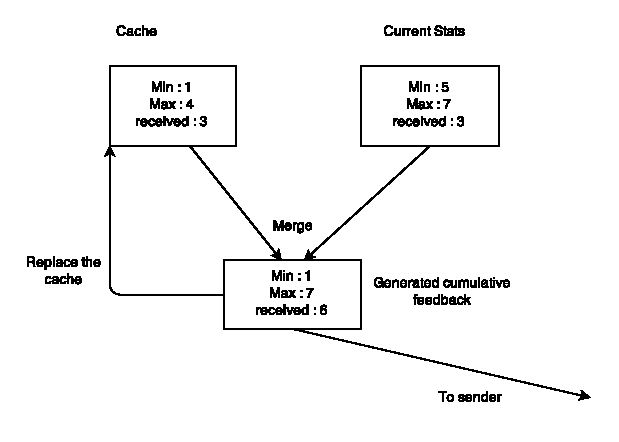
\includegraphics[width=0.7\textwidth]{images/Feedback-implem3.eps}
\caption{How the feedback is generated on the receiver side}
\label{fig:feedback-imp3}
\end{figure}

What we have called the "cache" will aggregate all previous feedback. When the threshold is reached and the receiver has to send feedback, he will first merge the current statistics with the cache to generate the cumulative feedback. The latter is sent to the sender (on the same flow) and the sequence number is remembered in the \texttt{last\_feedback} variable of Listing \ref{lst:receiver-stats}. Then the cache is replaced by this new generated feedback.


\subsubsection{Processing feedback ack}

When a feedback ack is received, the receiver must check if the sequence number corresponds to the last feedback sent. IF they match then the cache is emptied and we are in a situation similar to the one depicted on Figure \ref{fig:feedback-imp1}. The feedback ack carry the sequence number 8 which matches the latest feedback sent thus the cache containing packets 1 to 4 is emptied. Therefore the next feedback will report statistics on packets 5 to 7 only.

If the feedback ack does not contain the sequence number of the latest feedback sent we simply discard it. This kind of situations may be encountered if we have interleaving. 


\subsubsection{Computing backward delay}

The backward delay is computed thanks to regular heartbeat messages going from the sender to the receiver. These messages must transport a timestamp so we have defined a new type of heartbeat called \texttt{HEARTBEAT\_TIMESTAMP}. It allows us to differentiate this kind of message at the record layer stage and perform a different treatment than on standard \texttt{HEARTBEAT\_REQUEST}. 

To get the current time of a system, we use the \texttt{gettimeofday()} function with a \texttt{timeval} structure. It gives a microsecond precision but we actually decided to consider only the milliseconds. If there are two links we cannot differentiate at the millisecond level, we can just consider them as of equal speed (i.e. the gain will not be significant enough to treat them differently). Of course this could be adapted easily if we have a real interest for such precision and if network components become much faster.

When the receiver treats a \texttt{HEARTBEAT\_TIMESTAMP}, it computes the absolute value of the difference between his current time and the one contained in the message. This will give the backward delay with the clock desynchronization term. The receiver will add these delays and keep in memory the exponential average (variable \texttt{backward\_delay} of Listing \ref{lst:receiver-stats}). Every time it sends a feedback, it includes its estimation of the backward delay which gives the sender its forward delay.



\chapter{Evaluations and Performances}\label{chap:perfs}

\section{Test application}\label{sec:vpnapp}

MPDTLS is implemented inside a library, we thus need a suitable application to use this library. We tried to find out which application could be a good candidate for our tests. First, we needed an application which uses DTLS for most of its communications and is open source. It was surprisingly hard to find but we still managed to find one : Campagnol\cite{campagnol}. Campagnol is a decentralized VPN solution which is using DTLS to communicate between the peers. Unfortunately, for a set of reasons exposed in Appendix \ref{app:campagnol}, we were unable to integrate correctly our modified library within the application. 

So, we took the decision to build our own VPN application \cite{wolfssl-vpn} and reuse part of Campagnol's code. A VPN application is indeed perfectly suitable for all the experiences we could imagine : potentially any application can use a VPN tunnel without even noticing it. Every packet is encapsulated inside a DTLS packet transmitted securely between the two MPDTLS hosts (see Figure \ref{fig:vpn}).

\begin{figure}[!ht]
\centering
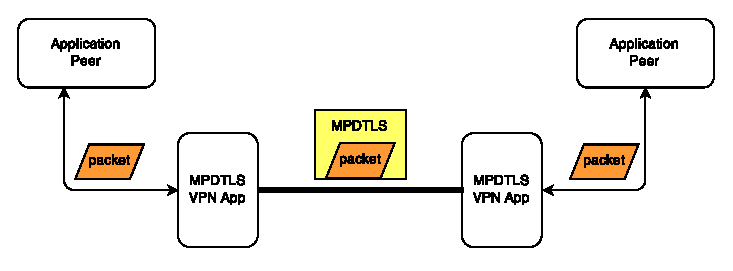
\includegraphics{images/vpn.eps}
\caption{A simple VPN application using MPDTLS}
\label{fig:vpn}
\end{figure}

The behavior of one of this MPDTLS VPN App is shown on Figure \ref{fig:vpn-io}. A TUN interface is created with a specified address and netmask. Every packet going to an address falling in this netmask will be sent by the kernel to this interface. What we need then is to monitor this interface, read the packets that have arrived and sent them through the tunnel. This is the job of the first thread (in red on the Figure). We also need to capture packets coming from the network and write them in the TUN interface. This is handled by a second thread represented in green on the Figure. Finally, a last thread (in blue) is listening the standard input for potential commands. This is the channel we use to communicate with the application to add or remove new interfaces for instance. We can ask for debug information or even change the scheduler policy on the fly.

\begin{figure}[!ht]
\centering
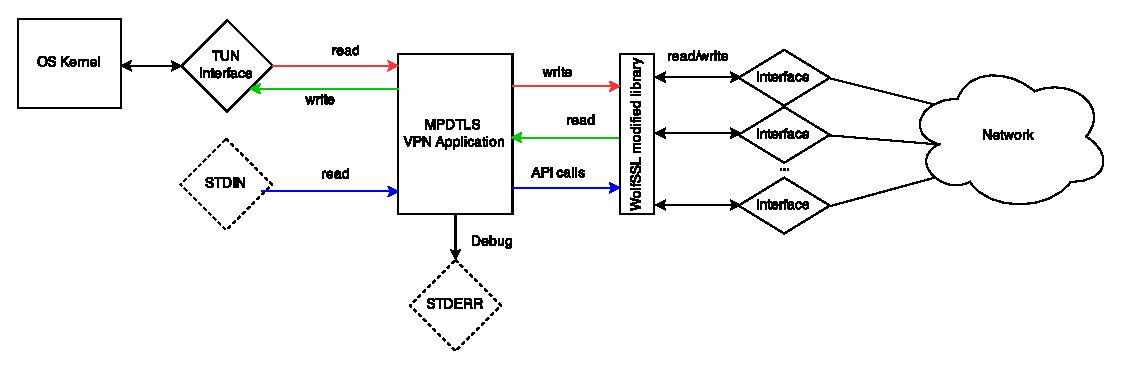
\includegraphics[width=\textwidth]{images/tunneling-IO.eps}
\caption[I/O interactions for one host of our application]{I/O interactions for one host of our application. Each thread is represented with one color.} 
\label{fig:vpn-io}
\end{figure}

One of the most useful information we can ask for are the statistics for a particular flow. Just by looking at this output, we can most of the time identify a problem without even looking at the Wireshark trace. An example of such an output is shown on Listing \ref{lst:stats}. We can easily see the part of traffic the flow is actually supporting, the estimated delays and other information. The separator | is used in the packets sent list to differentiate the ones that are in the waiting state and the others (see Section \ref{sec:impl-stats} for more details about this waiting state).

\begin{lstlisting}[language=bash,caption=An output of the statistics for a particular flow,label=lst:stats]
---- Stats Flow N 0 ---- 
IP src : 11.0.0.1 
IP dst : 11.2.0.1 
Support 41 % of the connection
----- Receiver Stats ----- 
Packets received : 44 
Min_Seq received : 76 
Max_Seq received : 172 
Backward delay : 10 ms
----- Receiver Cache ----- 
Packets received : 0 
Min_Seq received : 2147483647 
Max_Seq received : 0 
----- Sender Stats ----- 
Packets sent : [ 8487 8489 8492 ... 8633 8634 8636 | 8640 8642 ... 8706 8707] 
Forward delay : 10 ms
Loss Rate : 0.000000 
---------------------------

\end{lstlisting}

\section{Different scheduler policies}\label{sec:perf-sched}

We present here the different scheduler strategies we have implemented and how the fractional distribution is computed in each case. At the end each of them has pros and cons, the good choice is strongly related with what the underlying application expect to do. It may even be needed that an application has to build its own scheduler and that is perfectly fine with our design since we have a dedicated callback.

\subsection{Round Robin}

The round robin is the simplest strategy consisting in giving the same amount of traffic to each of the available links. This does not use any of the information gathered with the feedback. However it may be a good choice if we know in advance that the different links are sharing common properties (e.g. in a datacenter).

The fractional distribution is really easy to compute as every link will get the same fraction of traffic.

\begin{equation*}
f_i = \frac{1}{n}
\end{equation*}

where $f_i$ is the portion of traffic given to flow $i$ and $n$ is the total number of flows.

\subsection{Optimize Latency}

For this strategy, we want to give more weight to links where the forward delay is lower. We have to keep in mind that in every delay $d_i$, we have the clock desynchronization term (see Section \ref{sec:forward-delay}). In order to get rid of this term, we must consider the difference with another delay. We choose to take the difference with the maximum delay as by definition the greater the difference, the smaller the delay. Equation \ref{eq:latency} gives the complete expression.  

\begin{equation}
f_i = \frac{max_d - d_i + \alpha}{\sum_j (max_d - d_j) + n*\alpha }\quad \text{where } \quad max_d = max_i(d_i) 
\label{eq:latency}
\end{equation}

Without the $\alpha$ term, the flow with the maximum delay will never be used. Indeed if you have two flows with forward delays of 10ms and 20ms and $\alpha=0$, then $100\%$ of the traffic will be supported by the first flow. Although this may be a desired choice, it is always preferable to let a minimal part of the traffic on every link just to monitor the characteristics and keep receiving feedback and heartbeat messages. After some tests, we think the value of $\alpha$ must be chosen between 5\% and 10\% of $max_d$\footnote{Of course, $max_d$ must not be null. If it is the case, then a constant value must be chosen like 1ms and the equation will actually give the same result as a round robin.} to give the best results. 

\subsection{Optimize losses}

Another strategy we could think of is to favor the most reliable links. We thus give more priority to a link with a smallest loss rate. The principle is almost the same as for the latency, we will consider the difference with the biggest loss rate observed. We may be tempted to use directly the loss rate reported in the statistics. However if the link experiences a lot of losses, we may not be aware because all the feedback packets have been dropped. Therefore we compute what we call the "real" loss rate which takes also in consideration the number of packets sent and not yet acknowledged. Equation \ref{eq:lr} gives the formula used and $feedback_{thr}$ is the number of packets after which we send a feedback. We consider two times this amount to give a penalty to the link because after one feedback, packets are in waiting state and need another feedback to be completely forgotten. The penalty $pen$ is computed as two times the probability of loosing one feedback. The factor $2$ here will probably need some tuning but the idea is to boost the penalty as the chance to loose just the feedback packet and none application data is rather small. 



\begin{align}
LR_i &= stats_{LR} + \left \lfloor{\frac{pckts_{sent}}{2 * feedback_{thr}}} \right \rfloor  * pen & \text{where } \quad pen = \frac{1}{feedback_{thr}} * 2 \label{eq:lr} \\
f_i &= \frac{max_{LR} - LR_i + \beta}{\sum_j (max_{LR} - LR_j) + n*\beta } & \text{where } \quad max_{LR} = max_i(LR_i) 
\label{eq:losses}
\end{align}

Equation \ref{eq:losses} is really similar to Equation \ref{eq:latency} and we also need a constant term $\beta$ for the same reasons. After some tests, we arrive at the conclusion that a suitable value for $\beta$ is around $0.01$ loss rate in most of the situations.

\section{Multipath simulations}

We have designed an environment to evaluate our system under different conditions. All the following measures take place inside a mininet laboratory \cite{mininet} to easily set up the topology we want and create multiple interfaces. Also, we used a kind of framework for mininet called Minitopo to easily configure the topology and create automated tests just with configuration files instead of scripts. To generate network traffic, we used the D-ITG (Distributed Internet Traffic Generator)\cite{ditg} tool.

\subsection{Topology}

The topology used for the following evaluations is the one presented on Figure \ref{fig:topo-phys}. We have four interfaces on the client side that are linked with a network switch and one link between the switch and the server. Note that the latter is not constrained, we will only change the characteristics of the first 3 paths shown on the Figure. The path 4 is reserved for the signaling of D-ITG thus avoiding any interference with our measures.


\begin{figure}[!ht]
\centering
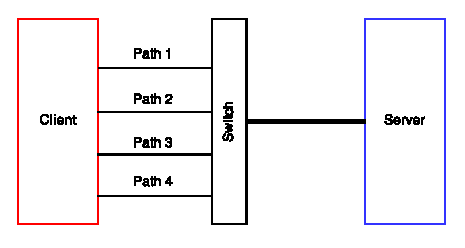
\includegraphics[width=0.8\textwidth]{images/perf-topo-phys.eps}
\caption{Physical topology inside mininet}
\label{fig:topo-phys}
\end{figure}

The corresponding logical topology is depicted on Figure \ref{fig:topo-log}. We are using 3 flows concurrently between the client and the server. The ITG application is sending traffic to one unique TUN interface and the traffic goes through our tunnel to reach the ITG receiver.

\begin{figure}[!ht]
\centering
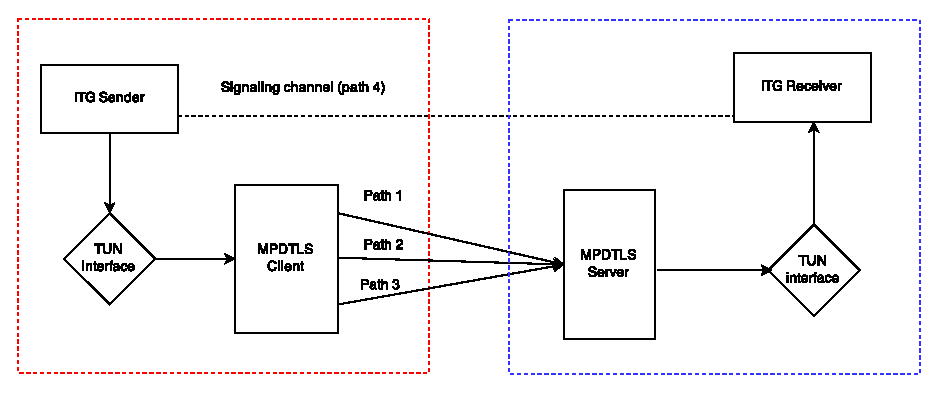
\includegraphics[width=\textwidth]{images/perf-topo-logic.eps}
\caption{Logical topology used for measurements}
\label{fig:topo-log}
\end{figure}

\subsection{Traffic balancing}

The first thing to evaluate is if we really take advantage of multiple interfaces and how we balance the traffic between them. We will run some experiments to determine in which conditions each scheduler performs well and how they compute the distribution of traffic in various environments.

\subsubsection{With dynamic bandwidth}

In this experiment, we have tested the two schedulers that are taking the context into consideration : \texttt{Optimize Latency} and \texttt{Optimize Loss}. The configuration used is the following (the path numbers are referring to Figure \ref{fig:topo-log}) :


\begin{table}[!h]
\centering
\begin{tabular}{|c|c|c|c|}
\hline
Path n\degree & bandwidth & loss rate & delay  \\ \hline
1 &  1 Mbps & 0 & 10ms \\ \hline
2 & variable & 0 & 20ms \\ \hline
3 & not used & - & - \\ \hline
\end{tabular}
\end{table}

The goal is to modulate the bandwidth of B and see how its usage rate is impacted. We have generated constant traffic with D-ITG \cite{ditg} using both UDP and TCP. All these results are reported in Figure \ref{fig:dynbw}. The measures have been obtained during sessions of 60 seconds and every experiment has been repeated 11 times to evaluate the mean. The 95\% confidence interval of the mean is presented in white and has been computed with a Student T distribution.


\begin{figure}[!h]
\centering
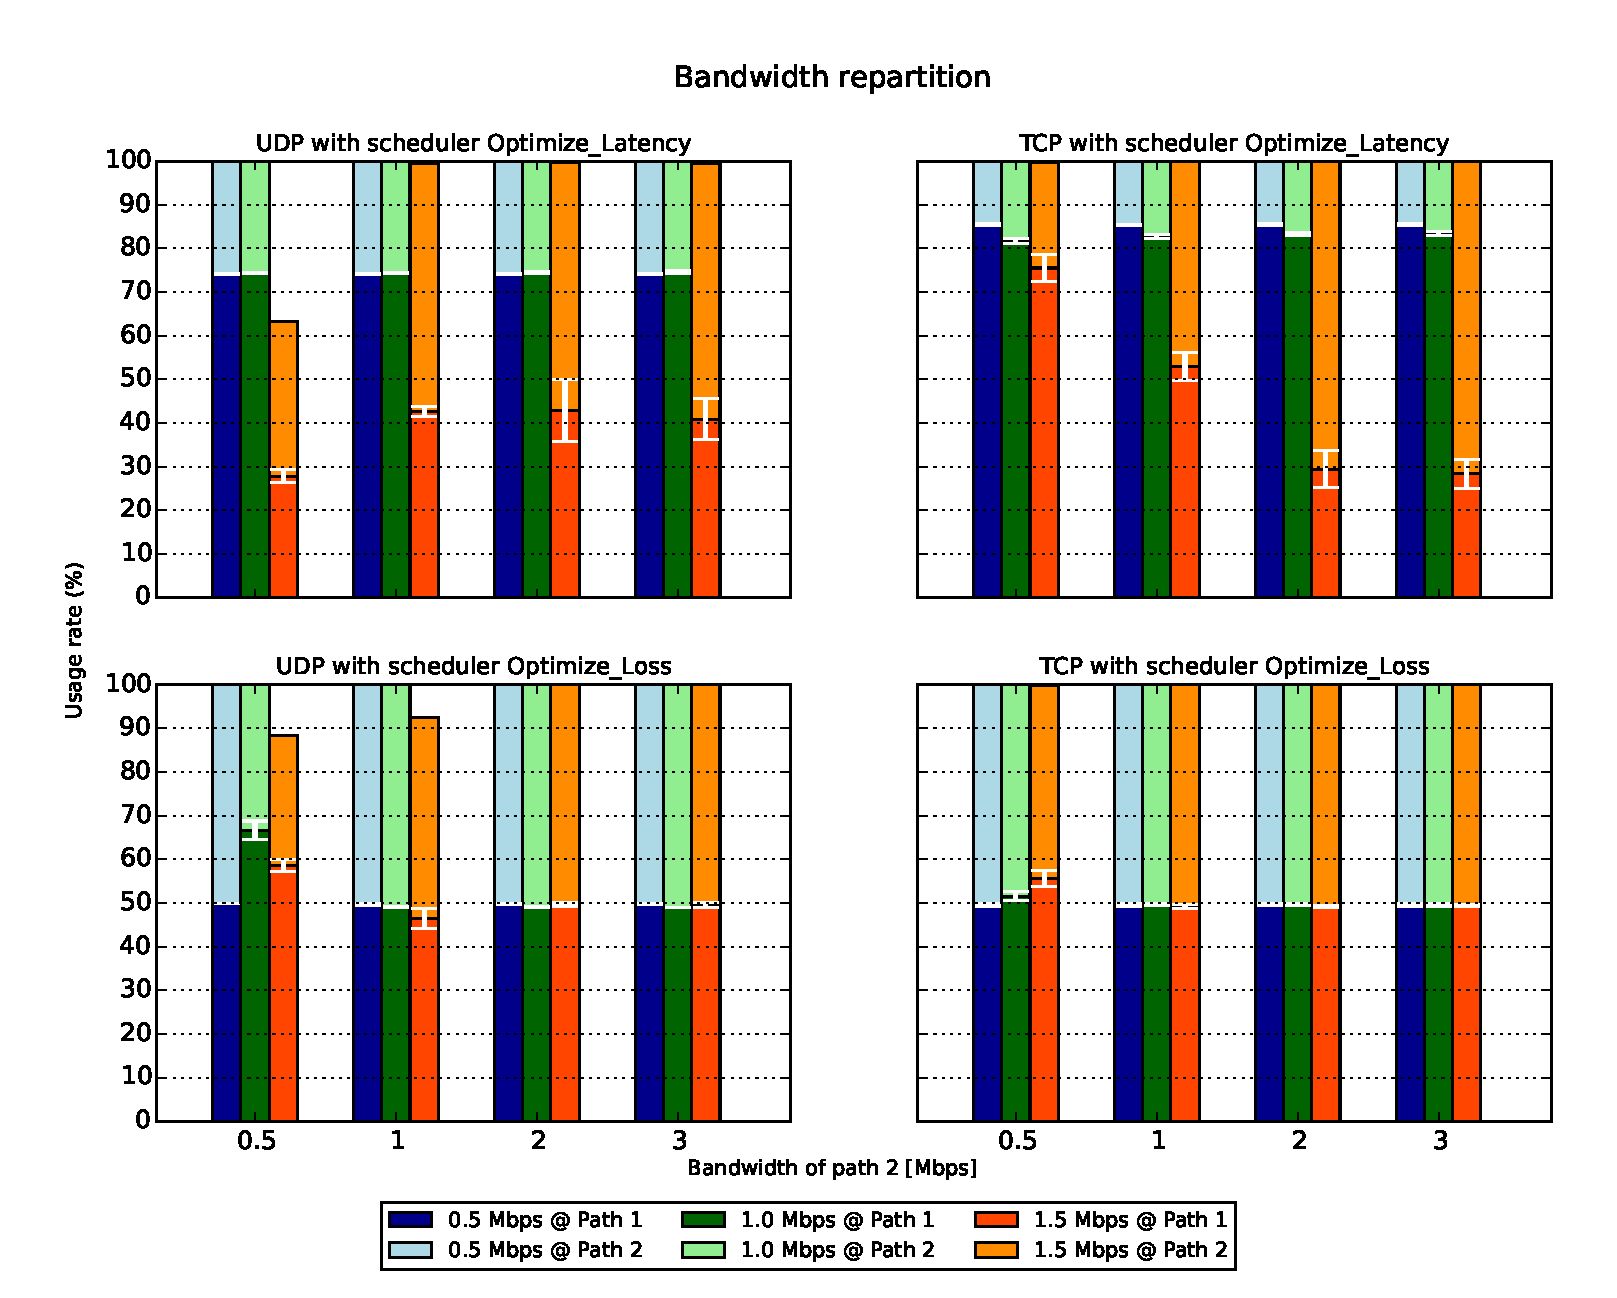
\includegraphics[width=\textwidth]{images/xp/graph1.eps}
\caption{Usage repartition with bandwidth variation}
\label{fig:dynbw}
\end{figure}


For every bandwidth value of path 2, we have 3 bars that represent the total amount of traffic we are trying to send through the tunnel. Each bar is separated in two parts that are showing the percentage of traffic passing through each path. The losses are easily identifiable because they occur every time the sum of the usage rates does not reach 100\%. Of course at the beginning we have congestion because if path 2 can support only $0.5Mbps$ then $bw(p1) + bw(p2) = 1.5Mbps$ and in the last case we are trying to send traffic at 1.5Mbps. So, it is supposed to use 100\% of the tunnel capacity which is impossible in practice due to our random scheduler. Moreover, this computation is not even taking into account the overhead introduced with the encapsulation inside DTLS. Indeed, we are sending packets of size 825 bytes inside the TUN interface and the resulting size of the DTLS \texttt{ApplicationData} packet is 905 bytes; so an overhead of almost 10\%.

First, it is interesting to confirm that the \texttt{Optimize loss} scheduler performs better if we are dealing with congested links and especially with UDP. Note that TCP doesn't experience losses the same way as UDP because it will reduce its emission rate internally with the congestion window mechanism. So even if we impose a certain amount of traffic, the real bandwidth will be lower with TCP in case of congestion.

Secondly, we observe a strange phenomenon if we look at the graph "UDP with scheduler Optimize Latency" : when we increase the total bandwidth to 1.5Mbps (orange), it does not optimize latency at all. Indeed, it gives only 28\% of the traffic to the faster link. We have tracked down the problem and it is apparently coming from a bad perception of the forward delay. At the beginning, it will use extensively path 1 as expected but will rapidly reach congestion as the capacity of path 1 is 1Mbps. The heartbeat messages that are used to evaluate the forward delay are themselves postponed by a few milliseconds due to this congestion and it is enough for the scheduler to estimate the delay is better on path 2. Even if later the forward delay is correctly estimated, we go back in the same cycle.  It is not the case with TCP at least at the beginning because TCP reduce the bandwidth to fit into the tunnel and therefore no congestion is observed.

\subsubsection{With dynamic loss rate}\label{sec:perfs-loss}

This time, we want to see how the schedulers will react if we progressively increase the loss rate of one of the path. The configuration is the following :

\begin{table}[!h]
\centering
\begin{tabular}{|c|c|c|c|}
\hline
Path n\degree & bandwidth & loss rate & delay  \\ \hline
1 &  1 Mbps & 0 & 10ms \\ \hline
2 & 3 Mbps & variable & 10ms \\ \hline
3 & not used & - & - \\ \hline
\end{tabular}
\end{table}

Again we are using 2 paths only and they have the same latency but different bandwidth. We increase the loss rate of path 2 from 0\% to 3\% gradually. The results we have obtained are presented on Figure \ref{fig:dynloss}.


\begin{figure}[!h]
\centering
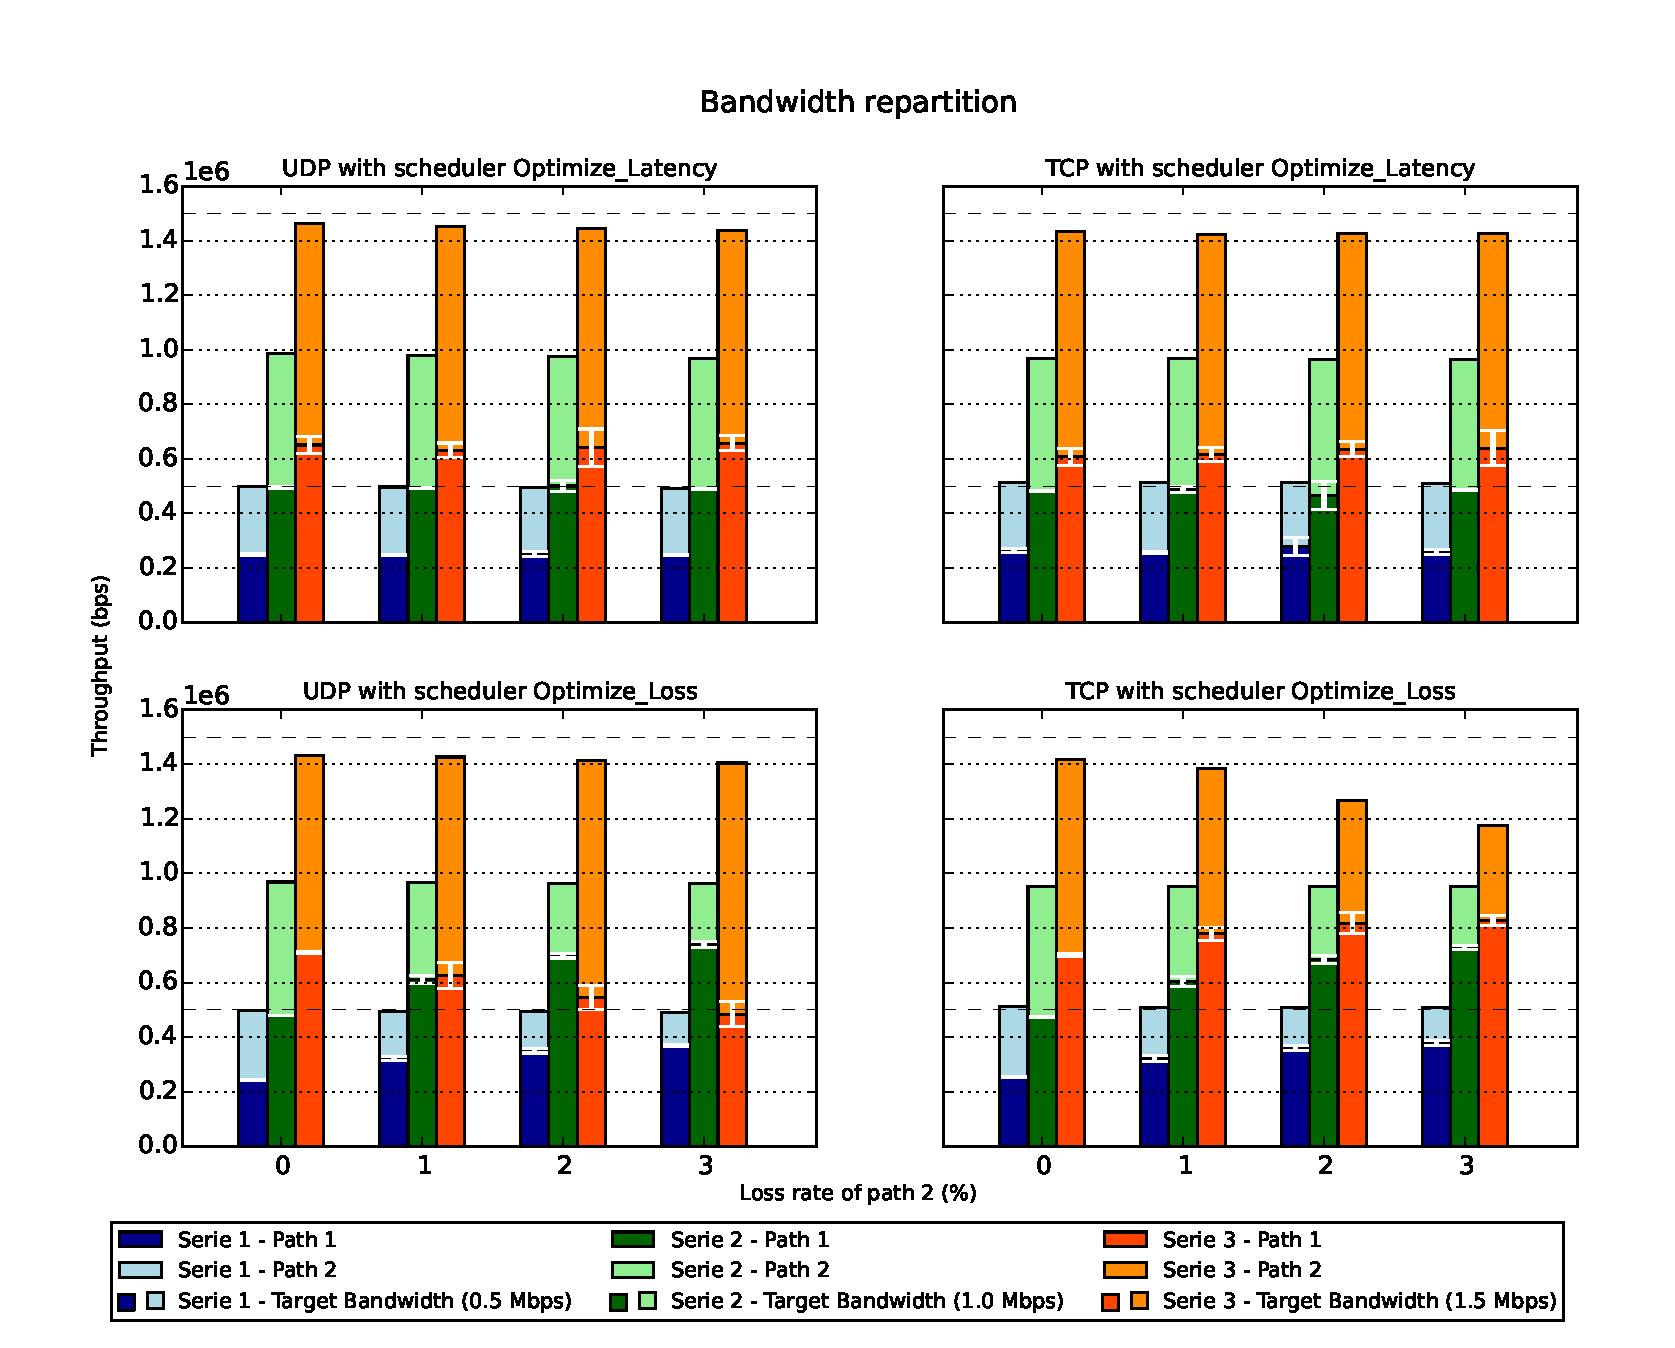
\includegraphics[width=\textwidth]{images/xp/graph2.eps}
\caption{Usage repartition with loss rate variation}
\label{fig:dynloss}
\end{figure}

A first thing to point out is the fact the scheduler \texttt{Optimize Latency} is not really impacted by the loss rate as we can expect. The proportion is always around 50\% for both TCP and UDP as the two links have the same delay. The little exception to this rule is noticed for the third bar (traffic at 1.5Mbps) probably because we reach the congestion limit on path 1. Therefore, the heartbeat messages are either delayed or dropped and the forward delay is overestimated.

On the other hand, the scheduler \texttt{Optimize loss} will progressively give more weight to the first path as it is loss free. We notice that UDP and TCP give different results concerning the latest bar which corresponds to the 1.5 Mbps transfer speed. Again, this can be explained by the congestion on path 1. UDP will keep sending packets even if they are dropped, therefore the scheduler will see important losses on path 1. The loss rate caused by congestion will overcome the one of path 2 and the scheduler will thus choose the best option among the two. However, for TCP, the congestion control mechanism will reduce the sending rate to avoid path 1 of being congested. In such conditions, path 1 remains the best option and thus is given more weight by the scheduler.


\subsection{Resiliency to interface removal}

The objective of the multipath is not only to do traffic balancing on exiting paths but also to modify dynamically the distribution of traffic if one interface becomes unavailable. For this experiment, we are using the topology of Figure \ref{fig:topo-log} with the following configuration : 

\begin{table}[!ht]
\centering
\begin{tabular}{|c|c|c|c|}
\hline
Path n\degree & bandwidth & loss rate & delay  \\ \hline
1 & 5 Mbps & 0 & 10ms \\ \hline
2 & 5 Mbps & 0 & 20ms \\ \hline
3 & 5 Mbps & 0 & 40ms \\ \hline
\end{tabular}
\end{table}

We will generate constant UDP traffic at 3 Mbps and observe the behavior of the implementation if the interface of path 1 is suddenly lost at $t=19s$. The bandwidth repartition is shown on Figure \ref{fig:xp-lossint-bw} and the scheduler used is \texttt{optimize loss}.


\begin{figure}[!ht]
\centering
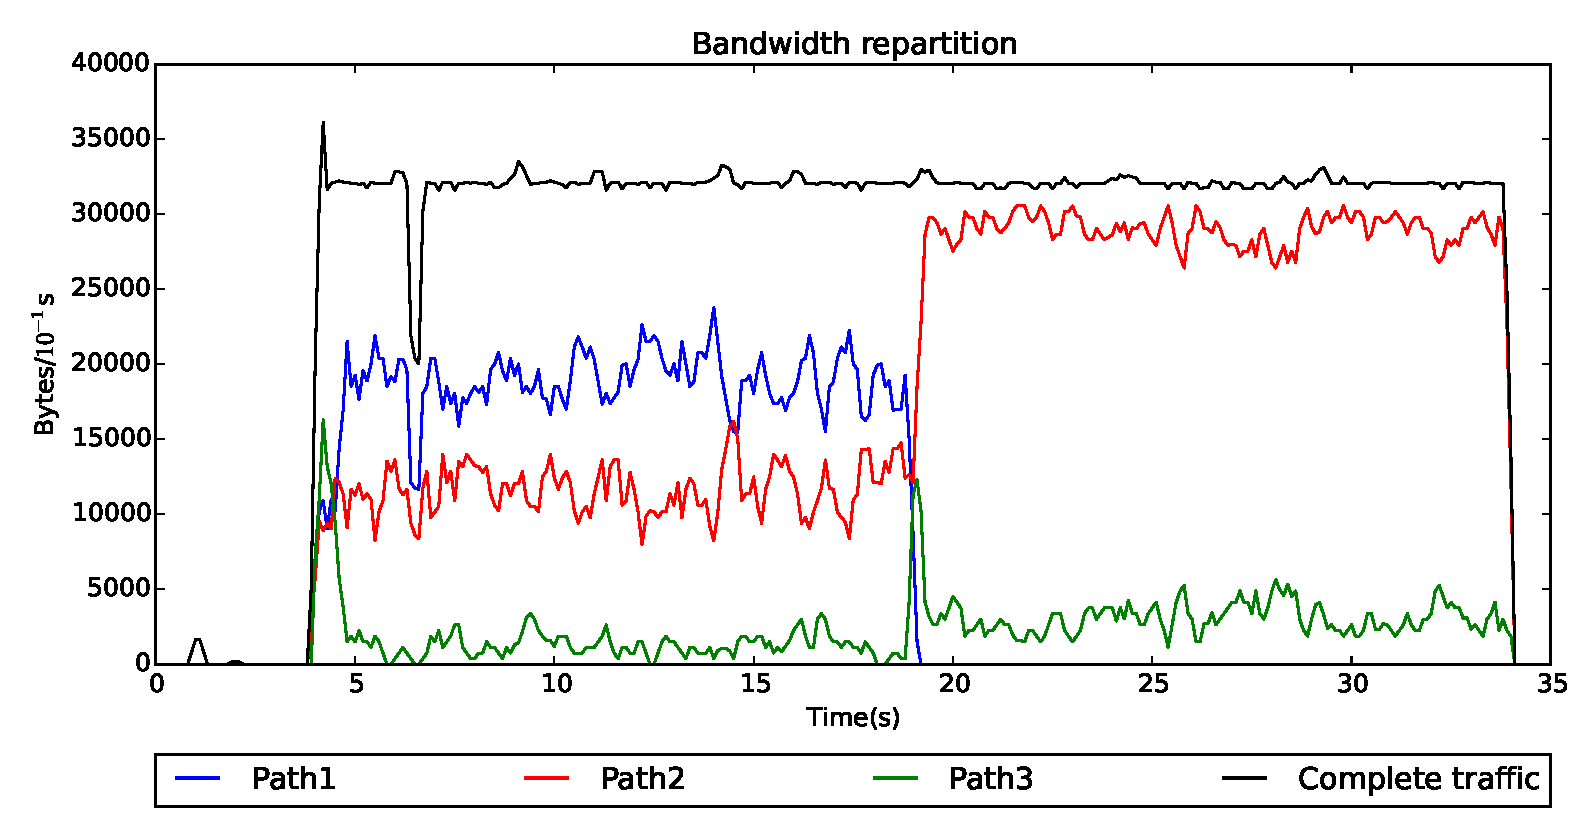
\includegraphics[width=\textwidth]{images/xp/intlost_bw.eps}
\caption{Reaction to interface removal}
\label{fig:xp-lossint-bw}
\end{figure}

Note that the path 1 was used for the handshake and we prove here that even if we remove our "primary" interface, the connection keeps going fluently. In the very first moments (at 4s), we see that the distribution is more or less equal between the flows. This setup time is needed to obtain some information about the forward delay. Heartbeat messages and feedback packets have to be exchanged between the two hosts. After 5 seconds, we see that the distribution is shaped with what we can expect from Equation \ref{eq:latency}: path 1 has almost $2/3$ of the traffic because he has the best delay, path 2 is still used because the difference of delays with path 1 is acceptable and then some traffic is given to path 3 to monitor the link.

When we loose the interface of path 1, the distribution is recomputed and most of the traffic will be re-routed to flow 2. Of course we are far from the congestion because each link has a bandwidth of 5 Mbps but the objective here was to see how the distribution is moving without other constraints. In this context, the scheduler is doing well by optimizing the overall latency as we can see in Figure \ref{fig:xp-lossint-delay}. After the loss of the fastest path, the overall delay is increased and is little above the  20ms threshold which is the delay of the new fastest link. We can also observe two peaks: the first one is due to the setup time and the second one is a temporary increase of path 3 usage to compensate the loss.



\begin{figure}[!t]
\centering
\begin{minipage}{0.4\linewidth}
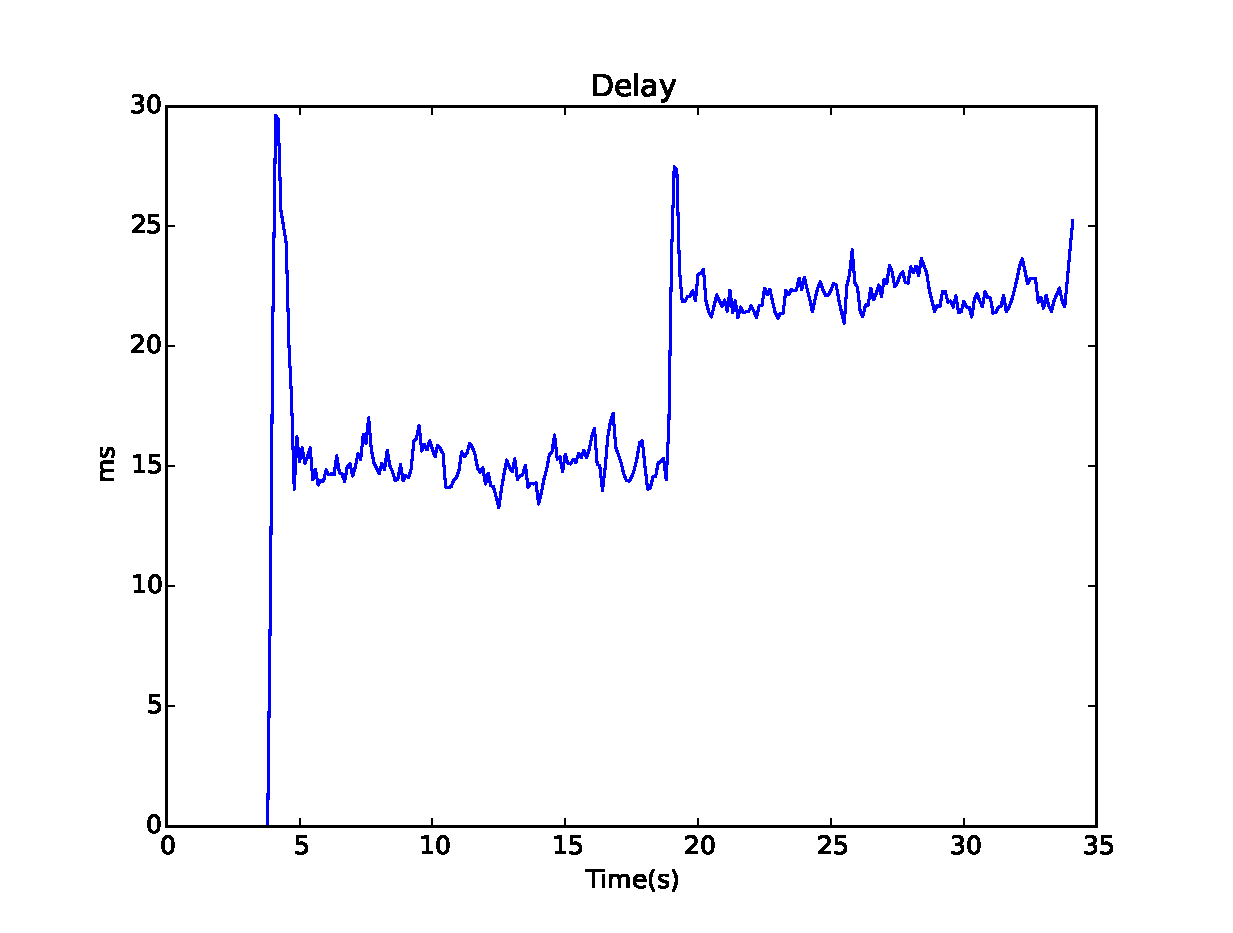
\includegraphics[width=\textwidth]{images/xp/intlost_delay.eps}
\caption{Overall delay}
\label{fig:xp-lossint-delay}
\end{minipage}
\begin{minipage}{0.59\linewidth}
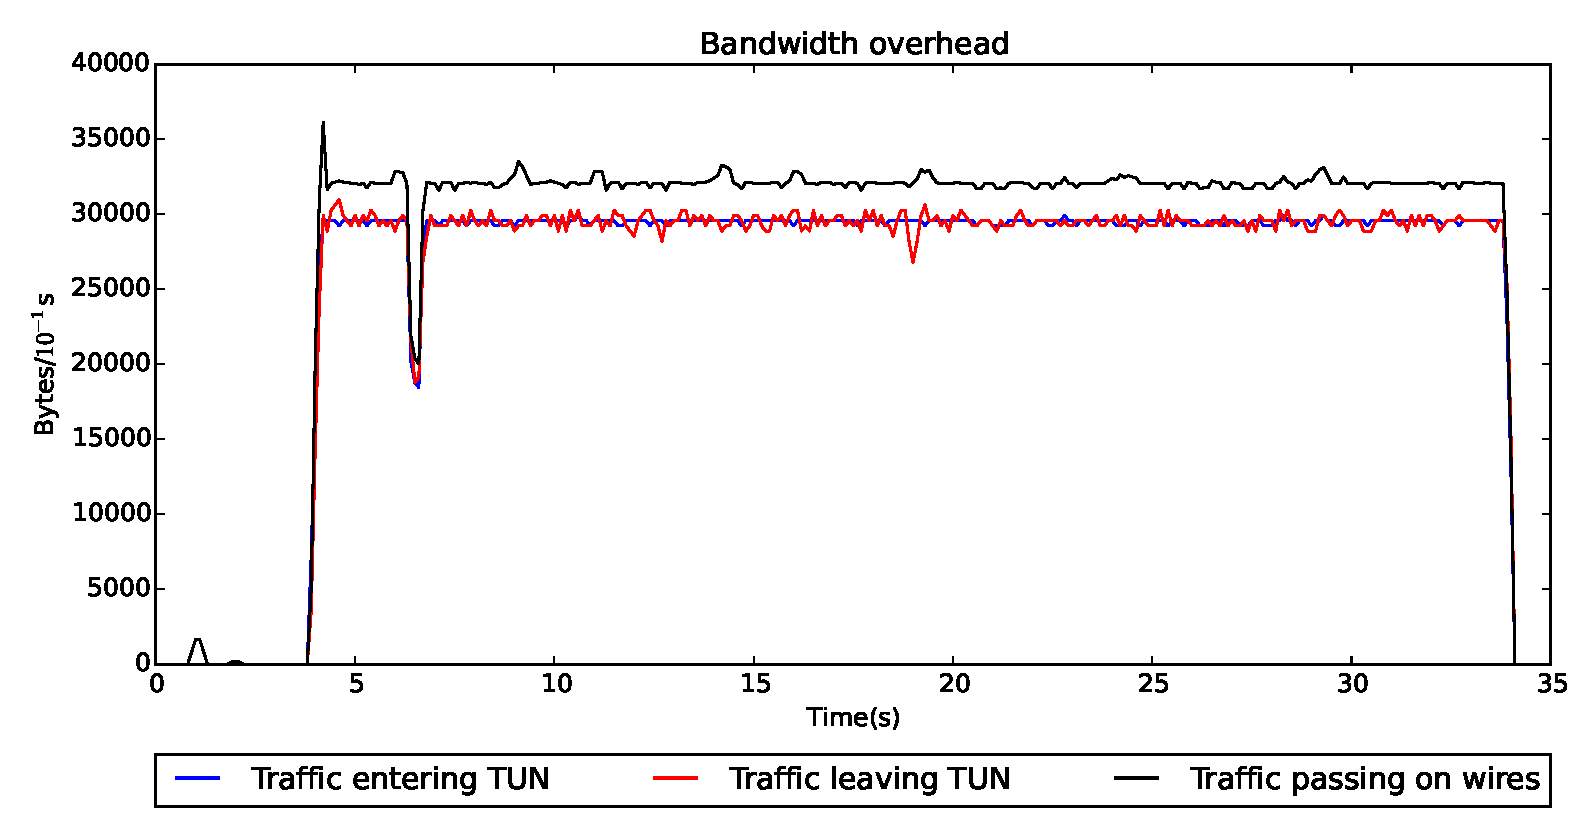
\includegraphics[width=\textwidth]{images/xp/intlost_tun.eps}
\caption{Application perception of traffic}
\label{fig:xp-lossint-tun}
\end{minipage}
\end{figure}

From the application point of view, the impact of such loss is shown in Figure \ref{fig:xp-lossint-tun}. We see in blue the traffic entering the tunnel which is constant here because we have parametrized D-ITG to do so, in red we see the traffic leaving the tunnel and in black we have the traffic generated by the tunnel. The difference between the blue and the black curve is the overhead caused by the encapsulation of D-ITG packets inside DTLS ones. Around the $19^{th}$ second, we notice a really small drop on the red curve, exactly when the interface was lost. This is the only thing the application will perceive from the loss of one interface. This is a huge improvement in comparison with a normal DTLS connection, which would ended the communication in case of such interface loss.

\begin{figure}[!ht]
\centering
\end{figure}

\subsection{Smooth add of a new interface}

In this section, we explore the reverse scenario: when one interface becomes available. At the beginning only path 1 and path 2 are available and at time $t=30s$ we add path 3. The configuration used is the following :

\begin{table}[!ht]
\centering
\begin{tabular}{|c|c|c|c|}
\hline
Path n\degree & bandwidth & loss rate & delay  \\ \hline
1 & 5 Mbps & 0 & 30ms \\ \hline
2 & 5 Mbps & 0 & 40ms \\ \hline
3 & 5 Mbps & 0 & 10ms \\ \hline
\end{tabular}
\end{table}

As we can see path 3 is faster and we expect it will take the lead over the two other ones. This is verified with our experiment as we can see on Figure \ref{fig:xp-addint-bw}. A significant portion of traffic is redirected through the new flow. At the beginning path 1 was the faster link so it was given the biggest part. But after the addition of the new interface, a re-computation is made according to equation \ref{eq:latency} and path 1 is less used.


\begin{figure}[!ht]
\centering
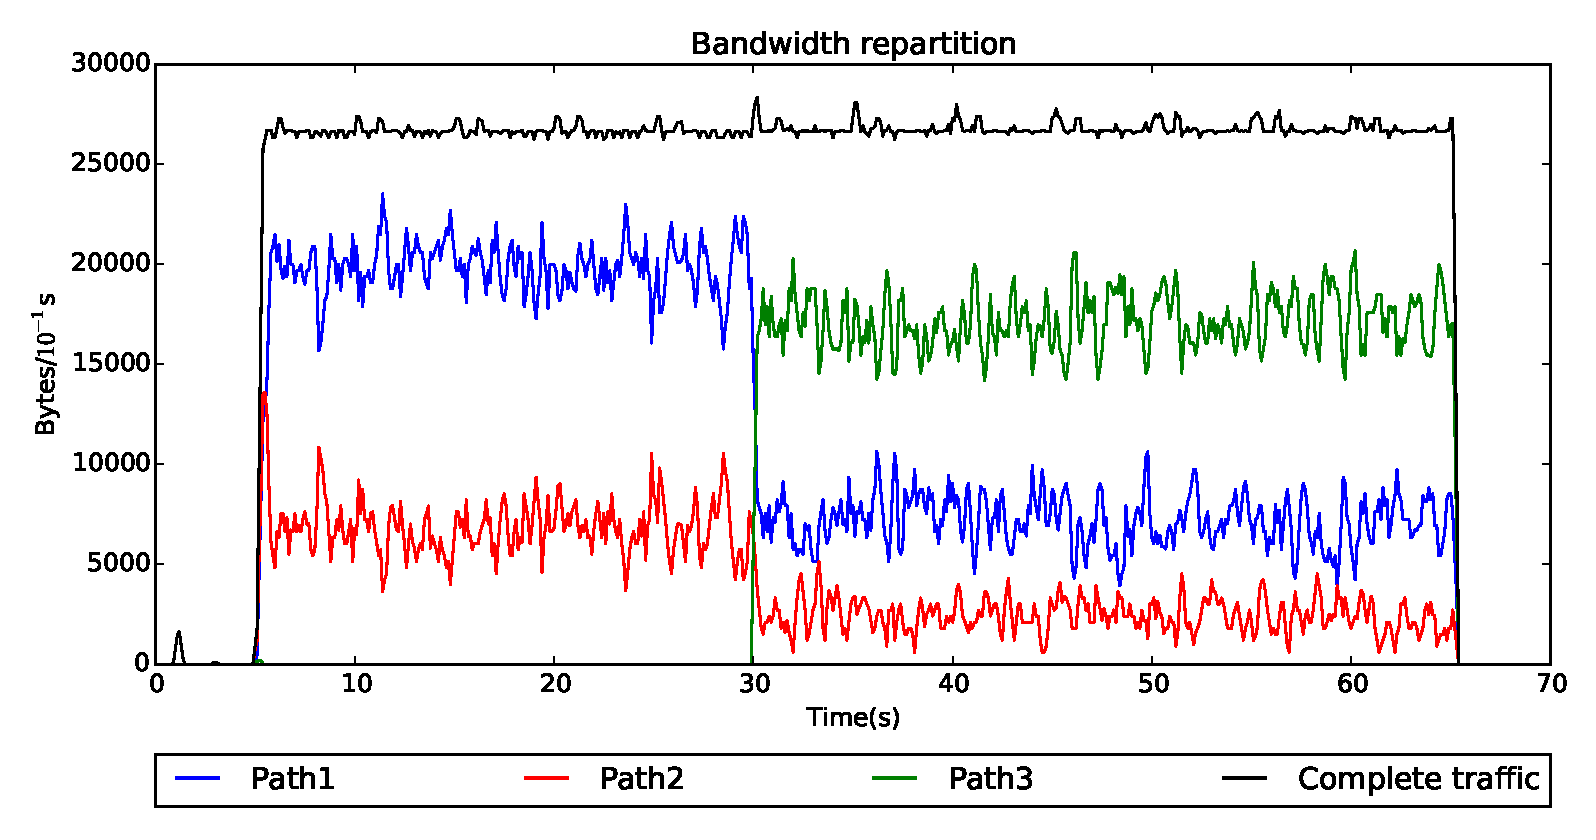
\includegraphics[width=\textwidth]{images/xp/addint_bw.eps}
\caption{Reaction to new interface addition}
\label{fig:xp-addint-bw}
\end{figure}

The overall delay is kept reasonably small according to Figure \ref{fig:xp-addint-delay} but we could probably optimize even more. That would imply putting more weight to path 1 and thus offload the two other flows. However this is a choice we have made to keep using all the paths while still trying to give more traffic to the faster link. It will allow for quicker recovery if the best interface is lost.

\begin{figure}[!ht]
\centering
\begin{minipage}{0.4\linewidth}
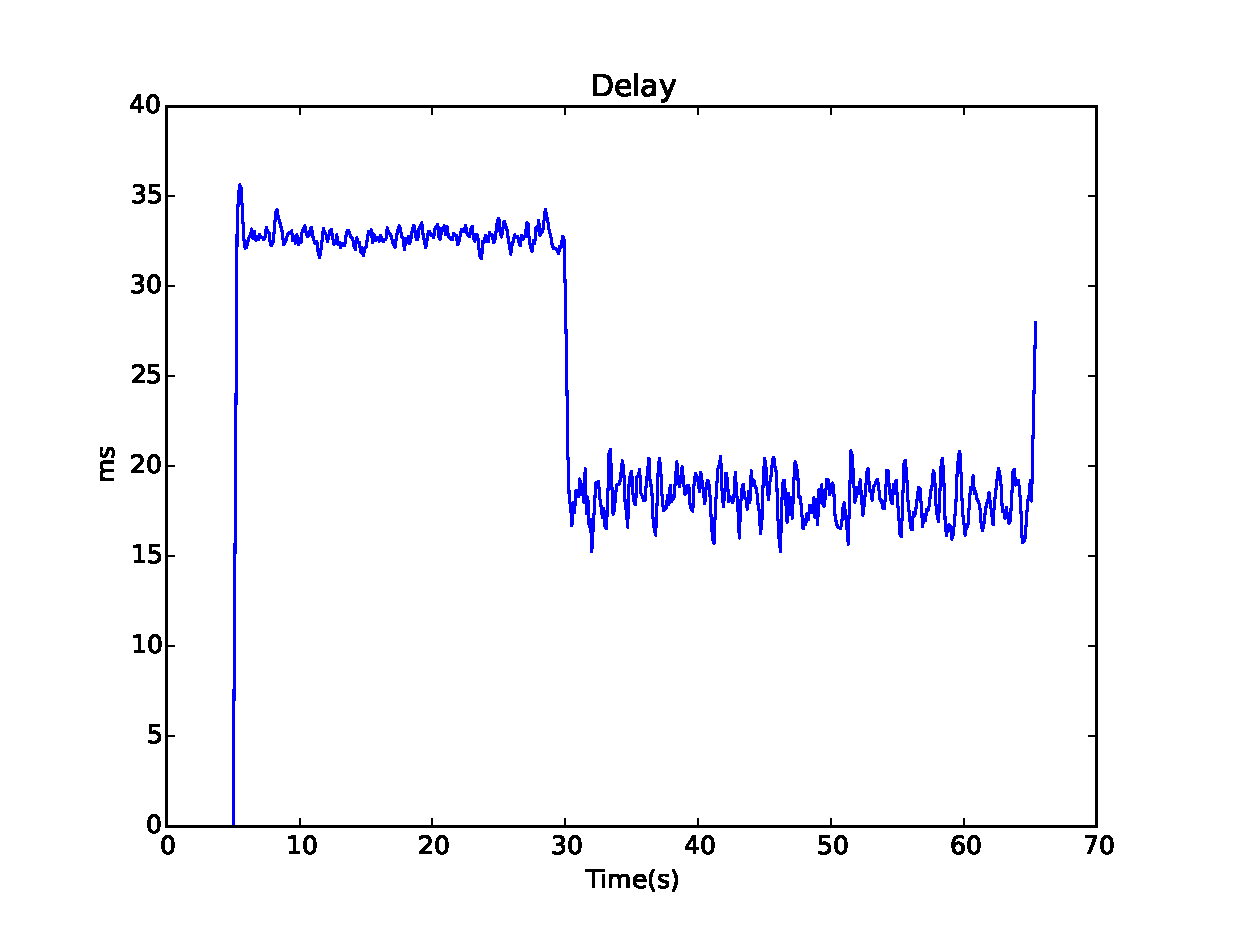
\includegraphics[width=\textwidth]{images/xp/addint_delay.eps}
\caption{Overall delay}
\label{fig:xp-addint-delay}
\end{minipage}
\begin{minipage}{0.59\linewidth}
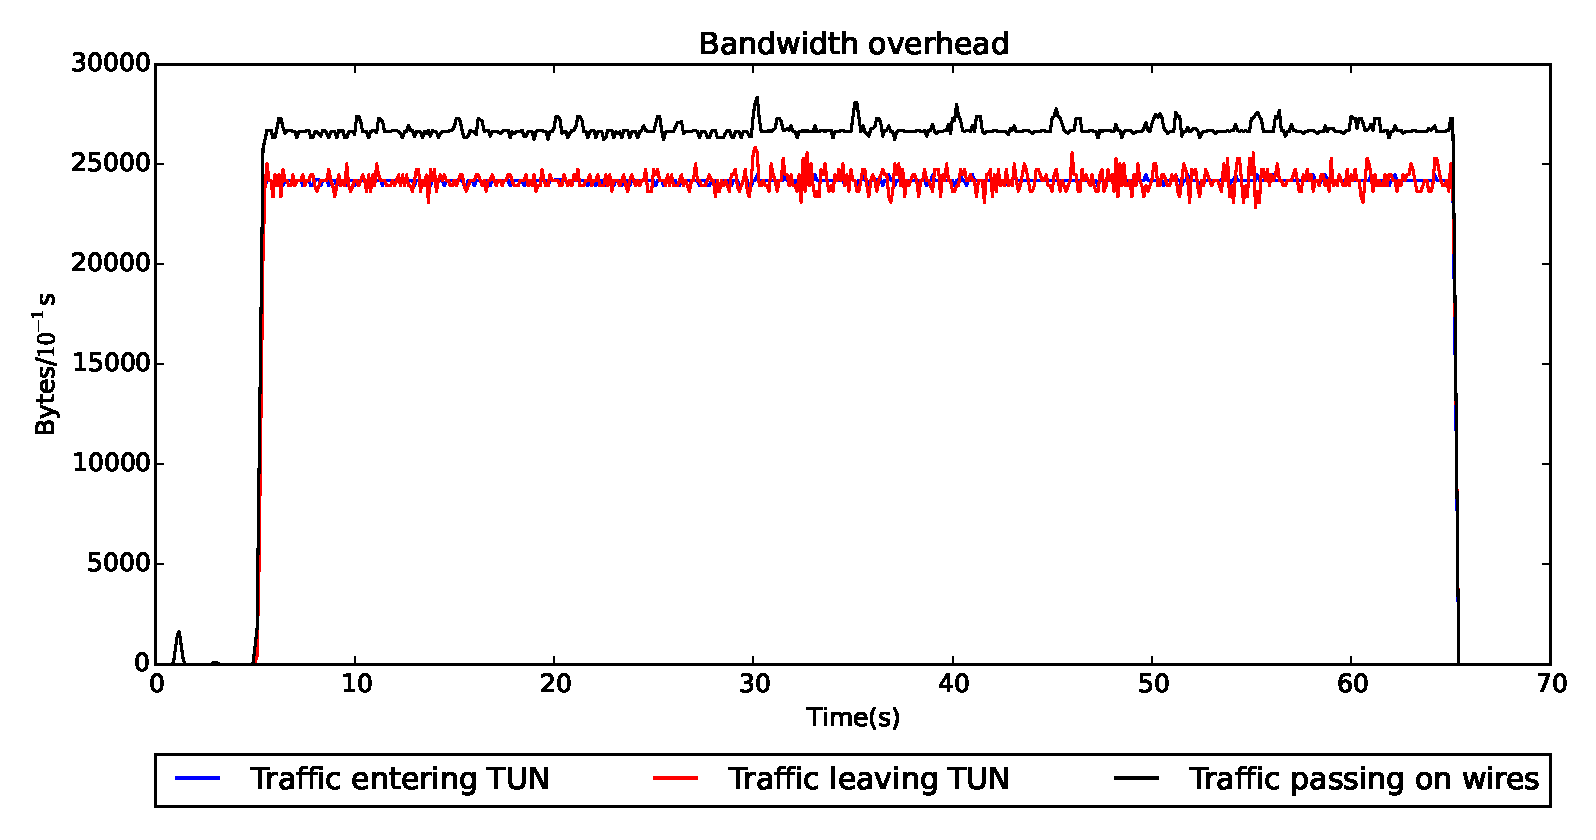
\includegraphics[width=\textwidth]{images/xp/addint_tun.eps}
\caption{Application perception of traffic}
\label{fig:xp-addint-tun}
\end{minipage}
\end{figure}

If we look at the traffic perceived by the application on Figure \ref{fig:xp-addint-tun}, we notice no real perturbation around $30s$. Although the traffic is a bit noisy after this time, this is explained by the fact we have 3 different paths with 3 different delays and therefore packets cannot arrive at a constant rate.

\section{Conclusion}

In this chapter, we have presented the VPN application we have designed to evaluate our MPDTLS implementation. To dispatch efficiently the packets between the available flows, 3 schedulers have been created : Round Robin, Optimize Loss and Optimize Latency. We have concentrated our evaluation on the last two since the round robin doesn't consider any contextual information. 

After various experiments, we have shown that the scheduler \texttt{Optimize Latency} behaves better when there is no congestion. Otherwise, it will try to push a great amount of traffic on the faster link and quickly triggers congestion. However, we have discovered that the counter-reaction will avoid too many losses : the additional delay caused by the congestion will increase the perceived latency. The scheduler will therefore redirect the traffic through other paths.

On the other hand, the scheduler \texttt{Optimize Loss} will behave better when there is congestion or simply if one link looses more packets than another one. This would typically be the case for a Wi-Fi interface in an environment with interferences. In such case, the more reliable link is preferred as long as it does not make the link congested.

In addition, we have shown that an application using our MPDTLS tunnel will not be troubled much if one interface is lost in the middle of the communication. This is also the case if we add a new interface on the fly.






 
\chapter{Conclusion}

\section{General conclusion}

In this master thesis, we have introduced a new protocol called Multipath DTLS. First we have reviewed the current version of DTLS together with the principles it inherits from TLS. In addition, we have presented the different type of messages involved in a communication as well as a typical handshake. This was important to understand how we could integrate a new extension in this existing design.

Secondly, we have presented an overview of MPRTP which is an existing multipath protocol. In this chapter, we have disclosed the essential components that allow the use of multiple interfaces concurrently. Since RTP uses most of the time UDP as transport protocol, we were able to integrate and adapt these principles into our design.

Chapter \ref{chap:design} describes our design for MPDTLS together with the new messages introduced. We had to solve multiple challenges:

\begin{enumerate}
\item Securely exchange available interfaces between hosts
\item Introduce a way to evaluate the quality of a particular path
\item Design a light handshake to establish new flows.
\end{enumerate}

The first point was achieved with the help of a new message called the \texttt{ChangeInterfaceMessage} which carries all available IP addresses and ports of one host. This message is encrypted and authenticated as a normal Application Data.

The second point was handled with the addition of a feedback mechanism. This gives to the sender various information about the link such as the forward delay or the loss rate perceived. The scheduler may later use this information to choose the amount of traffic he wants to send on each flow.

Finally we took care of the last point by introducing new messages. Namely \texttt{WantConnect} and \texttt{WantConnectAck} that serve to establish a new flow if we have at least one other flow alive. They are both secured using the keys negotiated during the handshake.

In chapter \ref{chap:implementation}, some details about the concrete implementation of this protocol were given. We decided to go with wolfSSL library and we have presented how the calls are handled internally. We have also reviewed our choices of structures to handle the different mechanisms needed for MPDTLS.

In the latest chapter, we have evaluated our solution by building a simple VPN application which uses our modified library. We then measured the distribution of traffic between the different available paths with 2 different schedulers in various environments. We have shown that our implementation can take advantage of multiple interfaces and support more bandwidth that what would be available with only one link. Moreover, the connection is not troubled much if we lost or add an interface in the middle of the communication.

In conclusion, the initial goal of our extension (i.e. providing resiliency, mobility and better performances to DTLS when multiple interfaces are available) is fully achieved.


\section{Future work}

Our implementation of MPDTLS, although functional, may not be the most flexible. Indeed, we have perceived some limitations when we tried to integrate it with an existing application (see Appendix \ref{app:campagnol}). A future work would be to decouple the pure standard aspect such as sending or receiving MPDTLS packets from the I/O. To be more flexible we need to give the control back to the application when we want to open a new socket. This would require some engineering because we used the sockets to reserve some port numbers in advance and communicate them to the other host. A good compromise would be to stay with an internal system but make it easily replaceable by the application as we do for the scheduler. This has the advantage to bring no additional setup for a simple application but gives a way for applications with more complex needs to customize it.

As we have seen in Chapter \ref{chap:perfs}, we have used 2 schedulers that behave better in different situations. We could investigate a way to merge these two into a unique scheduler. It will compute the fractional distribution on both criteria : loss rate and forward delay. We can imagine such a scheduler will give priority to the loss rate is there is a big difference between the flows; and will go for the faster link if the loss rates are equivalent. This would need much more experiments and thinking to design this scheduler but it seems to be a good idea for the future.

Another point we have put aside during the development is the NAT traversal feature. Such a functionality would be needed to use the VPN application at home. We have to investigate how to integrate STUN \cite{RFC5389} correctly and securely to obtain IP addresses and ports of NATed interfaces. This would also imply adding more information in the data structures inside the library because for each flow we will have to remember the public IP and the local IP on which the socket has been created.

A last point to discuss would be whether or not we should allow for DNS name inside our \texttt{Change InterfaceMessage} as MPRTP does (see Section \ref{sec:mprtp-advertise}). The security of DNS resolution could be guaranteed with DNSSEC \cite{RFC6840} and the usage of this protocol would therefore become a necessity. The support for DNS could bring substantial advantages because one DNS name can reference multiple IP addresses. In particular, one DNS name may have both A and AAAA fields and therefore the application will retrieve the corresponding IPv4 and IPv6 addresses to create two separate flows.



\appendix

\fi
\bibliographystyle{unsrt}
\bibliography{articles,rfcs}

\end{document}

